\documentclass[twoside]{book}

% Packages required by doxygen
\usepackage{fixltx2e}
\usepackage{calc}
\usepackage{doxygen}
\usepackage[export]{adjustbox} % also loads graphicx
\usepackage{graphicx}
\usepackage[utf8]{inputenc}
\usepackage{makeidx}
\usepackage{multicol}
\usepackage{multirow}
\PassOptionsToPackage{warn}{textcomp}
\usepackage{textcomp}
\usepackage[nointegrals]{wasysym}
\usepackage[table]{xcolor}

% Font selection
\usepackage[T1]{fontenc}
\usepackage[scaled=.90]{helvet}
\usepackage{courier}
\usepackage{amssymb}
\usepackage{sectsty}
\renewcommand{\familydefault}{\sfdefault}
\allsectionsfont{%
  \fontseries{bc}\selectfont%
  \color{darkgray}%
}
\renewcommand{\DoxyLabelFont}{%
  \fontseries{bc}\selectfont%
  \color{darkgray}%
}
\newcommand{\+}{\discretionary{\mbox{\scriptsize$\hookleftarrow$}}{}{}}

% Page & text layout
\usepackage{geometry}
\geometry{%
  a4paper,%
  top=2.5cm,%
  bottom=2.5cm,%
  left=2.5cm,%
  right=2.5cm%
}
\tolerance=750
\hfuzz=15pt
\hbadness=750
\setlength{\emergencystretch}{15pt}
\setlength{\parindent}{0cm}
\setlength{\parskip}{3ex plus 2ex minus 2ex}
\makeatletter
\renewcommand{\paragraph}{%
  \@startsection{paragraph}{4}{0ex}{-1.0ex}{1.0ex}{%
    \normalfont\normalsize\bfseries\SS@parafont%
  }%
}
\renewcommand{\subparagraph}{%
  \@startsection{subparagraph}{5}{0ex}{-1.0ex}{1.0ex}{%
    \normalfont\normalsize\bfseries\SS@subparafont%
  }%
}
\makeatother

% Headers & footers
\usepackage{fancyhdr}
\pagestyle{fancyplain}
\fancyhead[LE]{\fancyplain{}{\bfseries\thepage}}
\fancyhead[CE]{\fancyplain{}{}}
\fancyhead[RE]{\fancyplain{}{\bfseries\leftmark}}
\fancyhead[LO]{\fancyplain{}{\bfseries\rightmark}}
\fancyhead[CO]{\fancyplain{}{}}
\fancyhead[RO]{\fancyplain{}{\bfseries\thepage}}
\fancyfoot[LE]{\fancyplain{}{}}
\fancyfoot[CE]{\fancyplain{}{}}
\fancyfoot[RE]{\fancyplain{}{\bfseries\scriptsize Generated by Doxygen }}
\fancyfoot[LO]{\fancyplain{}{\bfseries\scriptsize Generated by Doxygen }}
\fancyfoot[CO]{\fancyplain{}{}}
\fancyfoot[RO]{\fancyplain{}{}}
\renewcommand{\footrulewidth}{0.4pt}
\renewcommand{\chaptermark}[1]{%
  \markboth{#1}{}%
}
\renewcommand{\sectionmark}[1]{%
  \markright{\thesection\ #1}%
}

% Indices & bibliography
\usepackage{natbib}
\usepackage[titles]{tocloft}
\setcounter{tocdepth}{3}
\setcounter{secnumdepth}{5}
\makeindex

% Hyperlinks (required, but should be loaded last)
\usepackage{ifpdf}
\ifpdf
  \usepackage[pdftex,pagebackref=true]{hyperref}
\else
  \usepackage[ps2pdf,pagebackref=true]{hyperref}
\fi
\hypersetup{%
  colorlinks=true,%
  linkcolor=blue,%
  citecolor=blue,%
  unicode%
}

% Custom commands
\newcommand{\clearemptydoublepage}{%
  \newpage{\pagestyle{empty}\cleardoublepage}%
}

\usepackage{caption}
\captionsetup{labelsep=space,justification=centering,font={bf},singlelinecheck=off,skip=4pt,position=top}

%===== C O N T E N T S =====

\begin{document}

% Titlepage & ToC
\hypersetup{pageanchor=false,
             bookmarksnumbered=true,
             pdfencoding=unicode
            }
\pagenumbering{alph}
\begin{titlepage}
\vspace*{7cm}
\begin{center}%
{\Large comp250-\/\+AI }\\
\vspace*{1cm}
{\large Generated by Doxygen 1.8.13}\\
\end{center}
\end{titlepage}
\clearemptydoublepage
\pagenumbering{roman}
\tableofcontents
\clearemptydoublepage
\pagenumbering{arabic}
\hypersetup{pageanchor=true}

%--- Begin generated contents ---
\chapter{Hierarchical Index}
\section{Class Hierarchy}
This inheritance list is sorted roughly, but not completely, alphabetically\+:\begin{DoxyCompactList}
\item \contentsline{section}{Agent}{\pageref{class_agent}}{}
\item \contentsline{section}{Agent\+Behaviour}{\pageref{class_agent_behaviour}}{}
\item \contentsline{section}{Agent\+Manager}{\pageref{class_agent_manager}}{}
\item \contentsline{section}{Behaviour\+Tree}{\pageref{class_behaviour_tree}}{}
\item \contentsline{section}{Cell}{\pageref{class_cell}}{}
\item \contentsline{section}{Cell\+Rendering}{\pageref{class_cell_rendering}}{}
\item \contentsline{section}{Compare\+Node\+By\+G\+PlusH}{\pageref{struct_compare_node_by_g_plus_h}}{}
\item Composite\+Node\begin{DoxyCompactList}
\item \contentsline{section}{Selector}{\pageref{class_selector}}{}
\item \contentsline{section}{Sequence}{\pageref{class_sequence}}{}
\end{DoxyCompactList}
\item \contentsline{section}{Docking\+Doors}{\pageref{class_docking_doors}}{}
\item \contentsline{section}{Escape\+Menu}{\pageref{class_escape_menu}}{}
\item exception\begin{DoxyCompactList}
\item \contentsline{section}{Initialisation\+Error}{\pageref{class_initialisation_error}}{}
\item \contentsline{section}{Pathfinder\+Error}{\pageref{class_pathfinder_error}}{}
\end{DoxyCompactList}
\item \contentsline{section}{Fire}{\pageref{class_fire}}{}
\item \contentsline{section}{Game\+Settings}{\pageref{class_game_settings}}{}
\item \contentsline{section}{G\+UI}{\pageref{class_g_u_i}}{}
\begin{DoxyCompactList}
\item \contentsline{section}{Icon}{\pageref{class_icon}}{}
\item \contentsline{section}{Player\+Stats}{\pageref{class_player_stats}}{}
\item \contentsline{section}{Tool\+Bar}{\pageref{class_tool_bar}}{}
\end{DoxyCompactList}
\item \contentsline{section}{Items}{\pageref{class_items}}{}
\begin{DoxyCompactList}
\item \contentsline{section}{Hydroponics}{\pageref{class_hydroponics}}{}
\end{DoxyCompactList}
\item \contentsline{section}{Level}{\pageref{class_level}}{}
\item \contentsline{section}{Map}{\pageref{class_map}}{}
\item \contentsline{section}{Node}{\pageref{class_node}}{}
\item \contentsline{section}{Behaviour\+Tree\+:\+:Node}{\pageref{class_behaviour_tree_1_1_node}}{}
\begin{DoxyCompactList}
\item \contentsline{section}{Action}{\pageref{class_action}}{}
\item \contentsline{section}{Behaviour\+Tree\+:\+:Composite\+Node}{\pageref{class_behaviour_tree_1_1_composite_node}}{}
\begin{DoxyCompactList}
\item \contentsline{section}{Behaviour\+Tree\+:\+:Selector}{\pageref{class_behaviour_tree_1_1_selector}}{}
\item \contentsline{section}{Behaviour\+Tree\+:\+:Sequence}{\pageref{class_behaviour_tree_1_1_sequence}}{}
\end{DoxyCompactList}
\item \contentsline{section}{Behaviour\+Tree\+:\+:Root}{\pageref{class_behaviour_tree_1_1_root}}{}
\end{DoxyCompactList}
\item \contentsline{section}{Oxygen}{\pageref{class_oxygen}}{}
\item \contentsline{section}{Pathfinder}{\pageref{class_pathfinder}}{}
\item \contentsline{section}{Player\+Input}{\pageref{class_player_input}}{}
\item \contentsline{section}{Player\+Interaction}{\pageref{class_player_interaction}}{}
\item \contentsline{section}{Point}{\pageref{class_point}}{}
\item \contentsline{section}{Render\+Cells}{\pageref{class_render_cells}}{}
\item \contentsline{section}{Room\+Design}{\pageref{class_room_design}}{}
\item \contentsline{section}{Ship}{\pageref{class_ship}}{}
\begin{DoxyCompactList}
\item \contentsline{section}{Cargo\+Ship}{\pageref{class_cargo_ship}}{}
\end{DoxyCompactList}
\item \contentsline{section}{Ship\+Manager}{\pageref{class_ship_manager}}{}
\item \contentsline{section}{Space\+Game}{\pageref{class_space_game}}{}
\item \contentsline{section}{Texture}{\pageref{class_texture}}{}
\end{DoxyCompactList}

\chapter{Class Index}
\section{Class List}
Here are the classes, structs, unions and interfaces with brief descriptions\+:\begin{DoxyCompactList}
\item\contentsline{section}{\hyperlink{class_action}{Action} }{\pageref{class_action}}{}
\item\contentsline{section}{\hyperlink{class_agent}{Agent} }{\pageref{class_agent}}{}
\item\contentsline{section}{\hyperlink{class_agent_behaviour}{Agent\+Behaviour} }{\pageref{class_agent_behaviour}}{}
\item\contentsline{section}{\hyperlink{class_agent_manager}{Agent\+Manager} \\*The abstract character class }{\pageref{class_agent_manager}}{}
\item\contentsline{section}{\hyperlink{class_behaviour_tree}{Behaviour\+Tree} }{\pageref{class_behaviour_tree}}{}
\item\contentsline{section}{\hyperlink{class_cargo_ship}{Cargo\+Ship} }{\pageref{class_cargo_ship}}{}
\item\contentsline{section}{\hyperlink{class_cell}{Cell} }{\pageref{class_cell}}{}
\item\contentsline{section}{\hyperlink{class_cell_rendering}{Cell\+Rendering} }{\pageref{class_cell_rendering}}{}
\item\contentsline{section}{\hyperlink{struct_compare_node_by_g_plus_h}{Compare\+Node\+By\+G\+PlusH} }{\pageref{struct_compare_node_by_g_plus_h}}{}
\item\contentsline{section}{\hyperlink{class_behaviour_tree_1_1_composite_node}{Behaviour\+Tree\+::\+Composite\+Node} }{\pageref{class_behaviour_tree_1_1_composite_node}}{}
\item\contentsline{section}{\hyperlink{class_docking_doors}{Docking\+Doors} }{\pageref{class_docking_doors}}{}
\item\contentsline{section}{\hyperlink{class_escape_menu}{Escape\+Menu} }{\pageref{class_escape_menu}}{}
\item\contentsline{section}{\hyperlink{class_fire}{Fire} }{\pageref{class_fire}}{}
\item\contentsline{section}{\hyperlink{class_game_settings}{Game\+Settings} }{\pageref{class_game_settings}}{}
\item\contentsline{section}{\hyperlink{class_g_u_i}{G\+UI} }{\pageref{class_g_u_i}}{}
\item\contentsline{section}{\hyperlink{class_hydroponics}{Hydroponics} }{\pageref{class_hydroponics}}{}
\item\contentsline{section}{\hyperlink{class_icon}{Icon} }{\pageref{class_icon}}{}
\item\contentsline{section}{\hyperlink{class_initialisation_error}{Initialisation\+Error} }{\pageref{class_initialisation_error}}{}
\item\contentsline{section}{\hyperlink{class_items}{Items} }{\pageref{class_items}}{}
\item\contentsline{section}{\hyperlink{class_level}{Level} \\*This class generates the base of the level }{\pageref{class_level}}{}
\item\contentsline{section}{\hyperlink{class_map}{Map} \\*The Class that handlles the creation of rooms }{\pageref{class_map}}{}
\item\contentsline{section}{\hyperlink{class_node}{Node} }{\pageref{class_node}}{}
\item\contentsline{section}{\hyperlink{class_behaviour_tree_1_1_node}{Behaviour\+Tree\+::\+Node} }{\pageref{class_behaviour_tree_1_1_node}}{}
\item\contentsline{section}{\hyperlink{class_oxygen}{Oxygen} }{\pageref{class_oxygen}}{}
\item\contentsline{section}{\hyperlink{class_pathfinder}{Pathfinder} }{\pageref{class_pathfinder}}{}
\item\contentsline{section}{\hyperlink{class_pathfinder_error}{Pathfinder\+Error} }{\pageref{class_pathfinder_error}}{}
\item\contentsline{section}{\hyperlink{class_player_input}{Player\+Input} }{\pageref{class_player_input}}{}
\item\contentsline{section}{\hyperlink{class_player_interaction}{Player\+Interaction} }{\pageref{class_player_interaction}}{}
\item\contentsline{section}{\hyperlink{class_player_stats}{Player\+Stats} }{\pageref{class_player_stats}}{}
\item\contentsline{section}{\hyperlink{class_point}{Point} }{\pageref{class_point}}{}
\item\contentsline{section}{\hyperlink{class_render_cells}{Render\+Cells} }{\pageref{class_render_cells}}{}
\item\contentsline{section}{\hyperlink{class_room_design}{Room\+Design} }{\pageref{class_room_design}}{}
\item\contentsline{section}{\hyperlink{class_behaviour_tree_1_1_root}{Behaviour\+Tree\+::\+Root} }{\pageref{class_behaviour_tree_1_1_root}}{}
\item\contentsline{section}{\hyperlink{class_selector}{Selector} }{\pageref{class_selector}}{}
\item\contentsline{section}{\hyperlink{class_behaviour_tree_1_1_selector}{Behaviour\+Tree\+::\+Selector} }{\pageref{class_behaviour_tree_1_1_selector}}{}
\item\contentsline{section}{\hyperlink{class_behaviour_tree_1_1_sequence}{Behaviour\+Tree\+::\+Sequence} }{\pageref{class_behaviour_tree_1_1_sequence}}{}
\item\contentsline{section}{\hyperlink{class_sequence}{Sequence} }{\pageref{class_sequence}}{}
\item\contentsline{section}{\hyperlink{class_ship}{Ship} }{\pageref{class_ship}}{}
\item\contentsline{section}{\hyperlink{class_ship_manager}{Ship\+Manager} }{\pageref{class_ship_manager}}{}
\item\contentsline{section}{\hyperlink{class_space_game}{Space\+Game} \\*The main class }{\pageref{class_space_game}}{}
\item\contentsline{section}{\hyperlink{class_texture}{Texture} \\*Loads and renders images in the window }{\pageref{class_texture}}{}
\item\contentsline{section}{\hyperlink{class_tool_bar}{Tool\+Bar} }{\pageref{class_tool_bar}}{}
\end{DoxyCompactList}

\chapter{Class Documentation}
\hypertarget{class_action}{}\section{Action Class Reference}
\label{class_action}\index{Action@{Action}}
Inheritance diagram for Action\+:\begin{figure}[H]
\begin{center}
\leavevmode
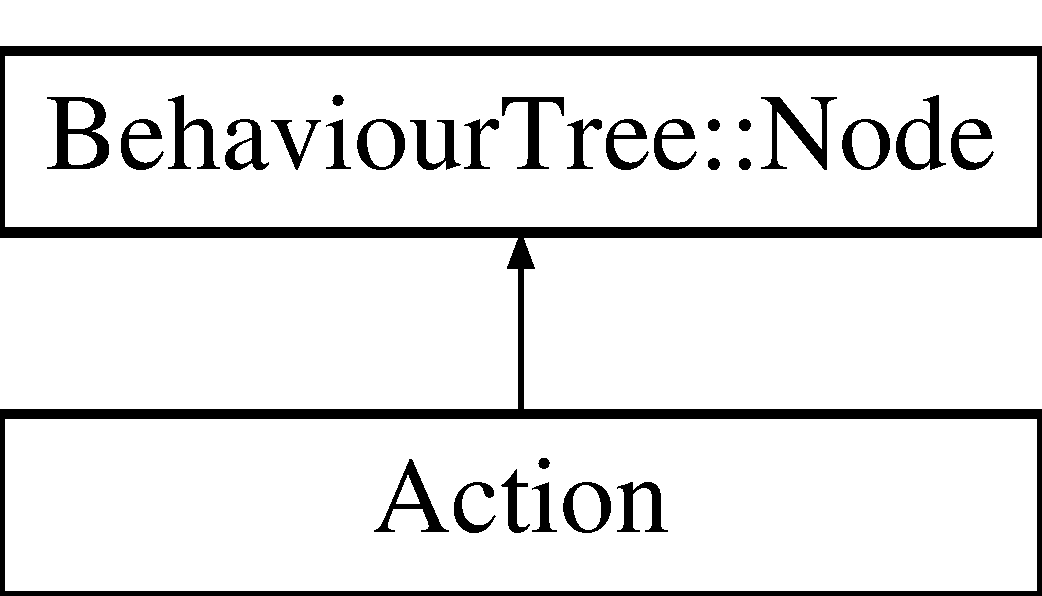
\includegraphics[height=2.000000cm]{class_action}
\end{center}
\end{figure}
\subsection*{Public Member Functions}
\begin{DoxyCompactItemize}
\item 
\mbox{\Hypertarget{class_action_adcc22e4c3499615de29737c0cb5544b9}\label{class_action_adcc22e4c3499615de29737c0cb5544b9}} 
{\bfseries Action} (\hyperlink{class_behaviour_tree}{Behaviour\+Tree} \&newbt, std\+::string new\+Name, bool isthere\+Item)
\end{DoxyCompactItemize}


The documentation for this class was generated from the following file\+:\begin{DoxyCompactItemize}
\item 
C\+:/\+Users/\+Alastair/\+Documents/\+Git\+Hub/comp250-\/\+A\+I-\/portfolio/\+Space\+Game/\+S\+D\+L\+\_\+project/Behaviour\+Tree.\+h\end{DoxyCompactItemize}

\hypertarget{class_agent}{}\section{Agent Class Reference}
\label{class_agent}\index{Agent@{Agent}}
\subsection*{Public Types}
\begin{DoxyCompactItemize}
\item 
enum \hyperlink{class_agent_af0b2c4596f7df623b5912509a09d0449}{agent\+Movement\+Status} \{ {\bfseries Idle}, 
{\bfseries Traversing\+Path}, 
{\bfseries Waiting}
 \}\begin{DoxyCompactList}\small\item\em Contains what the current status of the agent is doing. \end{DoxyCompactList}
\item 
enum \hyperlink{class_agent_ac7c6344403211868f101f7903fa9cb82}{agent\+Services\+Status} \{ \newline
{\bfseries NA}, 
{\bfseries Hungry}, 
{\bfseries Tired}, 
{\bfseries WC}, 
\newline
{\bfseries Suffocating}
 \}\begin{DoxyCompactList}\small\item\em Contains what the agent needs to do the most. \end{DoxyCompactList}
\end{DoxyCompactItemize}
\subsection*{Public Member Functions}
\begin{DoxyCompactItemize}
\item 
\mbox{\Hypertarget{class_agent_aa273213a1d5fbd26b473b6ed7c99ddb8}\label{class_agent_aa273213a1d5fbd26b473b6ed7c99ddb8}} 
void \hyperlink{class_agent_aa273213a1d5fbd26b473b6ed7c99ddb8}{Update} (\hyperlink{class_level}{Level} \&level)
\begin{DoxyCompactList}\small\item\em Update method for \hyperlink{class_agent}{Agent}. \end{DoxyCompactList}\item 
\mbox{\Hypertarget{class_agent_ab42895cf783c51c67a8719b7bdab9794}\label{class_agent_ab42895cf783c51c67a8719b7bdab9794}} 
void \hyperlink{class_agent_ab42895cf783c51c67a8719b7bdab9794}{Move} (\hyperlink{class_level}{Level} \&level, \hyperlink{class_point}{Point} \&Start\+Point, \hyperlink{class_point}{Point} \&End\+Point)
\begin{DoxyCompactList}\small\item\em Movement method for \hyperlink{class_agent}{Agent}. \end{DoxyCompactList}\item 
\mbox{\Hypertarget{class_agent_a207c925e3183a06c4ee6ce06d3d10f25}\label{class_agent_a207c925e3183a06c4ee6ce06d3d10f25}} 
int \hyperlink{class_agent_a207c925e3183a06c4ee6ce06d3d10f25}{getX} ()
\begin{DoxyCompactList}\small\item\em Gets the characters X value. \end{DoxyCompactList}\item 
\mbox{\Hypertarget{class_agent_ae354a9492265ed3686565676bbe27bf9}\label{class_agent_ae354a9492265ed3686565676bbe27bf9}} 
int \hyperlink{class_agent_ae354a9492265ed3686565676bbe27bf9}{getY} ()
\begin{DoxyCompactList}\small\item\em Gets the characters Y value. \end{DoxyCompactList}\item 
\mbox{\Hypertarget{class_agent_af8ae93713803f18c352981c6c96ed89e}\label{class_agent_af8ae93713803f18c352981c6c96ed89e}} 
int \hyperlink{class_agent_af8ae93713803f18c352981c6c96ed89e}{get\+CellX} ()
\begin{DoxyCompactList}\small\item\em Gets the characters X value. \end{DoxyCompactList}\item 
\mbox{\Hypertarget{class_agent_a73da67739c721597ad206901766c618a}\label{class_agent_a73da67739c721597ad206901766c618a}} 
int \hyperlink{class_agent_a73da67739c721597ad206901766c618a}{get\+CellY} ()
\begin{DoxyCompactList}\small\item\em Gets the characters Y value. \end{DoxyCompactList}\item 
\mbox{\Hypertarget{class_agent_a3acead21f857626ca791c8b911b4cfa4}\label{class_agent_a3acead21f857626ca791c8b911b4cfa4}} 
int \hyperlink{class_agent_a3acead21f857626ca791c8b911b4cfa4}{get\+Size} ()
\begin{DoxyCompactList}\small\item\em Gets the characters size. \end{DoxyCompactList}\item 
\mbox{\Hypertarget{class_agent_a8a5364ce3ed78c09ab47e91a02776e92}\label{class_agent_a8a5364ce3ed78c09ab47e91a02776e92}} 
double \hyperlink{class_agent_a8a5364ce3ed78c09ab47e91a02776e92}{get\+Speed} ()
\begin{DoxyCompactList}\small\item\em Gets the characters speed. \end{DoxyCompactList}\item 
\mbox{\Hypertarget{class_agent_a93cb897625e7650683cfb345e5d77559}\label{class_agent_a93cb897625e7650683cfb345e5d77559}} 
int \hyperlink{class_agent_a93cb897625e7650683cfb345e5d77559}{setX} (int newX)
\begin{DoxyCompactList}\small\item\em Sets the characters X value. \end{DoxyCompactList}\item 
\mbox{\Hypertarget{class_agent_a8105325d19923df18912578b28f702b1}\label{class_agent_a8105325d19923df18912578b28f702b1}} 
int \hyperlink{class_agent_a8105325d19923df18912578b28f702b1}{setY} (int newY)
\begin{DoxyCompactList}\small\item\em Sets the characters Y value. \end{DoxyCompactList}\item 
\mbox{\Hypertarget{class_agent_a579b5b77437e523552005066b12b9983}\label{class_agent_a579b5b77437e523552005066b12b9983}} 
int \hyperlink{class_agent_a579b5b77437e523552005066b12b9983}{set\+CellX} (int new\+CellX)
\begin{DoxyCompactList}\small\item\em Sets the characters cellX value. \end{DoxyCompactList}\item 
\mbox{\Hypertarget{class_agent_aa5e72b9928f0c0cfc7dd93240dbf6bfc}\label{class_agent_aa5e72b9928f0c0cfc7dd93240dbf6bfc}} 
int \hyperlink{class_agent_aa5e72b9928f0c0cfc7dd93240dbf6bfc}{set\+CellY} (int new\+CellY)
\begin{DoxyCompactList}\small\item\em Sets the characters cellY value. \end{DoxyCompactList}\item 
\mbox{\Hypertarget{class_agent_ad0b44c550842be01f5cf530eaaa1d21f}\label{class_agent_ad0b44c550842be01f5cf530eaaa1d21f}} 
int \hyperlink{class_agent_ad0b44c550842be01f5cf530eaaa1d21f}{set\+Position} (int newX, int newY)
\begin{DoxyCompactList}\small\item\em Sets the position that takes 2 arguments, x and y. \end{DoxyCompactList}\item 
\mbox{\Hypertarget{class_agent_a75e2e56c3a0a8bdee42ddc5750a06684}\label{class_agent_a75e2e56c3a0a8bdee42ddc5750a06684}} 
double \hyperlink{class_agent_a75e2e56c3a0a8bdee42ddc5750a06684}{set\+Speed} (double new\+Speed)
\begin{DoxyCompactList}\small\item\em Sets the characters current speed. \end{DoxyCompactList}\item 
\mbox{\Hypertarget{class_agent_a78215921c404b25326daa1ba3bf6d15d}\label{class_agent_a78215921c404b25326daa1ba3bf6d15d}} 
\hyperlink{class_point}{Point} \hyperlink{class_agent_a78215921c404b25326daa1ba3bf6d15d}{get\+Agent\+Point\+Location} ()
\begin{DoxyCompactList}\small\item\em Gets and sets the agents point location. \end{DoxyCompactList}\item 
\mbox{\Hypertarget{class_agent_a384d639479f5c149275780f4e39c64c7}\label{class_agent_a384d639479f5c149275780f4e39c64c7}} 
\hyperlink{class_point}{Point} {\bfseries set\+Agent\+Point\+Location} (\hyperlink{class_point}{Point} new\+Point\+Location)
\item 
\mbox{\Hypertarget{class_agent_af30ae01f87dcf622ceb50921ecaa3075}\label{class_agent_af30ae01f87dcf622ceb50921ecaa3075}} 
double \hyperlink{class_agent_af30ae01f87dcf622ceb50921ecaa3075}{get\+Health} ()
\begin{DoxyCompactList}\small\item\em Gets and Sets the agents health. \end{DoxyCompactList}\item 
\mbox{\Hypertarget{class_agent_abf38df47b1f8c4a183c655d80275cb20}\label{class_agent_abf38df47b1f8c4a183c655d80275cb20}} 
double {\bfseries set\+Health} (double new\+Health)
\item 
\mbox{\Hypertarget{class_agent_a51b835d48e31e09698ecdceb721c3f23}\label{class_agent_a51b835d48e31e09698ecdceb721c3f23}} 
double \hyperlink{class_agent_a51b835d48e31e09698ecdceb721c3f23}{get\+Hunger} ()
\begin{DoxyCompactList}\small\item\em Gets and Sets the agents hunger. \end{DoxyCompactList}\item 
\mbox{\Hypertarget{class_agent_a7f972fff138634c1b455e63db413c702}\label{class_agent_a7f972fff138634c1b455e63db413c702}} 
double {\bfseries set\+Hunger} (double new\+Hunger)
\item 
\mbox{\Hypertarget{class_agent_a5519977f67de721081136fe11efcd8c7}\label{class_agent_a5519977f67de721081136fe11efcd8c7}} 
double \hyperlink{class_agent_a5519977f67de721081136fe11efcd8c7}{get\+Tiredness} ()
\begin{DoxyCompactList}\small\item\em Gets and Sets the agents tiredness (Tiredness increaes from 0) \end{DoxyCompactList}\item 
\mbox{\Hypertarget{class_agent_a4a8525ce42c08122282051efe077c791}\label{class_agent_a4a8525ce42c08122282051efe077c791}} 
double {\bfseries set\+Tiredness} (double new\+Tiredness)
\item 
\mbox{\Hypertarget{class_agent_aa6910d23593e6e7fbff838e60585e79c}\label{class_agent_aa6910d23593e6e7fbff838e60585e79c}} 
double \hyperlink{class_agent_aa6910d23593e6e7fbff838e60585e79c}{get\+Toiet\+Need} ()
\begin{DoxyCompactList}\small\item\em Gets and Sets the agents tiredness (Tiredness increaes from 0) \end{DoxyCompactList}\item 
\mbox{\Hypertarget{class_agent_a0db1170e6cc50f37981a5ab305a181e0}\label{class_agent_a0db1170e6cc50f37981a5ab305a181e0}} 
double {\bfseries set\+Toilet\+Need} (double new\+Toilet\+Need)
\item 
\mbox{\Hypertarget{class_agent_a9abbdf8d3a9e2116faddce591865164b}\label{class_agent_a9abbdf8d3a9e2116faddce591865164b}} 
double \hyperlink{class_agent_a9abbdf8d3a9e2116faddce591865164b}{get\+Oxygen\+Level} ()
\begin{DoxyCompactList}\small\item\em Gets and Sets the agents oxygen level. \end{DoxyCompactList}\item 
\mbox{\Hypertarget{class_agent_a58c4462e557ee00c45b3a8a8186980ee}\label{class_agent_a58c4462e557ee00c45b3a8a8186980ee}} 
double {\bfseries set\+Oxygen\+Level} (double new\+Oxygen\+Level)
\end{DoxyCompactItemize}
\subsection*{Public Attributes}
\begin{DoxyCompactItemize}
\item 
\mbox{\Hypertarget{class_agent_a88eff9b9a41c730d03e1b14dd730fe72}\label{class_agent_a88eff9b9a41c730d03e1b14dd730fe72}} 
std\+::string \hyperlink{class_agent_a88eff9b9a41c730d03e1b14dd730fe72}{character\+Type} = \char`\"{}N\+PC\char`\"{}
\begin{DoxyCompactList}\small\item\em Character Type. \end{DoxyCompactList}\item 
\mbox{\Hypertarget{class_agent_ae4e1c9d4a042a0aa761392c45bed3a2b}\label{class_agent_ae4e1c9d4a042a0aa761392c45bed3a2b}} 
$\ast$Create an instance of pathfinder $\ast$\hyperlink{class_pathfinder}{Pathfinder} {\bfseries pathfinder}
\item 
\mbox{\Hypertarget{class_agent_ad221d98ce80b1f5ddd06182a825e50c5}\label{class_agent_ad221d98ce80b1f5ddd06182a825e50c5}} 
std\+::vector$<$ \hyperlink{class_point}{Point} $>$ \hyperlink{class_agent_ad221d98ce80b1f5ddd06182a825e50c5}{path}
\begin{DoxyCompactList}\small\item\em Conains the list of nodes that makes the path. \end{DoxyCompactList}\item 
\mbox{\Hypertarget{class_agent_a2d0b3cc1362a8bbbddda3476573f6733}\label{class_agent_a2d0b3cc1362a8bbbddda3476573f6733}} 
\hyperlink{class_agent_af0b2c4596f7df623b5912509a09d0449}{agent\+Movement\+Status} {\bfseries movement\+Status} = Idle
\item 
\mbox{\Hypertarget{class_agent_a38888c7ca94b440873b5ea3b2c01e52f}\label{class_agent_a38888c7ca94b440873b5ea3b2c01e52f}} 
\hyperlink{class_agent_ac7c6344403211868f101f7903fa9cb82}{agent\+Services\+Status} {\bfseries agent\+Need} = NA
\item 
\mbox{\Hypertarget{class_agent_aab5675be1775cd18ff37e3e1870d51be}\label{class_agent_aab5675be1775cd18ff37e3e1870d51be}} 
bool {\bfseries is\+Moving} = false
\item 
\mbox{\Hypertarget{class_agent_ac256f4583cc7f7c581ee1f7250f05f4f}\label{class_agent_ac256f4583cc7f7c581ee1f7250f05f4f}} 
bool \hyperlink{class_agent_ac256f4583cc7f7c581ee1f7250f05f4f}{is\+Alive} = true
\begin{DoxyCompactList}\small\item\em Boolean for whether character is alive. \end{DoxyCompactList}\item 
\mbox{\Hypertarget{class_agent_af3384cfb4c86b2ca093ad02a4ce57d37}\label{class_agent_af3384cfb4c86b2ca093ad02a4ce57d37}} 
bool {\bfseries agent\+Wonder\+When\+Idle} = false
\item 
\mbox{\Hypertarget{class_agent_ab150cbcd976d2c50b1f34503c3a98168}\label{class_agent_ab150cbcd976d2c50b1f34503c3a98168}} 
bool {\bfseries agent\+Can\+Rotate} = true
\item 
\mbox{\Hypertarget{class_agent_a02a2a7245b8677b8bcdf3bd311f5a420}\label{class_agent_a02a2a7245b8677b8bcdf3bd311f5a420}} 
int {\bfseries agent\+Rotation} = 0
\end{DoxyCompactItemize}


\subsection{Member Enumeration Documentation}
\mbox{\Hypertarget{class_agent_af0b2c4596f7df623b5912509a09d0449}\label{class_agent_af0b2c4596f7df623b5912509a09d0449}} 
\index{Agent@{Agent}!agent\+Movement\+Status@{agent\+Movement\+Status}}
\index{agent\+Movement\+Status@{agent\+Movement\+Status}!Agent@{Agent}}
\subsubsection{\texorpdfstring{agent\+Movement\+Status}{agentMovementStatus}}
{\footnotesize\ttfamily enum \hyperlink{class_agent_af0b2c4596f7df623b5912509a09d0449}{Agent\+::agent\+Movement\+Status}}



Contains what the current status of the agent is doing. 

Types of agent state\+: (Idle, Found\+Path, Dead...) \mbox{\Hypertarget{class_agent_ac7c6344403211868f101f7903fa9cb82}\label{class_agent_ac7c6344403211868f101f7903fa9cb82}} 
\index{Agent@{Agent}!agent\+Services\+Status@{agent\+Services\+Status}}
\index{agent\+Services\+Status@{agent\+Services\+Status}!Agent@{Agent}}
\subsubsection{\texorpdfstring{agent\+Services\+Status}{agentServicesStatus}}
{\footnotesize\ttfamily enum \hyperlink{class_agent_ac7c6344403211868f101f7903fa9cb82}{Agent\+::agent\+Services\+Status}}



Contains what the agent needs to do the most. 

Types of agent state\+: (Food, WC, Bed...) 

The documentation for this class was generated from the following files\+:\begin{DoxyCompactItemize}
\item 
C\+:/\+Users/\+Alastair/\+Documents/\+Git\+Hub/comp250-\/\+A\+I-\/portfolio/\+Space\+Game/\+S\+D\+L\+\_\+project/Agent.\+h\item 
C\+:/\+Users/\+Alastair/\+Documents/\+Git\+Hub/comp250-\/\+A\+I-\/portfolio/\+Space\+Game/\+S\+D\+L\+\_\+project/Agent.\+cpp\end{DoxyCompactItemize}

\hypertarget{class_agent_behaviour}{}\section{Agent\+Behaviour Class Reference}
\label{class_agent_behaviour}\index{Agent\+Behaviour@{Agent\+Behaviour}}
\subsection*{Public Member Functions}
\begin{DoxyCompactItemize}
\item 
\mbox{\Hypertarget{class_agent_behaviour_afbb7103a8960b8b1982b71d25c036e71}\label{class_agent_behaviour_afbb7103a8960b8b1982b71d25c036e71}} 
\hyperlink{class_point}{Point} \hyperlink{class_agent_behaviour_afbb7103a8960b8b1982b71d25c036e71}{Find\+Nearest\+Cellto\+Agent} (\hyperlink{class_agent}{Agent} \&agent, \hyperlink{class_level}{Level} \&level, std\+::string cell\+Type)
\begin{DoxyCompactList}\small\item\em Finds the nearest cell to the agent from the string cell\+Type (e.\+g. \char`\"{}\+B\+E\+D\char`\"{} $\vert$$\vert$ \char`\"{}\+T\+O\+I\+L\+E\+T\char`\"{}) \end{DoxyCompactList}\item 
\mbox{\Hypertarget{class_agent_behaviour_a2a4f982b17f2bc0c7753aff6441d2667}\label{class_agent_behaviour_a2a4f982b17f2bc0c7753aff6441d2667}} 
void \hyperlink{class_agent_behaviour_a2a4f982b17f2bc0c7753aff6441d2667}{Decide\+Task} (\hyperlink{class_level}{Level} \&level, \hyperlink{class_agent}{Agent} \&agent)
\begin{DoxyCompactList}\small\item\em To Decide what task needs to be done. \end{DoxyCompactList}\item 
\mbox{\Hypertarget{class_agent_behaviour_a8f86aedeaebdab4553e0fe04e8593999}\label{class_agent_behaviour_a8f86aedeaebdab4553e0fe04e8593999}} 
void \hyperlink{class_agent_behaviour_a8f86aedeaebdab4553e0fe04e8593999}{Update\+Level\+Info} (\hyperlink{class_level}{Level} \&level, int cellX, int cellY)
\begin{DoxyCompactList}\small\item\em Updates some of the local class varaibles that store info about the level and what it contains for ease of use by behaviour tree. \end{DoxyCompactList}\end{DoxyCompactItemize}
\subsection*{Public Attributes}
\begin{DoxyCompactItemize}
\item 
\mbox{\Hypertarget{class_agent_behaviour_a2b26dafd1b01890c52803f19b18f846a}\label{class_agent_behaviour_a2b26dafd1b01890c52803f19b18f846a}} 
bool \hyperlink{class_agent_behaviour_a2b26dafd1b01890c52803f19b18f846a}{level\+Has\+Bed} = false
\begin{DoxyCompactList}\small\item\em Bool that stores whether the level has a bed. \end{DoxyCompactList}\item 
\mbox{\Hypertarget{class_agent_behaviour_a30450ea561add5573dffeb78b32e3bca}\label{class_agent_behaviour_a30450ea561add5573dffeb78b32e3bca}} 
std\+::vector$<$ \hyperlink{class_point}{Point} $>$ \hyperlink{class_agent_behaviour_a30450ea561add5573dffeb78b32e3bca}{empty\+Bed\+Locations}
\begin{DoxyCompactList}\small\item\em A vector that stores empty bed locations. \end{DoxyCompactList}\item 
\mbox{\Hypertarget{class_agent_behaviour_af3def48bbce26581630f0f1cf3d2f67e}\label{class_agent_behaviour_af3def48bbce26581630f0f1cf3d2f67e}} 
bool \hyperlink{class_agent_behaviour_af3def48bbce26581630f0f1cf3d2f67e}{Level\+Has\+Toilet} = false
\begin{DoxyCompactList}\small\item\em Bool that stores whether the level has a toilet. \end{DoxyCompactList}\item 
\mbox{\Hypertarget{class_agent_behaviour_ad2018440fabd1aaad74f6ce3c22c64f1}\label{class_agent_behaviour_ad2018440fabd1aaad74f6ce3c22c64f1}} 
std\+::vector$<$ \hyperlink{class_point}{Point} $>$ \hyperlink{class_agent_behaviour_ad2018440fabd1aaad74f6ce3c22c64f1}{empty\+Toilet\+Locations}
\begin{DoxyCompactList}\small\item\em A vector that stores empty toilet locations. \end{DoxyCompactList}\item 
\mbox{\Hypertarget{class_agent_behaviour_ac541d443fc80b6c5d7758533d554648f}\label{class_agent_behaviour_ac541d443fc80b6c5d7758533d554648f}} 
int {\bfseries local\+Search\+Size} = 2
\end{DoxyCompactItemize}


The documentation for this class was generated from the following files\+:\begin{DoxyCompactItemize}
\item 
C\+:/\+Users/\+Alastair/\+Documents/\+Git\+Hub/comp250-\/\+A\+I-\/portfolio/\+Space\+Game/\+S\+D\+L\+\_\+project/Agent\+Behaviour.\+h\item 
C\+:/\+Users/\+Alastair/\+Documents/\+Git\+Hub/comp250-\/\+A\+I-\/portfolio/\+Space\+Game/\+S\+D\+L\+\_\+project/Agent\+Behaviour.\+cpp\end{DoxyCompactItemize}

\hypertarget{class_agent_manager}{}\section{Agent\+Manager Class Reference}
\label{class_agent_manager}\index{Agent\+Manager@{Agent\+Manager}}


The abstract character class.  




{\ttfamily \#include $<$Agent\+Manager.\+h$>$}

\subsection*{Public Member Functions}
\begin{DoxyCompactItemize}
\item 
\mbox{\Hypertarget{class_agent_manager_a49ff5a8f60bae1c0b8d6c9aeda8f6961}\label{class_agent_manager_a49ff5a8f60bae1c0b8d6c9aeda8f6961}} 
\hyperlink{class_agent_manager_a49ff5a8f60bae1c0b8d6c9aeda8f6961}{Agent\+Manager} ()
\begin{DoxyCompactList}\small\item\em A constructor. \end{DoxyCompactList}\item 
\mbox{\Hypertarget{class_agent_manager_a6b3efb95b74c9c96b9dbaf0868f17759}\label{class_agent_manager_a6b3efb95b74c9c96b9dbaf0868f17759}} 
\hyperlink{class_agent_manager_a6b3efb95b74c9c96b9dbaf0868f17759}{$\sim$\+Agent\+Manager} ()
\begin{DoxyCompactList}\small\item\em A destructor. \end{DoxyCompactList}\item 
\mbox{\Hypertarget{class_agent_manager_aeb29779b8f17a2a4b0583ba45ec88e21}\label{class_agent_manager_aeb29779b8f17a2a4b0583ba45ec88e21}} 
void {\bfseries Update\+Agents} (std\+::vector$<$ \hyperlink{class_agent}{Agent} $>$ \&\hyperlink{class_agent_manager_a599aa8ac7b9ac078c77b493278d2b6da}{all\+Agents}, S\+D\+L\+\_\+\+Renderer $\ast$renderer, \hyperlink{class_level}{Level} \&level)
\item 
\mbox{\Hypertarget{class_agent_manager_a23fa29fff7f4ce6e01b4c4cd1757be6a}\label{class_agent_manager_a23fa29fff7f4ce6e01b4c4cd1757be6a}} 
void {\bfseries Render\+Agents} (\hyperlink{class_agent}{Agent} \&agent, S\+D\+L\+\_\+\+Renderer $\ast$renderer, \hyperlink{class_level}{Level} \&level)
\item 
\mbox{\Hypertarget{class_agent_manager_a67b4e05ac1f86c7cb3cf5d5ea0573b91}\label{class_agent_manager_a67b4e05ac1f86c7cb3cf5d5ea0573b91}} 
void \hyperlink{class_agent_manager_a67b4e05ac1f86c7cb3cf5d5ea0573b91}{Spawn\+Agent} (std\+::string Character\+Type\+Var, std\+::vector$<$ \hyperlink{class_agent}{Agent} $>$ \&\hyperlink{class_agent_manager_a599aa8ac7b9ac078c77b493278d2b6da}{all\+Agents}, int x, int y)
\begin{DoxyCompactList}\small\item\em Spawn character function (Character types are (N\+PC, Player) \end{DoxyCompactList}\item 
\mbox{\Hypertarget{class_agent_manager_ab99bb1f844d39a407c73ab8ec57c8a8a}\label{class_agent_manager_ab99bb1f844d39a407c73ab8ec57c8a8a}} 
void \hyperlink{class_agent_manager_ab99bb1f844d39a407c73ab8ec57c8a8a}{Erase\+All\+Agent\+Paths} (std\+::vector$<$ \hyperlink{class_agent}{Agent} $>$ \&\hyperlink{class_agent_manager_a599aa8ac7b9ac078c77b493278d2b6da}{all\+Agents})
\begin{DoxyCompactList}\small\item\em Erases all the agents path. \end{DoxyCompactList}\item 
\mbox{\Hypertarget{class_agent_manager_aeb752dda5f920cadcf18f5e5ee90b2d6}\label{class_agent_manager_aeb752dda5f920cadcf18f5e5ee90b2d6}} 
void \hyperlink{class_agent_manager_aeb752dda5f920cadcf18f5e5ee90b2d6}{Erase\+All\+Agents} (std\+::vector$<$ \hyperlink{class_agent}{Agent} $>$ \&\hyperlink{class_agent_manager_a599aa8ac7b9ac078c77b493278d2b6da}{all\+Agents})
\begin{DoxyCompactList}\small\item\em Erases all the agents in the game. \end{DoxyCompactList}\end{DoxyCompactItemize}
\subsection*{Public Attributes}
\begin{DoxyCompactItemize}
\item 
\mbox{\Hypertarget{class_agent_manager_ac83790e3aa445b1c1547d4c9a9016cb2}\label{class_agent_manager_ac83790e3aa445b1c1547d4c9a9016cb2}} 
\hyperlink{class_agent_behaviour}{Agent\+Behaviour} \hyperlink{class_agent_manager_ac83790e3aa445b1c1547d4c9a9016cb2}{agent\+Behaviour}
\begin{DoxyCompactList}\small\item\em Create an instance of Agent\+Behavour. \end{DoxyCompactList}\item 
\mbox{\Hypertarget{class_agent_manager_a599aa8ac7b9ac078c77b493278d2b6da}\label{class_agent_manager_a599aa8ac7b9ac078c77b493278d2b6da}} 
std\+::vector$<$ \hyperlink{class_agent}{Agent} $>$ \hyperlink{class_agent_manager_a599aa8ac7b9ac078c77b493278d2b6da}{all\+Agents}
\begin{DoxyCompactList}\small\item\em Contains a list of all the characters. \end{DoxyCompactList}\item 
\mbox{\Hypertarget{class_agent_manager_a7d43712823386d03a70dede42b1358e2}\label{class_agent_manager_a7d43712823386d03a70dede42b1358e2}} 
bool \hyperlink{class_agent_manager_a7d43712823386d03a70dede42b1358e2}{render\+Stats} = true
\begin{DoxyCompactList}\small\item\em Whether the game will render agent stats. \end{DoxyCompactList}\item 
\mbox{\Hypertarget{class_agent_manager_a6b8f87746c5ff0deef91b13e5d1983c6}\label{class_agent_manager_a6b8f87746c5ff0deef91b13e5d1983c6}} 
bool \hyperlink{class_agent_manager_a6b8f87746c5ff0deef91b13e5d1983c6}{draw\+Agent\+Paths} = true
\begin{DoxyCompactList}\small\item\em Whether the game will draw the agent paths. \end{DoxyCompactList}\end{DoxyCompactItemize}


\subsection{Detailed Description}
The abstract character class. 

This class is the controller for the \hyperlink{class_agent}{Agent} class and will manage how the agents behave. 

The documentation for this class was generated from the following files\+:\begin{DoxyCompactItemize}
\item 
C\+:/\+Users/\+Alastair/\+Documents/\+Git\+Hub/comp250-\/\+A\+I-\/portfolio/\+Space\+Game/\+S\+D\+L\+\_\+project/Agent\+Manager.\+h\item 
C\+:/\+Users/\+Alastair/\+Documents/\+Git\+Hub/comp250-\/\+A\+I-\/portfolio/\+Space\+Game/\+S\+D\+L\+\_\+project/Agent\+Manager.\+cpp\end{DoxyCompactItemize}

\hypertarget{class_behaviour_tree}{}\section{Behaviour\+Tree Class Reference}
\label{class_behaviour_tree}\index{Behaviour\+Tree@{Behaviour\+Tree}}
\subsection*{Classes}
\begin{DoxyCompactItemize}
\item 
class \hyperlink{class_behaviour_tree_1_1_composite_node}{Composite\+Node}
\item 
class \hyperlink{class_behaviour_tree_1_1_node}{Node}
\item 
class \hyperlink{class_behaviour_tree_1_1_root}{Root}
\item 
class \hyperlink{class_behaviour_tree_1_1_selector}{Selector}
\item 
class \hyperlink{class_behaviour_tree_1_1_sequence}{Sequence}
\end{DoxyCompactItemize}
\subsection*{Public Member Functions}
\begin{DoxyCompactItemize}
\item 
\mbox{\Hypertarget{class_behaviour_tree_a0cc081b0682612c13405f6ce5ed0f8a1}\label{class_behaviour_tree_a0cc081b0682612c13405f6ce5ed0f8a1}} 
void {\bfseries set\+Root\+Child} (\hyperlink{class_behaviour_tree_1_1_node}{Node} $\ast$root\+Child) const
\item 
\mbox{\Hypertarget{class_behaviour_tree_accac405f3dcd9c4138285abcc0ad4316}\label{class_behaviour_tree_accac405f3dcd9c4138285abcc0ad4316}} 
bool {\bfseries run} () const
\end{DoxyCompactItemize}
\subsection*{Public Attributes}
\begin{DoxyCompactItemize}
\item 
\mbox{\Hypertarget{class_behaviour_tree_a604c07c4745e49dc974d766b0898f9ad}\label{class_behaviour_tree_a604c07c4745e49dc974d766b0898f9ad}} 
std\+::string {\bfseries leaf\+Node\+To\+Run} = \char`\"{}NA\char`\"{}
\end{DoxyCompactItemize}


The documentation for this class was generated from the following file\+:\begin{DoxyCompactItemize}
\item 
C\+:/\+Users/\+Alastair/\+Documents/\+Git\+Hub/comp250-\/\+A\+I-\/portfolio/\+Space\+Game/\+S\+D\+L\+\_\+project/Behaviour\+Tree.\+h\end{DoxyCompactItemize}

\hypertarget{class_cargo_ship}{}\section{Cargo\+Ship Class Reference}
\label{class_cargo_ship}\index{Cargo\+Ship@{Cargo\+Ship}}
Inheritance diagram for Cargo\+Ship\+:\begin{figure}[H]
\begin{center}
\leavevmode
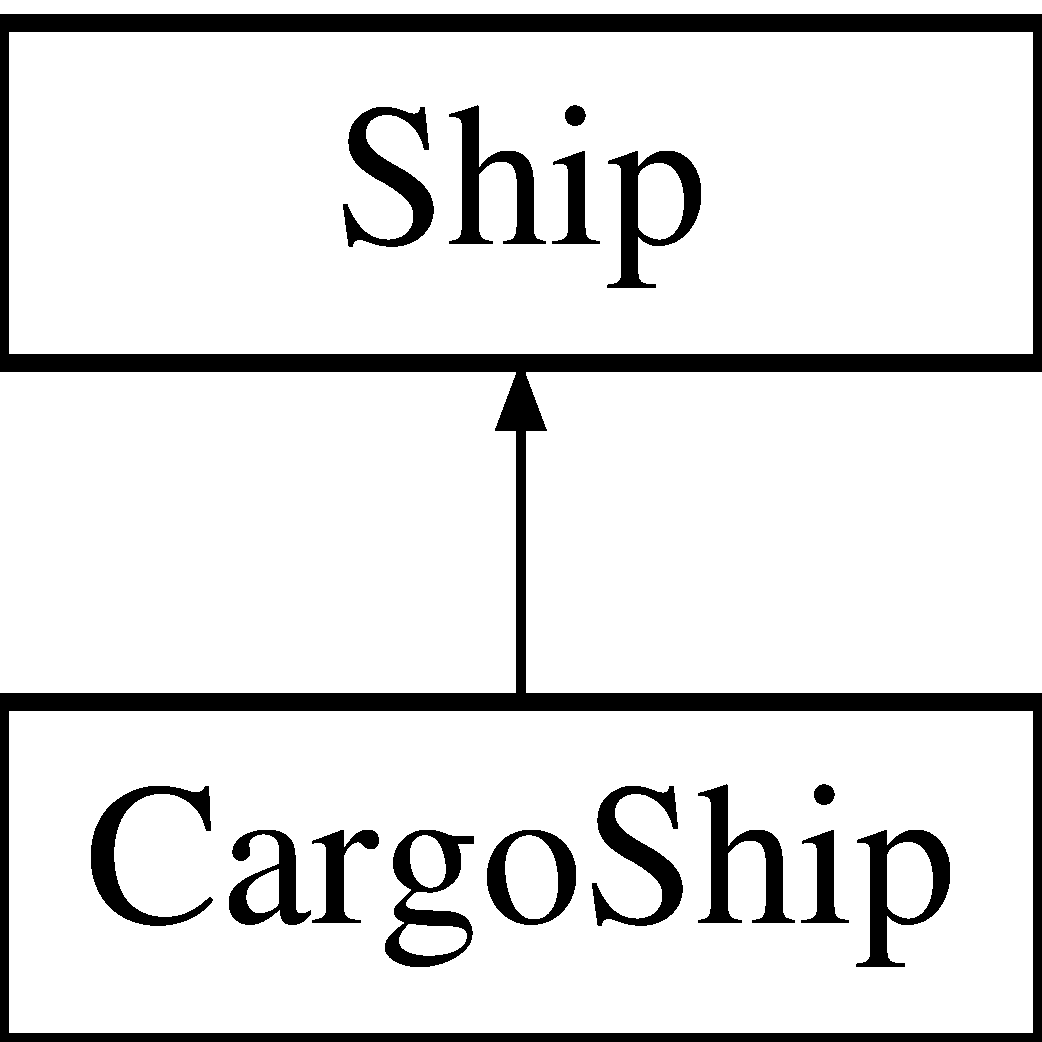
\includegraphics[height=2.000000cm]{class_cargo_ship}
\end{center}
\end{figure}
\subsection*{Public Member Functions}
\begin{DoxyCompactItemize}
\item 
\mbox{\Hypertarget{class_cargo_ship_a8cb7bc3c5f733c1d9972c348f65de1d8}\label{class_cargo_ship_a8cb7bc3c5f733c1d9972c348f65de1d8}} 
\hyperlink{class_cargo_ship_a8cb7bc3c5f733c1d9972c348f65de1d8}{Cargo\+Ship} ()
\begin{DoxyCompactList}\small\item\em Constructor. \end{DoxyCompactList}\item 
\mbox{\Hypertarget{class_cargo_ship_ab1574d0f229f183091a822b9b2e857c5}\label{class_cargo_ship_ab1574d0f229f183091a822b9b2e857c5}} 
\hyperlink{class_cargo_ship_ab1574d0f229f183091a822b9b2e857c5}{$\sim$\+Cargo\+Ship} ()
\begin{DoxyCompactList}\small\item\em Destructor. \end{DoxyCompactList}\end{DoxyCompactItemize}
\subsection*{Additional Inherited Members}


The documentation for this class was generated from the following files\+:\begin{DoxyCompactItemize}
\item 
C\+:/\+Users/\+Alastair/\+Documents/\+Git\+Hub/comp250-\/\+A\+I-\/portfolio/\+Space\+Game/\+S\+D\+L\+\_\+project/Cargo\+Ship.\+h\item 
C\+:/\+Users/\+Alastair/\+Documents/\+Git\+Hub/comp250-\/\+A\+I-\/portfolio/\+Space\+Game/\+S\+D\+L\+\_\+project/Cargo\+Ship.\+cpp\end{DoxyCompactItemize}

\hypertarget{class_cell}{}\section{Cell Class Reference}
\label{class_cell}\index{Cell@{Cell}}
\subsection*{Public Member Functions}
\begin{DoxyCompactItemize}
\item 
\mbox{\Hypertarget{class_cell_a394510643e8664cf12b5efaf5cb99f71}\label{class_cell_a394510643e8664cf12b5efaf5cb99f71}} 
\hyperlink{class_cell_a394510643e8664cf12b5efaf5cb99f71}{Cell} ()
\begin{DoxyCompactList}\small\item\em A constructor. \end{DoxyCompactList}\item 
\hyperlink{class_cell_aa39ad04eeebb7bf00d592ad36640337e}{Cell} (int x, int y)
\begin{DoxyCompactList}\small\item\em An alternate constructor. \end{DoxyCompactList}\item 
\mbox{\Hypertarget{class_cell_a9fa559f7a28e2b4336c6879ca09304d8}\label{class_cell_a9fa559f7a28e2b4336c6879ca09304d8}} 
\hyperlink{class_cell_a9fa559f7a28e2b4336c6879ca09304d8}{$\sim$\+Cell} ()
\begin{DoxyCompactList}\small\item\em A destructor. \end{DoxyCompactList}\item 
\mbox{\Hypertarget{class_cell_a40caf41e5ab28c67e0e8c547eb5281ee}\label{class_cell_a40caf41e5ab28c67e0e8c547eb5281ee}} 
int \hyperlink{class_cell_a40caf41e5ab28c67e0e8c547eb5281ee}{getX} () const
\begin{DoxyCompactList}\small\item\em Gets the \hyperlink{class_cell}{Cell}\textquotesingle{}s X value. \end{DoxyCompactList}\item 
\mbox{\Hypertarget{class_cell_a0dc1e0edf77cb2c49840928025ef7360}\label{class_cell_a0dc1e0edf77cb2c49840928025ef7360}} 
int \hyperlink{class_cell_a0dc1e0edf77cb2c49840928025ef7360}{getY} () const
\begin{DoxyCompactList}\small\item\em Gets the \hyperlink{class_cell}{Cell}\textquotesingle{}s Y value. \end{DoxyCompactList}\item 
\mbox{\Hypertarget{class_cell_a2f33cee2863b092b4bf0bca50d6a0e58}\label{class_cell_a2f33cee2863b092b4bf0bca50d6a0e58}} 
int \hyperlink{class_cell_a2f33cee2863b092b4bf0bca50d6a0e58}{get\+Oxygen\+Level} ()
\begin{DoxyCompactList}\small\item\em Gets the \hyperlink{class_cell}{Cell}\textquotesingle{}s oxygen\+Level. \end{DoxyCompactList}\item 
\mbox{\Hypertarget{class_cell_a989cee545edaa818bab0ae6627419250}\label{class_cell_a989cee545edaa818bab0ae6627419250}} 
int \hyperlink{class_cell_a989cee545edaa818bab0ae6627419250}{setX} (int newX)
\begin{DoxyCompactList}\small\item\em Sets the Cells X value. \end{DoxyCompactList}\item 
\mbox{\Hypertarget{class_cell_a4cc90d99e603947aca4d36636c5868f8}\label{class_cell_a4cc90d99e603947aca4d36636c5868f8}} 
int \hyperlink{class_cell_a4cc90d99e603947aca4d36636c5868f8}{setY} (int newY)
\begin{DoxyCompactList}\small\item\em Sets the Cells Y value. \end{DoxyCompactList}\item 
\mbox{\Hypertarget{class_cell_a15a5726bfb5e111fb3de449a70107b36}\label{class_cell_a15a5726bfb5e111fb3de449a70107b36}} 
int \hyperlink{class_cell_a15a5726bfb5e111fb3de449a70107b36}{set\+Oxygen\+Level} (int new\+Oxygen\+Level)
\begin{DoxyCompactList}\small\item\em Sets the \hyperlink{class_cell}{Cell}\textquotesingle{}s oxygen\+Level. \end{DoxyCompactList}\end{DoxyCompactItemize}
\subsection*{Public Attributes}
\begin{DoxyCompactItemize}
\item 
\mbox{\Hypertarget{class_cell_ae044a0c1ef1dd0ca08ffe22c4b763433}\label{class_cell_ae044a0c1ef1dd0ca08ffe22c4b763433}} 
bool \hyperlink{class_cell_ae044a0c1ef1dd0ca08ffe22c4b763433}{is\+Room} = false
\begin{DoxyCompactList}\small\item\em Whether the cell is part of a room. \end{DoxyCompactList}\item 
\mbox{\Hypertarget{class_cell_a69d99aeda5f9117695c42ed209b7cf60}\label{class_cell_a69d99aeda5f9117695c42ed209b7cf60}} 
bool \hyperlink{class_cell_a69d99aeda5f9117695c42ed209b7cf60}{is\+Walkable} = false
\begin{DoxyCompactList}\small\item\em Whether the cell is walkable. \end{DoxyCompactList}\item 
\mbox{\Hypertarget{class_cell_a6d40064791a7160a9bb85a2e47a8dff4}\label{class_cell_a6d40064791a7160a9bb85a2e47a8dff4}} 
bool \hyperlink{class_cell_a6d40064791a7160a9bb85a2e47a8dff4}{is\+Open\+Door} = false
\begin{DoxyCompactList}\small\item\em Whether the cell is a door is open. \end{DoxyCompactList}\item 
\mbox{\Hypertarget{class_cell_aedef9250bc88ff0c02b6fd43be0d3a64}\label{class_cell_aedef9250bc88ff0c02b6fd43be0d3a64}} 
bool \hyperlink{class_cell_aedef9250bc88ff0c02b6fd43be0d3a64}{is\+Closed\+Door} = false
\begin{DoxyCompactList}\small\item\em Whether the cell door is closed. \end{DoxyCompactList}\item 
\mbox{\Hypertarget{class_cell_add0d783175466a8c4122d51262496306}\label{class_cell_add0d783175466a8c4122d51262496306}} 
bool \hyperlink{class_cell_add0d783175466a8c4122d51262496306}{is\+Goal} = false
\begin{DoxyCompactList}\small\item\em Represents the goal for the player. \end{DoxyCompactList}\item 
\mbox{\Hypertarget{class_cell_aaa5ccf51c9cd5d1500af0f7481b5588e}\label{class_cell_aaa5ccf51c9cd5d1500af0f7481b5588e}} 
int \hyperlink{class_cell_aaa5ccf51c9cd5d1500af0f7481b5588e}{oxygen\+Level} = 100
\begin{DoxyCompactList}\small\item\em The oxygen\+Level of the cell. \end{DoxyCompactList}\item 
\mbox{\Hypertarget{class_cell_a6cc1b533215a2fe1a0ba96265b43997f}\label{class_cell_a6cc1b533215a2fe1a0ba96265b43997f}} 
bool \hyperlink{class_cell_a6cc1b533215a2fe1a0ba96265b43997f}{is\+On\+Fire} = false
\begin{DoxyCompactList}\small\item\em Whether the cell is on fire. \end{DoxyCompactList}\item 
\mbox{\Hypertarget{class_cell_a408414f3a38c859dec3df3a6bd05bb1f}\label{class_cell_a408414f3a38c859dec3df3a6bd05bb1f}} 
bool \hyperlink{class_cell_a408414f3a38c859dec3df3a6bd05bb1f}{is\+Hull\+Breach} = false
\begin{DoxyCompactList}\small\item\em Whether the cell is a hull breach. \end{DoxyCompactList}\item 
\mbox{\Hypertarget{class_cell_ab789483cf35f76b8f90b1460330f7f80}\label{class_cell_ab789483cf35f76b8f90b1460330f7f80}} 
bool \hyperlink{class_cell_ab789483cf35f76b8f90b1460330f7f80}{is\+Oxygen\+Tank} = false
\begin{DoxyCompactList}\small\item\em Whether the cell is an oxygen tank. \end{DoxyCompactList}\item 
\mbox{\Hypertarget{class_cell_a865f48549b919d63c44672d06eddc03a}\label{class_cell_a865f48549b919d63c44672d06eddc03a}} 
bool \hyperlink{class_cell_a865f48549b919d63c44672d06eddc03a}{is\+Health\+Pack} = false
\begin{DoxyCompactList}\small\item\em Whether the cell is an \hyperlink{class_fire}{Fire} extengusher. \end{DoxyCompactList}\item 
\mbox{\Hypertarget{class_cell_af7efe7d40df1cd80a589820bb2c1b388}\label{class_cell_af7efe7d40df1cd80a589820bb2c1b388}} 
bool \hyperlink{class_cell_af7efe7d40df1cd80a589820bb2c1b388}{is\+Docking\+Path} = false
\begin{DoxyCompactList}\small\item\em Whether the cell is the dockingpath. \end{DoxyCompactList}\item 
\mbox{\Hypertarget{class_cell_a0cc30157bc1bde69b8e5cbaab05038f5}\label{class_cell_a0cc30157bc1bde69b8e5cbaab05038f5}} 
bool \hyperlink{class_cell_a0cc30157bc1bde69b8e5cbaab05038f5}{is\+Ship\+Cargo\+Bay} = false
\begin{DoxyCompactList}\small\item\em Whether the cell is part of the ships cargo bay. \end{DoxyCompactList}\item 
\mbox{\Hypertarget{class_cell_a1b083abd6436982134aebcbce16d6241}\label{class_cell_a1b083abd6436982134aebcbce16d6241}} 
bool \hyperlink{class_cell_a1b083abd6436982134aebcbce16d6241}{is\+Vertical\+Airlock} = false
\begin{DoxyCompactList}\small\item\em Whether the cell is a vertical airlock. \end{DoxyCompactList}\item 
\mbox{\Hypertarget{class_cell_a9f3ad57a5595ca4fa50f088f8bbab832}\label{class_cell_a9f3ad57a5595ca4fa50f088f8bbab832}} 
bool \hyperlink{class_cell_a9f3ad57a5595ca4fa50f088f8bbab832}{is\+Airlock\+Wall} = false
\begin{DoxyCompactList}\small\item\em Whether the cell is a airlock side. \end{DoxyCompactList}\item 
\mbox{\Hypertarget{class_cell_af25186ff716665d0ca7fdc38a8672253}\label{class_cell_af25186ff716665d0ca7fdc38a8672253}} 
bool \hyperlink{class_cell_af25186ff716665d0ca7fdc38a8672253}{is\+Cargo} = false
\begin{DoxyCompactList}\small\item\em Whetehr the cell is cargo. \end{DoxyCompactList}\item 
\mbox{\Hypertarget{class_cell_a6b1c886b18165fa9eb8282ab50a514d6}\label{class_cell_a6b1c886b18165fa9eb8282ab50a514d6}} 
bool \hyperlink{class_cell_a6b1c886b18165fa9eb8282ab50a514d6}{is\+Hydroponics\+Bay} = false
\begin{DoxyCompactList}\small\item\em Whether the cell is a hydroponics bay. \end{DoxyCompactList}\item 
\mbox{\Hypertarget{class_cell_ac9ff663273f018a96d2ab9a727fc8a5c}\label{class_cell_ac9ff663273f018a96d2ab9a727fc8a5c}} 
std\+::string {\bfseries hydroponics\+Orientation} = \char`\"{}NA\char`\"{}
\item 
\mbox{\Hypertarget{class_cell_a90887fb2f575d1938926eb2d538a333b}\label{class_cell_a90887fb2f575d1938926eb2d538a333b}} 
bool \hyperlink{class_cell_a90887fb2f575d1938926eb2d538a333b}{is\+Bed} = false
\begin{DoxyCompactList}\small\item\em Whether the cell is a bed. \end{DoxyCompactList}\item 
\mbox{\Hypertarget{class_cell_ac653b32cbc54e679883ad9699557f86c}\label{class_cell_ac653b32cbc54e679883ad9699557f86c}} 
bool \hyperlink{class_cell_ac653b32cbc54e679883ad9699557f86c}{is\+Occupied\+Bed} = false
\begin{DoxyCompactList}\small\item\em Wehther the cell is a bed and in use. \end{DoxyCompactList}\item 
\mbox{\Hypertarget{class_cell_a850b57eb873da4733a5253ecf432fb29}\label{class_cell_a850b57eb873da4733a5253ecf432fb29}} 
bool \hyperlink{class_cell_a850b57eb873da4733a5253ecf432fb29}{is\+Toilet} = false
\begin{DoxyCompactList}\small\item\em Whether the cell is a toilet. \end{DoxyCompactList}\item 
\mbox{\Hypertarget{class_cell_a31692ab53e4de80fd78153acb4553bb3}\label{class_cell_a31692ab53e4de80fd78153acb4553bb3}} 
bool \hyperlink{class_cell_a31692ab53e4de80fd78153acb4553bb3}{is\+Occupied\+Toilet} = false
\begin{DoxyCompactList}\small\item\em Whether the cell is a toilet and in use. \end{DoxyCompactList}\item 
\mbox{\Hypertarget{class_cell_a2a7426d84b03f02c565199adf2ac7c30}\label{class_cell_a2a7426d84b03f02c565199adf2ac7c30}} 
bool \hyperlink{class_cell_a2a7426d84b03f02c565199adf2ac7c30}{is\+Kitchen} = false
\begin{DoxyCompactList}\small\item\em Whether the cell is a kitchen. \end{DoxyCompactList}\item 
\mbox{\Hypertarget{class_cell_a4a2b5e80374320e0a58defa625553969}\label{class_cell_a4a2b5e80374320e0a58defa625553969}} 
int \hyperlink{class_cell_a4a2b5e80374320e0a58defa625553969}{cell\+Orientation} = 9
\begin{DoxyCompactList}\small\item\em cell Orientation \end{DoxyCompactList}\end{DoxyCompactItemize}


\subsection{Constructor \& Destructor Documentation}
\mbox{\Hypertarget{class_cell_aa39ad04eeebb7bf00d592ad36640337e}\label{class_cell_aa39ad04eeebb7bf00d592ad36640337e}} 
\index{Cell@{Cell}!Cell@{Cell}}
\index{Cell@{Cell}!Cell@{Cell}}
\subsubsection{\texorpdfstring{Cell()}{Cell()}}
{\footnotesize\ttfamily Cell\+::\+Cell (\begin{DoxyParamCaption}\item[{int}]{x,  }\item[{int}]{y }\end{DoxyParamCaption})}



An alternate constructor. 

This constructor requires an X and Y for the \hyperlink{class_cell}{Cell} 

The documentation for this class was generated from the following files\+:\begin{DoxyCompactItemize}
\item 
C\+:/\+Users/\+Alastair/\+Documents/\+Git\+Hub/comp250-\/\+A\+I-\/portfolio/\+Space\+Game/\+S\+D\+L\+\_\+project/Cell.\+h\item 
C\+:/\+Users/\+Alastair/\+Documents/\+Git\+Hub/comp250-\/\+A\+I-\/portfolio/\+Space\+Game/\+S\+D\+L\+\_\+project/Cell.\+cpp\end{DoxyCompactItemize}

\hypertarget{class_cell_rendering}{}\section{Cell\+Rendering Class Reference}
\label{class_cell_rendering}\index{Cell\+Rendering@{Cell\+Rendering}}
\subsection*{Public Member Functions}
\begin{DoxyCompactItemize}
\item 
\mbox{\Hypertarget{class_cell_rendering_a4dcd2917943e8c4578d364191ae9780a}\label{class_cell_rendering_a4dcd2917943e8c4578d364191ae9780a}} 
\hyperlink{class_cell_rendering_a4dcd2917943e8c4578d364191ae9780a}{Cell\+Rendering} ()
\begin{DoxyCompactList}\small\item\em Constructor that initalises all the texture file locations. \end{DoxyCompactList}\item 
\mbox{\Hypertarget{class_cell_rendering_a2c50e18fa46fd46ff67e9dd29ec3ae22}\label{class_cell_rendering_a2c50e18fa46fd46ff67e9dd29ec3ae22}} 
\hyperlink{class_cell_rendering_a2c50e18fa46fd46ff67e9dd29ec3ae22}{$\sim$\+Cell\+Rendering} ()
\begin{DoxyCompactList}\small\item\em Destructor. \end{DoxyCompactList}\item 
\mbox{\Hypertarget{class_cell_rendering_a68566d1b9a8ec9c1ff15db22cdf05e83}\label{class_cell_rendering_a68566d1b9a8ec9c1ff15db22cdf05e83}} 
void \hyperlink{class_cell_rendering_a68566d1b9a8ec9c1ff15db22cdf05e83}{Render\+Cells} (\hyperlink{class_level}{Level} \&level, S\+D\+L\+\_\+\+Renderer $\ast$renderer, int x, int y)
\begin{DoxyCompactList}\small\item\em Renders the cells. \end{DoxyCompactList}\end{DoxyCompactItemize}


The documentation for this class was generated from the following files\+:\begin{DoxyCompactItemize}
\item 
C\+:/\+Users/\+Alastair/\+Documents/\+Git\+Hub/comp250-\/\+A\+I-\/portfolio/\+Space\+Game/\+S\+D\+L\+\_\+project/Cell\+Rendering.\+h\item 
C\+:/\+Users/\+Alastair/\+Documents/\+Git\+Hub/comp250-\/\+A\+I-\/portfolio/\+Space\+Game/\+S\+D\+L\+\_\+project/Cell\+Rendering.\+cpp\end{DoxyCompactItemize}

\hypertarget{struct_compare_node_by_g_plus_h}{}\section{Compare\+Node\+By\+G\+PlusH Struct Reference}
\label{struct_compare_node_by_g_plus_h}\index{Compare\+Node\+By\+G\+PlusH@{Compare\+Node\+By\+G\+PlusH}}
\subsection*{Public Member Functions}
\begin{DoxyCompactItemize}
\item 
\mbox{\Hypertarget{struct_compare_node_by_g_plus_h_ac9c2d77d741beebc81408f1844ce01ad}\label{struct_compare_node_by_g_plus_h_ac9c2d77d741beebc81408f1844ce01ad}} 
bool {\bfseries operator()} (const std\+::shared\+\_\+ptr$<$ \hyperlink{class_node}{Node} $>$ \&left, const std\+::shared\+\_\+ptr$<$ \hyperlink{class_node}{Node} $>$ \&right)
\end{DoxyCompactItemize}


The documentation for this struct was generated from the following file\+:\begin{DoxyCompactItemize}
\item 
C\+:/\+Users/\+Alastair/\+Documents/\+Git\+Hub/comp250-\/\+A\+I-\/portfolio/\+Space\+Game/\+S\+D\+L\+\_\+project/Path\+Finder.\+h\end{DoxyCompactItemize}

\hypertarget{class_behaviour_tree_1_1_composite_node}{}\section{Behaviour\+Tree\+:\+:Composite\+Node Class Reference}
\label{class_behaviour_tree_1_1_composite_node}\index{Behaviour\+Tree\+::\+Composite\+Node@{Behaviour\+Tree\+::\+Composite\+Node}}
Inheritance diagram for Behaviour\+Tree\+:\+:Composite\+Node\+:\begin{figure}[H]
\begin{center}
\leavevmode
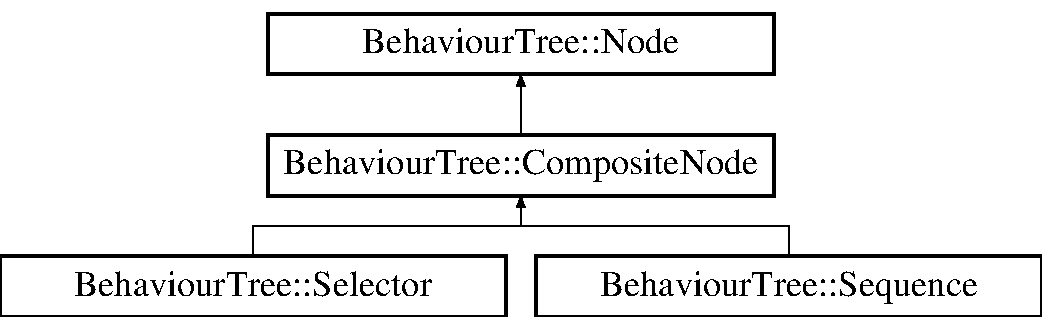
\includegraphics[height=3.000000cm]{class_behaviour_tree_1_1_composite_node}
\end{center}
\end{figure}
\subsection*{Public Member Functions}
\begin{DoxyCompactItemize}
\item 
\mbox{\Hypertarget{class_behaviour_tree_1_1_composite_node_a30dc5790c2ac65a7afd2311a071b15aa}\label{class_behaviour_tree_1_1_composite_node_a30dc5790c2ac65a7afd2311a071b15aa}} 
const std\+::vector$<$ \hyperlink{class_behaviour_tree_1_1_node}{Node} $\ast$ $>$ \& {\bfseries get\+Children} () const
\item 
\mbox{\Hypertarget{class_behaviour_tree_1_1_composite_node_a4ca3dcdd5bbe613d8f251a619a3240ba}\label{class_behaviour_tree_1_1_composite_node_a4ca3dcdd5bbe613d8f251a619a3240ba}} 
void {\bfseries add\+Child} (\hyperlink{class_behaviour_tree_1_1_node}{Node} $\ast$child)
\item 
\mbox{\Hypertarget{class_behaviour_tree_1_1_composite_node_a98d1b1bd7079079e89c9e10439928e24}\label{class_behaviour_tree_1_1_composite_node_a98d1b1bd7079079e89c9e10439928e24}} 
void {\bfseries add\+Children} (std\+::initializer\+\_\+list$<$ \hyperlink{class_behaviour_tree_1_1_node}{Node} $\ast$$>$ \&\&new\+Children)
\item 
\mbox{\Hypertarget{class_behaviour_tree_1_1_composite_node_ac2289d771089181e6bd4c7867ec21364}\label{class_behaviour_tree_1_1_composite_node_ac2289d771089181e6bd4c7867ec21364}} 
{\footnotesize template$<$typename C\+O\+N\+T\+A\+I\+N\+ER $>$ }\\void {\bfseries add\+Children} (const C\+O\+N\+T\+A\+I\+N\+ER \&new\+Children)
\end{DoxyCompactItemize}
\subsection*{Protected Member Functions}
\begin{DoxyCompactItemize}
\item 
\mbox{\Hypertarget{class_behaviour_tree_1_1_composite_node_ad8ac82a2cae0640b712873202bd4df49}\label{class_behaviour_tree_1_1_composite_node_ad8ac82a2cae0640b712873202bd4df49}} 
std\+::vector$<$ \hyperlink{class_behaviour_tree_1_1_node}{Node} $\ast$ $>$ {\bfseries children\+Shuffled} () const
\end{DoxyCompactItemize}


The documentation for this class was generated from the following file\+:\begin{DoxyCompactItemize}
\item 
C\+:/\+Users/\+Alastair/\+Documents/\+Git\+Hub/comp250-\/\+A\+I-\/portfolio/\+Space\+Game/\+S\+D\+L\+\_\+project/Behaviour\+Tree.\+h\end{DoxyCompactItemize}

\hypertarget{class_docking_doors}{}\section{Docking\+Doors Class Reference}
\label{class_docking_doors}\index{Docking\+Doors@{Docking\+Doors}}
\subsection*{Public Member Functions}
\begin{DoxyCompactItemize}
\item 
\mbox{\Hypertarget{class_docking_doors_a3e63df84955a9fbbdf0db9f30d63b60e}\label{class_docking_doors_a3e63df84955a9fbbdf0db9f30d63b60e}} 
void {\bfseries place\+Docking\+Doors} (S\+D\+L\+\_\+\+Renderer $\ast$renderer, \hyperlink{class_level}{Level} \&level)
\item 
\mbox{\Hypertarget{class_docking_doors_a0cacbcddb4ba243e2e74bfbe5c51e3aa}\label{class_docking_doors_a0cacbcddb4ba243e2e74bfbe5c51e3aa}} 
void {\bfseries change\+Orientation} ()
\item 
\mbox{\Hypertarget{class_docking_doors_a17e2c587398f28d66ed57deaae79f3d8}\label{class_docking_doors_a17e2c587398f28d66ed57deaae79f3d8}} 
void {\bfseries render\+Overlay} (S\+D\+L\+\_\+\+Renderer $\ast$renderer, \hyperlink{class_level}{Level} \&level)
\item 
\mbox{\Hypertarget{class_docking_doors_affcb5dbe205755dbbeca3ead5c0c433b}\label{class_docking_doors_affcb5dbe205755dbbeca3ead5c0c433b}} 
void {\bfseries place\+Entry\+Path} (\hyperlink{class_level}{Level} \&level, int orientation)
\item 
\mbox{\Hypertarget{class_docking_doors_a6b4075011d18f7fc8dd66d7f71e50905}\label{class_docking_doors_a6b4075011d18f7fc8dd66d7f71e50905}} 
void {\bfseries place\+Airlock\+Door} (\hyperlink{class_level}{Level} \&level, int x, int y, int mouseY)
\end{DoxyCompactItemize}
\subsection*{Public Attributes}
\begin{DoxyCompactItemize}
\item 
\mbox{\Hypertarget{class_docking_doors_a7b0ebae2b928f2a790a6c04d0fafadeb}\label{class_docking_doors_a7b0ebae2b928f2a790a6c04d0fafadeb}} 
\hyperlink{class_texture}{Texture} {\bfseries overlay\+Texture}
\item 
\mbox{\Hypertarget{class_docking_doors_ae7db99081fa2d5865b3dead8f41eeb0e}\label{class_docking_doors_ae7db99081fa2d5865b3dead8f41eeb0e}} 
int {\bfseries dock\+Orientation} = 0
\item 
\mbox{\Hypertarget{class_docking_doors_a9d2ddca623a6798c1d820375a3d77691}\label{class_docking_doors_a9d2ddca623a6798c1d820375a3d77691}} 
bool {\bfseries place\+Only\+Once} = true
\end{DoxyCompactItemize}


The documentation for this class was generated from the following files\+:\begin{DoxyCompactItemize}
\item 
C\+:/\+Users/\+Alastair/\+Documents/\+Git\+Hub/comp250-\/\+A\+I-\/portfolio/\+Space\+Game/\+S\+D\+L\+\_\+project/Docking\+Doors.\+h\item 
C\+:/\+Users/\+Alastair/\+Documents/\+Git\+Hub/comp250-\/\+A\+I-\/portfolio/\+Space\+Game/\+S\+D\+L\+\_\+project/Docking\+Doors.\+cpp\end{DoxyCompactItemize}

\hypertarget{class_escape_menu}{}\section{Escape\+Menu Class Reference}
\label{class_escape_menu}\index{Escape\+Menu@{Escape\+Menu}}
\subsection*{Public Member Functions}
\begin{DoxyCompactItemize}
\item 
\mbox{\Hypertarget{class_escape_menu_ae40100baf65d9a897816046b8ddbf97c}\label{class_escape_menu_ae40100baf65d9a897816046b8ddbf97c}} 
void {\bfseries Run\+Escape\+Menu} (S\+D\+L\+\_\+\+Renderer $\ast$renderer, int W\+I\+N\+D\+O\+W\+\_\+\+W\+I\+D\+TH, int W\+I\+N\+D\+O\+W\+\_\+\+H\+E\+I\+G\+HT, int mouse\+\_\+X, int mouse\+\_\+Y, bool running)
\end{DoxyCompactItemize}
\subsection*{Public Attributes}
\begin{DoxyCompactItemize}
\item 
\mbox{\Hypertarget{class_escape_menu_aa0b49300db0d5b0e4b4b0e4712725a02}\label{class_escape_menu_aa0b49300db0d5b0e4b4b0e4712725a02}} 
\hyperlink{class_texture}{Texture} \hyperlink{class_escape_menu_aa0b49300db0d5b0e4b4b0e4712725a02}{menu\+Background\+Texture}
\begin{DoxyCompactList}\small\item\em Is the texture for the menu background. \end{DoxyCompactList}\item 
\mbox{\Hypertarget{class_escape_menu_ada3116b5ec7d80e195aed9fa9c642079}\label{class_escape_menu_ada3116b5ec7d80e195aed9fa9c642079}} 
\hyperlink{class_texture}{Texture} \hyperlink{class_escape_menu_ada3116b5ec7d80e195aed9fa9c642079}{exit\+Button\+Texture}
\begin{DoxyCompactList}\small\item\em Is the texture for the exit button on the menu. \end{DoxyCompactList}\item 
\mbox{\Hypertarget{class_escape_menu_a6051b15974dbbd14b49c0979b5e73cdd}\label{class_escape_menu_a6051b15974dbbd14b49c0979b5e73cdd}} 
\hyperlink{class_texture}{Texture} \hyperlink{class_escape_menu_a6051b15974dbbd14b49c0979b5e73cdd}{exit\+Button\+Highlighted}
\begin{DoxyCompactList}\small\item\em Is the texture for the highlited exit button. \end{DoxyCompactList}\item 
\mbox{\Hypertarget{class_escape_menu_a99d107c99bf01d58783dae4bb11e305a}\label{class_escape_menu_a99d107c99bf01d58783dae4bb11e305a}} 
\hyperlink{class_texture}{Texture} \hyperlink{class_escape_menu_a99d107c99bf01d58783dae4bb11e305a}{restart\+Button\+Texture}
\begin{DoxyCompactList}\small\item\em Is the texture for the restart button. \end{DoxyCompactList}\item 
\mbox{\Hypertarget{class_escape_menu_a5020fd89d63f51edb353853920c0892f}\label{class_escape_menu_a5020fd89d63f51edb353853920c0892f}} 
\hyperlink{class_texture}{Texture} \hyperlink{class_escape_menu_a5020fd89d63f51edb353853920c0892f}{restart\+Button\+Highlighted}
\begin{DoxyCompactList}\small\item\em Is the texuture for the highlighted restart button. \end{DoxyCompactList}\item 
\mbox{\Hypertarget{class_escape_menu_ae7d75c060778703ea8a2d62cb786932f}\label{class_escape_menu_ae7d75c060778703ea8a2d62cb786932f}} 
bool {\bfseries restart} = false
\item 
\mbox{\Hypertarget{class_escape_menu_a7c518ab405d235a17014845a933259a1}\label{class_escape_menu_a7c518ab405d235a17014845a933259a1}} 
bool {\bfseries exit} = false
\end{DoxyCompactItemize}


The documentation for this class was generated from the following files\+:\begin{DoxyCompactItemize}
\item 
C\+:/\+Users/\+Alastair/\+Documents/\+Git\+Hub/comp250-\/\+A\+I-\/portfolio/\+Space\+Game/\+S\+D\+L\+\_\+project/Escape\+Menu.\+h\item 
C\+:/\+Users/\+Alastair/\+Documents/\+Git\+Hub/comp250-\/\+A\+I-\/portfolio/\+Space\+Game/\+S\+D\+L\+\_\+project/Escape\+Menu.\+cpp\end{DoxyCompactItemize}

\hypertarget{class_fire}{}\section{Fire Class Reference}
\label{class_fire}\index{Fire@{Fire}}
\subsection*{Public Member Functions}
\begin{DoxyCompactItemize}
\item 
\mbox{\Hypertarget{class_fire_af18ee6c1bed8ecf145daeeb56708b039}\label{class_fire_af18ee6c1bed8ecf145daeeb56708b039}} 
void \hyperlink{class_fire_af18ee6c1bed8ecf145daeeb56708b039}{fire\+Spread} (\hyperlink{class_level}{Level} \&grid, int cellX, int cellY)
\begin{DoxyCompactList}\small\item\em Determines how the fire will spread. \end{DoxyCompactList}\item 
\mbox{\Hypertarget{class_fire_a15f3123eb1d1afd3d4937a3287b9dc35}\label{class_fire_a15f3123eb1d1afd3d4937a3287b9dc35}} 
void \hyperlink{class_fire_a15f3123eb1d1afd3d4937a3287b9dc35}{spawn} (\hyperlink{class_level}{Level} \&grid, int cellX, int cellY)
\begin{DoxyCompactList}\small\item\em Spawns the fire at level start. \end{DoxyCompactList}\item 
\mbox{\Hypertarget{class_fire_acd45932783d247f80e4f2d2a043b4508}\label{class_fire_acd45932783d247f80e4f2d2a043b4508}} 
void \hyperlink{class_fire_acd45932783d247f80e4f2d2a043b4508}{fire\+Extinguisher} ()
\begin{DoxyCompactList}\small\item\em manages the fire extinguisher \end{DoxyCompactList}\end{DoxyCompactItemize}
\subsection*{Public Attributes}
\begin{DoxyCompactItemize}
\item 
\mbox{\Hypertarget{class_fire_acb6bb3c895c92c8ac03595b6f8962ba0}\label{class_fire_acb6bb3c895c92c8ac03595b6f8962ba0}} 
unsigned int \hyperlink{class_fire_acb6bb3c895c92c8ac03595b6f8962ba0}{last\+Time} = 0
\begin{DoxyCompactList}\small\item\em Sets the time variables. \end{DoxyCompactList}\item 
\mbox{\Hypertarget{class_fire_ae62b26ad098d04b06bf873925995e284}\label{class_fire_ae62b26ad098d04b06bf873925995e284}} 
unsigned int {\bfseries current\+Time}
\item 
\mbox{\Hypertarget{class_fire_a9a0d858289975b93c3dc729d9b75cf95}\label{class_fire_a9a0d858289975b93c3dc729d9b75cf95}} 
float \hyperlink{class_fire_a9a0d858289975b93c3dc729d9b75cf95}{firespawntimer} = 1000
\begin{DoxyCompactList}\small\item\em time in seconds that fire will spawn \end{DoxyCompactList}\end{DoxyCompactItemize}


The documentation for this class was generated from the following files\+:\begin{DoxyCompactItemize}
\item 
C\+:/\+Users/\+Alastair/\+Documents/\+Git\+Hub/comp250-\/\+A\+I-\/portfolio/\+Space\+Game/\+S\+D\+L\+\_\+project/Fire.\+h\item 
C\+:/\+Users/\+Alastair/\+Documents/\+Git\+Hub/comp250-\/\+A\+I-\/portfolio/\+Space\+Game/\+S\+D\+L\+\_\+project/Fire.\+cpp\end{DoxyCompactItemize}

\hypertarget{class_game_settings}{}\section{Game\+Settings Class Reference}
\label{class_game_settings}\index{Game\+Settings@{Game\+Settings}}
\subsection*{Public Member Functions}
\begin{DoxyCompactItemize}
\item 
\mbox{\Hypertarget{class_game_settings_a0021dbf029d3928a6b136fdc5df25e59}\label{class_game_settings_a0021dbf029d3928a6b136fdc5df25e59}} 
void {\bfseries get\+Screen\+Resolution} ()
\end{DoxyCompactItemize}
\subsection*{Public Attributes}
\begin{DoxyCompactItemize}
\item 
\mbox{\Hypertarget{class_game_settings_a08bd6d169f42dac744c792bfc4c2118e}\label{class_game_settings_a08bd6d169f42dac744c792bfc4c2118e}} 
const int \hyperlink{class_game_settings_a08bd6d169f42dac744c792bfc4c2118e}{F\+R\+A\+M\+E\+\_\+\+R\+A\+TE} = 60
\begin{DoxyCompactList}\small\item\em int that will be used to control movement speed \end{DoxyCompactList}\item 
\mbox{\Hypertarget{class_game_settings_ad7ab595cc408853b20ac98b064fd9272}\label{class_game_settings_ad7ab595cc408853b20ac98b064fd9272}} 
int \hyperlink{class_game_settings_ad7ab595cc408853b20ac98b064fd9272}{W\+I\+N\+D\+O\+W\+\_\+\+W\+I\+D\+TH} = 800
\begin{DoxyCompactList}\small\item\em initial window settings \end{DoxyCompactList}\item 
\mbox{\Hypertarget{class_game_settings_a87eb5f9c3d55aabe1780871b0005cbf9}\label{class_game_settings_a87eb5f9c3d55aabe1780871b0005cbf9}} 
int {\bfseries W\+I\+N\+D\+O\+W\+\_\+\+H\+E\+I\+G\+HT} = 600
\item 
\mbox{\Hypertarget{class_game_settings_ac38e368e94d990cde54d8b0c0dca65de}\label{class_game_settings_ac38e368e94d990cde54d8b0c0dca65de}} 
bool {\bfseries fullscreen} = false
\item 
\mbox{\Hypertarget{class_game_settings_a71c452d4138b06276d7825047a654bc0}\label{class_game_settings_a71c452d4138b06276d7825047a654bc0}} 
S\+D\+L\+\_\+\+Display\+Mode \hyperlink{class_game_settings_a71c452d4138b06276d7825047a654bc0}{current\+Display}
\begin{DoxyCompactList}\small\item\em stores screen resolution \end{DoxyCompactList}\end{DoxyCompactItemize}


The documentation for this class was generated from the following files\+:\begin{DoxyCompactItemize}
\item 
C\+:/\+Users/\+Alastair/\+Documents/\+Git\+Hub/comp250-\/\+A\+I-\/portfolio/\+Space\+Game/\+S\+D\+L\+\_\+project/Game\+Settings.\+h\item 
C\+:/\+Users/\+Alastair/\+Documents/\+Git\+Hub/comp250-\/\+A\+I-\/portfolio/\+Space\+Game/\+S\+D\+L\+\_\+project/Game\+Settings.\+cpp\end{DoxyCompactItemize}

\hypertarget{class_g_u_i}{}\section{G\+UI Class Reference}
\label{class_g_u_i}\index{G\+UI@{G\+UI}}
Inheritance diagram for G\+UI\+:\begin{figure}[H]
\begin{center}
\leavevmode
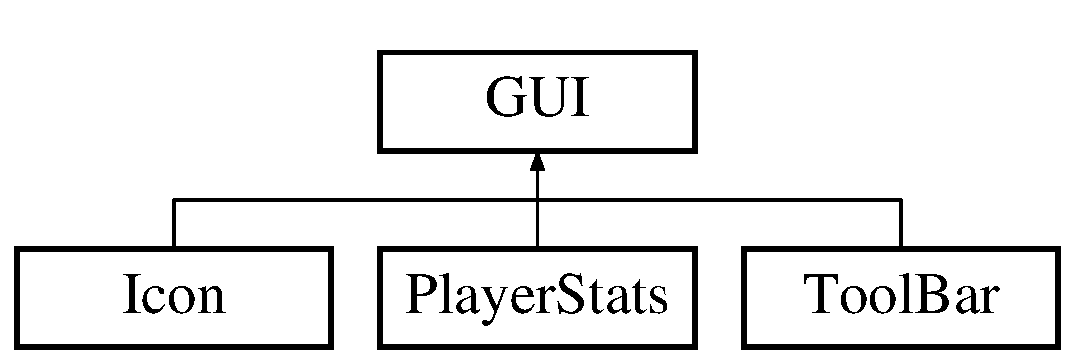
\includegraphics[height=2.000000cm]{class_g_u_i}
\end{center}
\end{figure}
\subsection*{Public Member Functions}
\begin{DoxyCompactItemize}
\item 
\mbox{\Hypertarget{class_g_u_i_a84f72298745c32d42cff88122f064b87}\label{class_g_u_i_a84f72298745c32d42cff88122f064b87}} 
int {\bfseries getX} ()
\item 
\mbox{\Hypertarget{class_g_u_i_a6092c145d73a1ba90b363413994ed1c2}\label{class_g_u_i_a6092c145d73a1ba90b363413994ed1c2}} 
int {\bfseries getY} ()
\item 
\mbox{\Hypertarget{class_g_u_i_a1ea78c6d2cd7527949c86d6364e0ba58}\label{class_g_u_i_a1ea78c6d2cd7527949c86d6364e0ba58}} 
int {\bfseries setX} (int newX)
\item 
\mbox{\Hypertarget{class_g_u_i_a6a8fd57ede00d6ce473a5ca62dbe8c7c}\label{class_g_u_i_a6a8fd57ede00d6ce473a5ca62dbe8c7c}} 
int {\bfseries setY} (int newY)
\item 
\mbox{\Hypertarget{class_g_u_i_adf5b1e95c3b7993ffc260819d3b65a86}\label{class_g_u_i_adf5b1e95c3b7993ffc260819d3b65a86}} 
int {\bfseries get\+Width} ()
\item 
\mbox{\Hypertarget{class_g_u_i_a840bc57fdf153af9c3e6cd963de1c0d2}\label{class_g_u_i_a840bc57fdf153af9c3e6cd963de1c0d2}} 
int {\bfseries get\+Height} ()
\item 
\mbox{\Hypertarget{class_g_u_i_aded24bcc960ca3ff7679cf0deda9c2ec}\label{class_g_u_i_aded24bcc960ca3ff7679cf0deda9c2ec}} 
int {\bfseries set\+Width} (int new\+Width)
\item 
\mbox{\Hypertarget{class_g_u_i_a909f92c2f9553b8ff2b994b6559108d0}\label{class_g_u_i_a909f92c2f9553b8ff2b994b6559108d0}} 
int {\bfseries set\+Height} (int new\+Height)
\end{DoxyCompactItemize}


The documentation for this class was generated from the following files\+:\begin{DoxyCompactItemize}
\item 
C\+:/\+Users/\+Alastair/\+Documents/\+Git\+Hub/comp250-\/\+A\+I-\/portfolio/\+Space\+Game/\+S\+D\+L\+\_\+project/G\+U\+I.\+h\item 
C\+:/\+Users/\+Alastair/\+Documents/\+Git\+Hub/comp250-\/\+A\+I-\/portfolio/\+Space\+Game/\+S\+D\+L\+\_\+project/G\+U\+I.\+cpp\end{DoxyCompactItemize}

\hypertarget{class_hydroponics}{}\section{Hydroponics Class Reference}
\label{class_hydroponics}\index{Hydroponics@{Hydroponics}}
Inheritance diagram for Hydroponics\+:\begin{figure}[H]
\begin{center}
\leavevmode
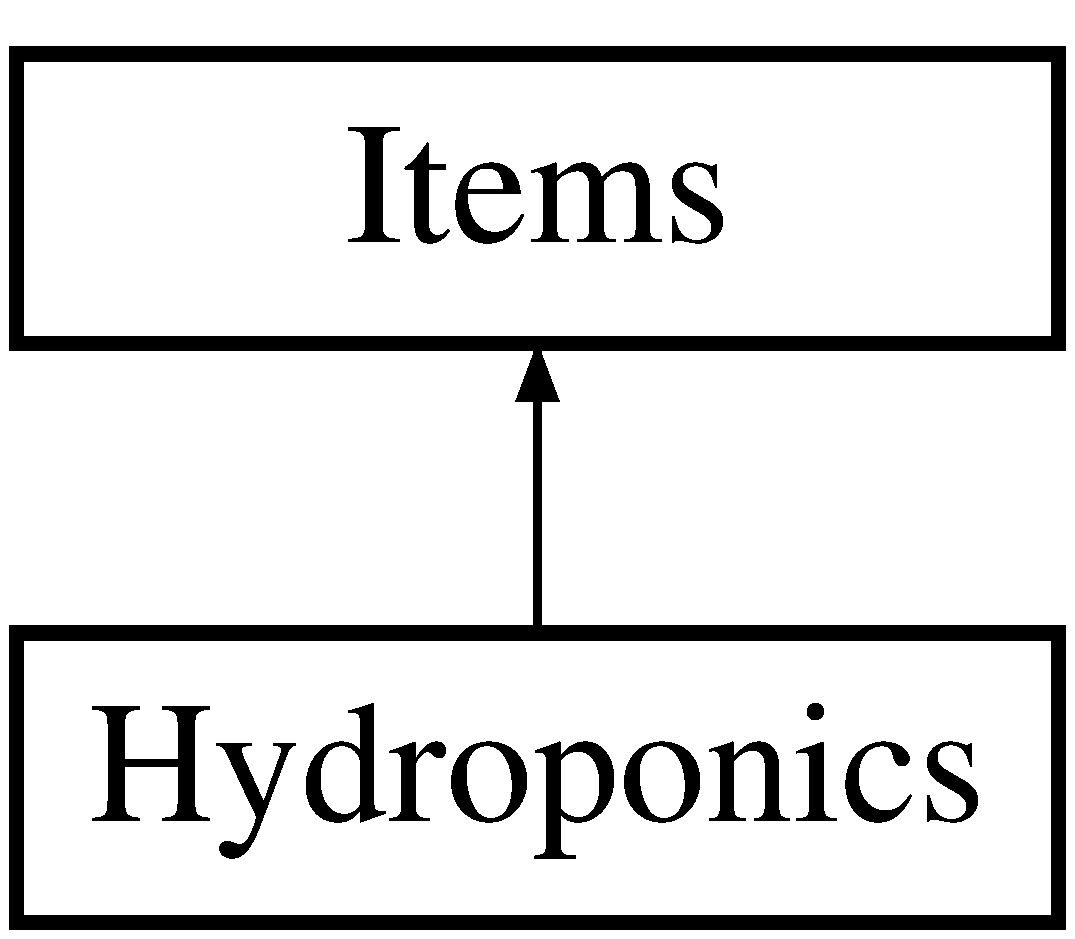
\includegraphics[height=2.000000cm]{class_hydroponics}
\end{center}
\end{figure}
\subsection*{Public Member Functions}
\begin{DoxyCompactItemize}
\item 
\mbox{\Hypertarget{class_hydroponics_a596222f47012d8452cc9e5d63ed64fda}\label{class_hydroponics_a596222f47012d8452cc9e5d63ed64fda}} 
void {\bfseries render\+Items} (S\+D\+L\+\_\+\+Renderer $\ast$renderer, \hyperlink{class_level}{Level} \&level, std\+::vector$<$ \hyperlink{class_hydroponics}{Hydroponics} $>$ \&all\+Hydroponics\+Farms)
\item 
\mbox{\Hypertarget{class_hydroponics_afd257a941472c8fe73fb45aaeda516d1}\label{class_hydroponics_afd257a941472c8fe73fb45aaeda516d1}} 
void {\bfseries update} (\hyperlink{class_level}{Level} \&level, std\+::vector$<$ \hyperlink{class_hydroponics}{Hydroponics} $>$ \&all\+Hydroponics\+Farms, int \&x, int \&y)
\item 
\mbox{\Hypertarget{class_hydroponics_ae997320fac01b8da96ae3e70458c0a02}\label{class_hydroponics_ae997320fac01b8da96ae3e70458c0a02}} 
void {\bfseries spawn\+Hydroponic\+Base} (S\+D\+L\+\_\+\+Renderer $\ast$renderer, \hyperlink{class_level}{Level} \&level, std\+::vector$<$ \hyperlink{class_hydroponics}{Hydroponics} $>$ \&all\+Hydroponics\+Farms, int x, int y)
\end{DoxyCompactItemize}
\subsection*{Public Attributes}
\begin{DoxyCompactItemize}
\item 
\mbox{\Hypertarget{class_hydroponics_af94045fbbcb208b332d95bb712135056}\label{class_hydroponics_af94045fbbcb208b332d95bb712135056}} 
bool {\bfseries is\+Producing\+Oxygen} = true
\item 
\mbox{\Hypertarget{class_hydroponics_ab33b17ae6e1f74fb62093f99632338fc}\label{class_hydroponics_ab33b17ae6e1f74fb62093f99632338fc}} 
bool {\bfseries is\+Producing\+Food} = true
\item 
\mbox{\Hypertarget{class_hydroponics_a8cd445b84d3227cb39a2f5255d3002e6}\label{class_hydroponics_a8cd445b84d3227cb39a2f5255d3002e6}} 
bool {\bfseries is\+Hydroponics} = true
\item 
\mbox{\Hypertarget{class_hydroponics_a5496629c4a016c3ad9d35f3fcb7715d8}\label{class_hydroponics_a5496629c4a016c3ad9d35f3fcb7715d8}} 
\hyperlink{class_texture}{Texture} \hyperlink{class_hydroponics_a5496629c4a016c3ad9d35f3fcb7715d8}{hydroponics\+Texture}
\begin{DoxyCompactList}\small\item\em \hyperlink{class_texture}{Texture} for hydroponics. \end{DoxyCompactList}\item 
\mbox{\Hypertarget{class_hydroponics_aa865e914472935719c7cb9f559478100}\label{class_hydroponics_aa865e914472935719c7cb9f559478100}} 
\hyperlink{class_texture}{Texture} {\bfseries left\+Hydroponics}
\item 
\mbox{\Hypertarget{class_hydroponics_a511bf34c1b907164d61394b6ab8dd32a}\label{class_hydroponics_a511bf34c1b907164d61394b6ab8dd32a}} 
\hyperlink{class_texture}{Texture} {\bfseries center\+Hydroponics}
\item 
\mbox{\Hypertarget{class_hydroponics_a8ad23d4cdc2f8e9188295143210a963f}\label{class_hydroponics_a8ad23d4cdc2f8e9188295143210a963f}} 
\hyperlink{class_texture}{Texture} {\bfseries right\+Hydroponics}
\item 
\mbox{\Hypertarget{class_hydroponics_ac21b247254d6b4af3746ea38e54100c9}\label{class_hydroponics_ac21b247254d6b4af3746ea38e54100c9}} 
std\+::string {\bfseries Orientation} = \char`\"{}NA\char`\"{}
\item 
\mbox{\Hypertarget{class_hydroponics_aea1f52620240261ad02b156051d31694}\label{class_hydroponics_aea1f52620240261ad02b156051d31694}} 
double {\bfseries amount\+Of\+Oxygen\+Producing} = 0.\+1
\end{DoxyCompactItemize}


The documentation for this class was generated from the following files\+:\begin{DoxyCompactItemize}
\item 
C\+:/\+Users/\+Alastair/\+Documents/\+Git\+Hub/comp250-\/\+A\+I-\/portfolio/\+Space\+Game/\+S\+D\+L\+\_\+project/Hydroponics.\+h\item 
C\+:/\+Users/\+Alastair/\+Documents/\+Git\+Hub/comp250-\/\+A\+I-\/portfolio/\+Space\+Game/\+S\+D\+L\+\_\+project/Hydroponics.\+cpp\end{DoxyCompactItemize}

\hypertarget{class_icon}{}\section{Icon Class Reference}
\label{class_icon}\index{Icon@{Icon}}
Inheritance diagram for Icon\+:\begin{figure}[H]
\begin{center}
\leavevmode
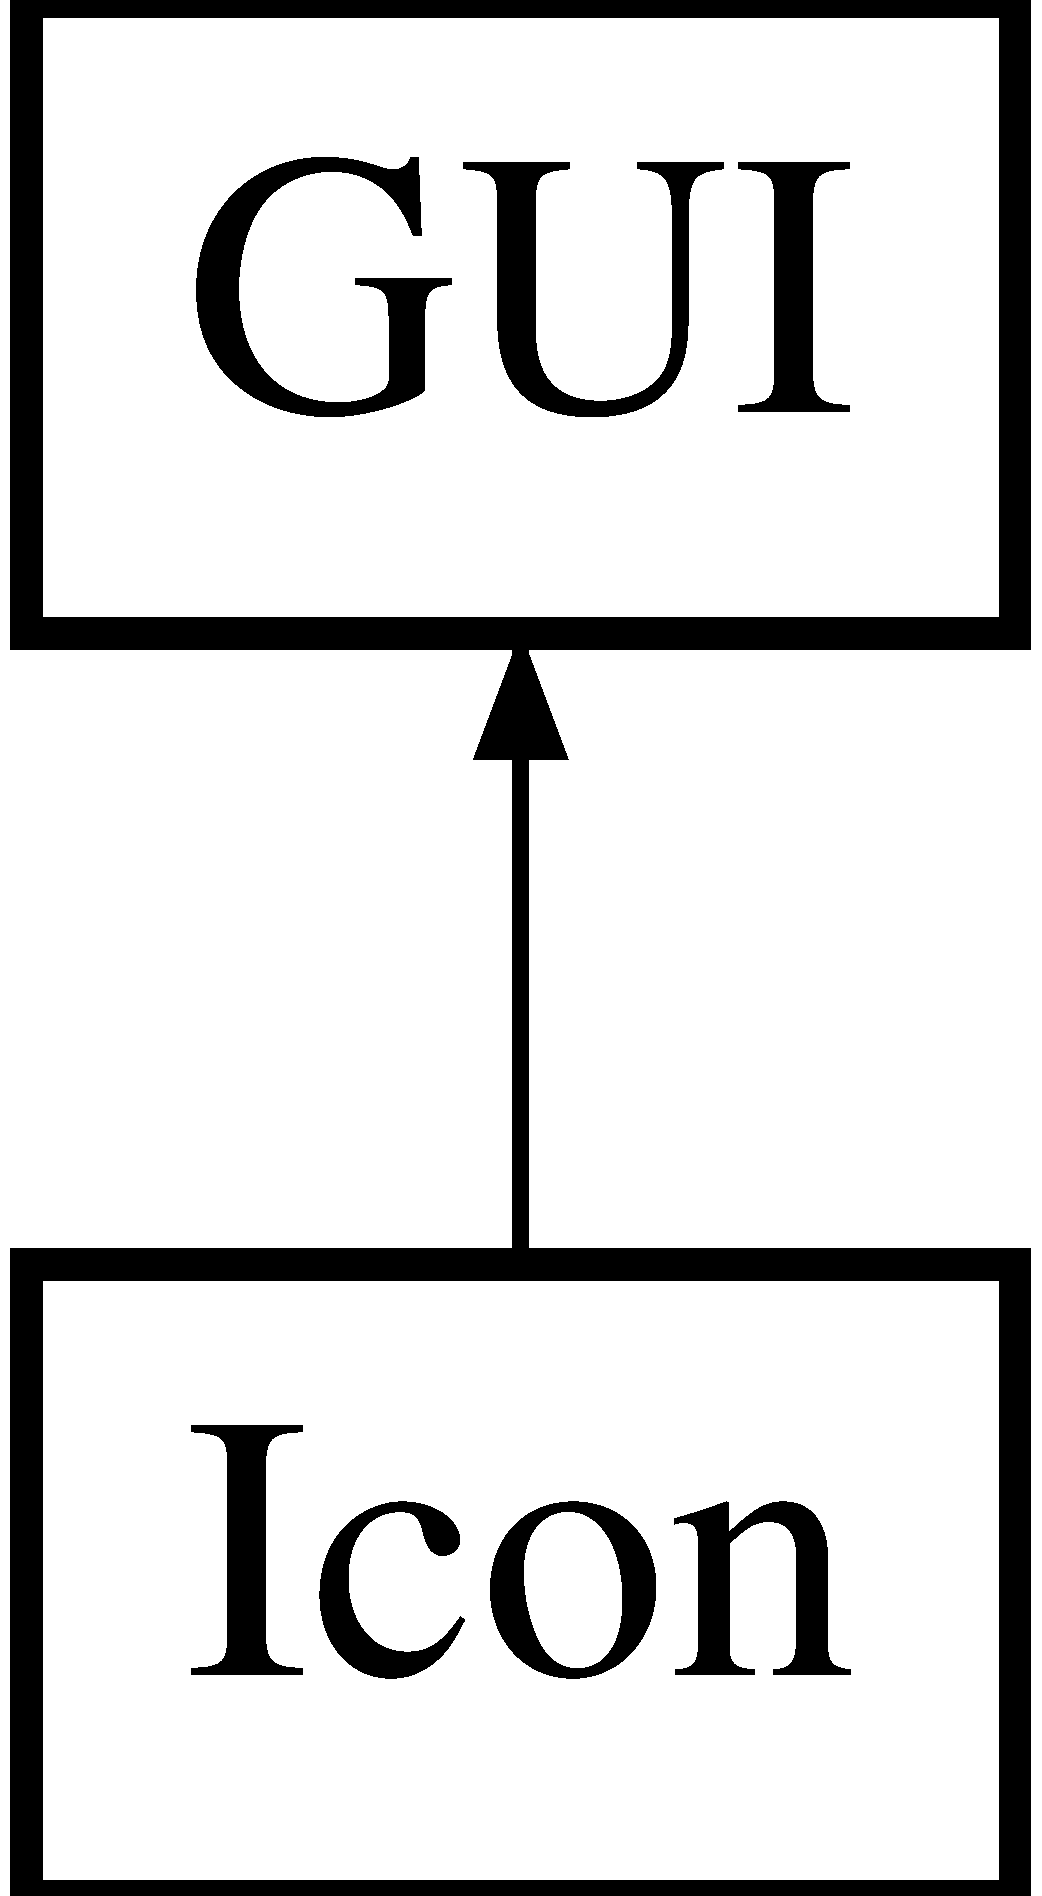
\includegraphics[height=2.000000cm]{class_icon}
\end{center}
\end{figure}
\subsection*{Public Member Functions}
\begin{DoxyCompactItemize}
\item 
\mbox{\Hypertarget{class_icon_a2c06009b9034912dea464e9f3c3791f9}\label{class_icon_a2c06009b9034912dea464e9f3c3791f9}} 
\hyperlink{class_icon_a2c06009b9034912dea464e9f3c3791f9}{Icon} ()
\begin{DoxyCompactList}\small\item\em Constructor. \end{DoxyCompactList}\item 
\mbox{\Hypertarget{class_icon_adb1b98ed12cd965ce849667c751e10c2}\label{class_icon_adb1b98ed12cd965ce849667c751e10c2}} 
\hyperlink{class_icon_adb1b98ed12cd965ce849667c751e10c2}{$\sim$\+Icon} ()
\begin{DoxyCompactList}\small\item\em Destructor. \end{DoxyCompactList}\item 
\mbox{\Hypertarget{class_icon_a33eff58279320449d77be043be5625b1}\label{class_icon_a33eff58279320449d77be043be5625b1}} 
int {\bfseries get\+Icon\+ID} ()
\item 
\mbox{\Hypertarget{class_icon_a278887be01cbb69175cb58f9ecf69894}\label{class_icon_a278887be01cbb69175cb58f9ecf69894}} 
int {\bfseries set\+Icon\+ID} (int new\+Icon\+ID)
\end{DoxyCompactItemize}


The documentation for this class was generated from the following files\+:\begin{DoxyCompactItemize}
\item 
C\+:/\+Users/\+Alastair/\+Documents/\+Git\+Hub/comp250-\/\+A\+I-\/portfolio/\+Space\+Game/\+S\+D\+L\+\_\+project/Icon.\+h\item 
C\+:/\+Users/\+Alastair/\+Documents/\+Git\+Hub/comp250-\/\+A\+I-\/portfolio/\+Space\+Game/\+S\+D\+L\+\_\+project/Icon.\+cpp\end{DoxyCompactItemize}

\hypertarget{class_initialisation_error}{}\section{Initialisation\+Error Class Reference}
\label{class_initialisation_error}\index{Initialisation\+Error@{Initialisation\+Error}}
Inheritance diagram for Initialisation\+Error\+:\begin{figure}[H]
\begin{center}
\leavevmode
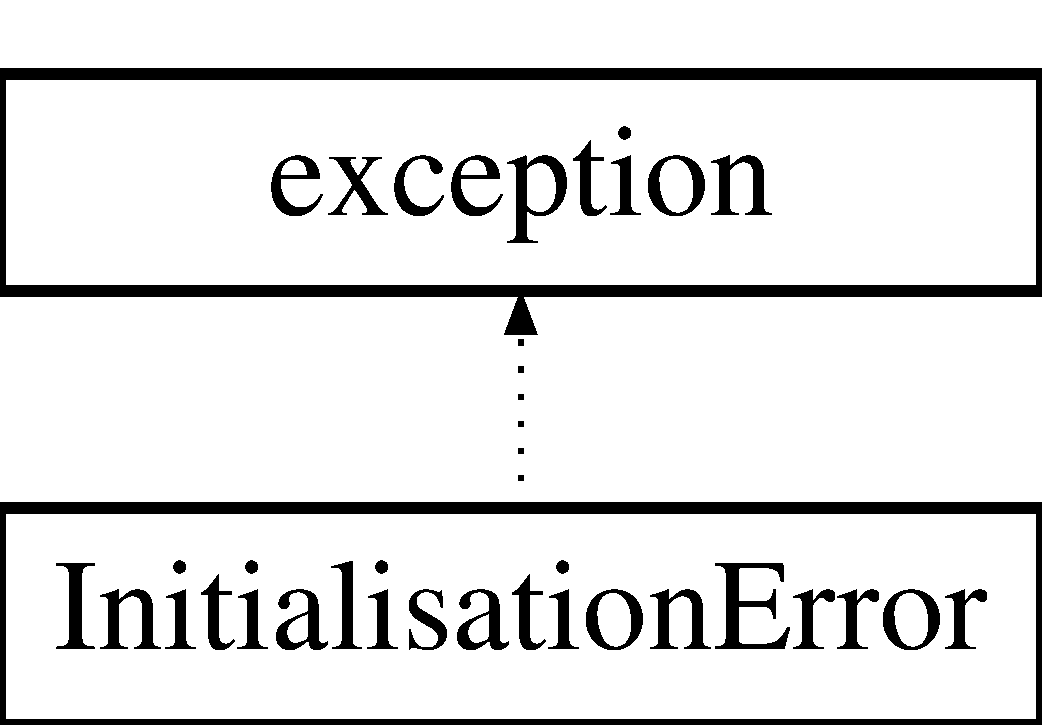
\includegraphics[height=2.000000cm]{class_initialisation_error}
\end{center}
\end{figure}
\subsection*{Public Member Functions}
\begin{DoxyCompactItemize}
\item 
\mbox{\Hypertarget{class_initialisation_error_ad3914b576cdb5ebffb1cee546167a769}\label{class_initialisation_error_ad3914b576cdb5ebffb1cee546167a769}} 
{\bfseries Initialisation\+Error} (const std\+::string \&msg)
\item 
\mbox{\Hypertarget{class_initialisation_error_afb7ca00778bc562ed3e763410c64ecfc}\label{class_initialisation_error_afb7ca00778bc562ed3e763410c64ecfc}} 
const char $\ast$ {\bfseries what} ()
\end{DoxyCompactItemize}


The documentation for this class was generated from the following files\+:\begin{DoxyCompactItemize}
\item 
C\+:/\+Users/\+Alastair/\+Documents/\+Git\+Hub/comp250-\/\+A\+I-\/portfolio/\+Space\+Game/\+S\+D\+L\+\_\+project/Initialisation\+Error.\+h\item 
C\+:/\+Users/\+Alastair/\+Documents/\+Git\+Hub/comp250-\/\+A\+I-\/portfolio/\+Space\+Game/\+S\+D\+L\+\_\+project/Initialisation\+Error.\+cpp\end{DoxyCompactItemize}

\hypertarget{class_items}{}\section{Items Class Reference}
\label{class_items}\index{Items@{Items}}
Inheritance diagram for Items\+:\begin{figure}[H]
\begin{center}
\leavevmode
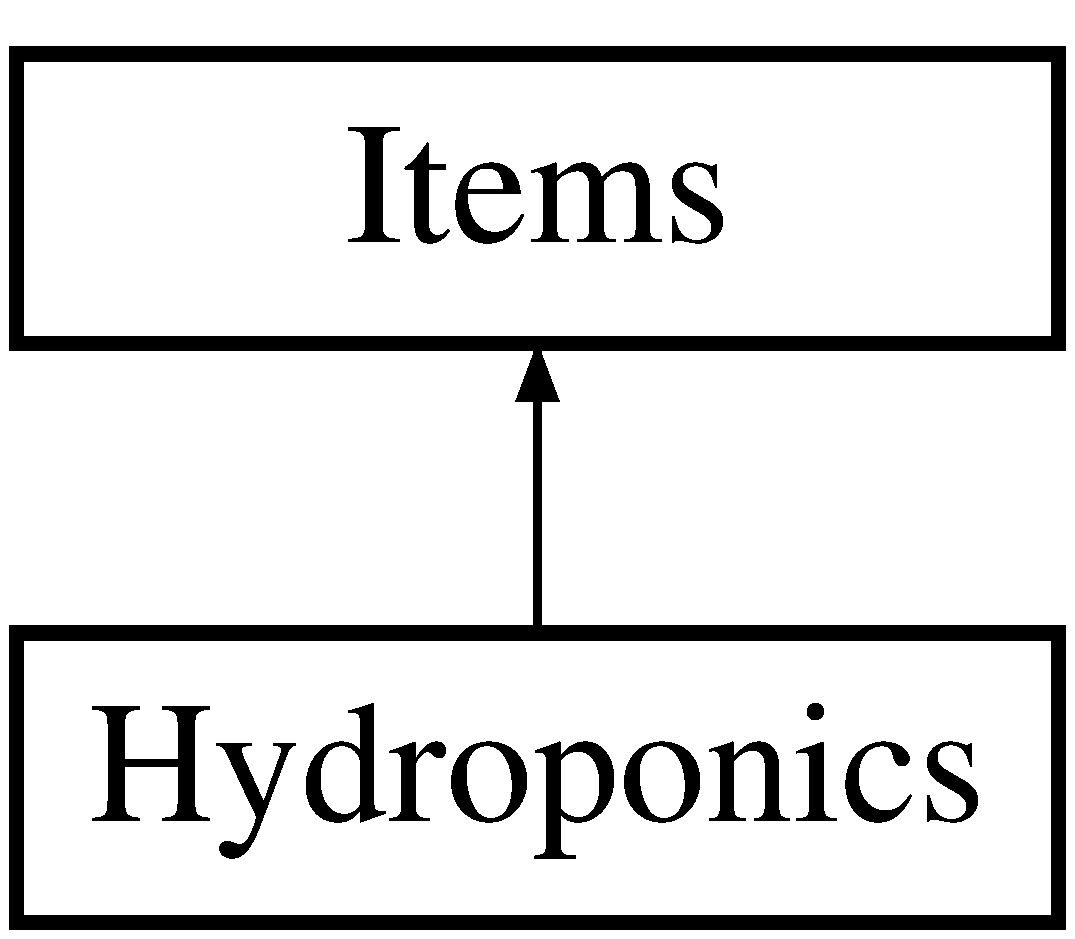
\includegraphics[height=2.000000cm]{class_items}
\end{center}
\end{figure}
\subsection*{Public Member Functions}
\begin{DoxyCompactItemize}
\item 
\mbox{\Hypertarget{class_items_a3d368c3c7a14eb2a038682bd4da5d41a}\label{class_items_a3d368c3c7a14eb2a038682bd4da5d41a}} 
\hyperlink{class_items_a3d368c3c7a14eb2a038682bd4da5d41a}{Items} ()
\begin{DoxyCompactList}\small\item\em Constructor. \end{DoxyCompactList}\item 
\mbox{\Hypertarget{class_items_acf985c70d843ae5e7adf65a528781cd5}\label{class_items_acf985c70d843ae5e7adf65a528781cd5}} 
\hyperlink{class_items_acf985c70d843ae5e7adf65a528781cd5}{$\sim$\+Items} ()
\begin{DoxyCompactList}\small\item\em Destructor. \end{DoxyCompactList}\item 
\mbox{\Hypertarget{class_items_ae7316fb789fc2c35cc9e50158fc5c676}\label{class_items_ae7316fb789fc2c35cc9e50158fc5c676}} 
int {\bfseries getX} ()
\item 
\mbox{\Hypertarget{class_items_ae540756a31ee087668437adfa0bcbabb}\label{class_items_ae540756a31ee087668437adfa0bcbabb}} 
int {\bfseries setX} (int newX)
\item 
\mbox{\Hypertarget{class_items_a669d8a09bd3b04aac1072045b2cd3906}\label{class_items_a669d8a09bd3b04aac1072045b2cd3906}} 
int {\bfseries getY} ()
\item 
\mbox{\Hypertarget{class_items_aa56c5ecfcff176613ef1a96d1c91d418}\label{class_items_aa56c5ecfcff176613ef1a96d1c91d418}} 
int {\bfseries setY} (int newY)
\item 
\mbox{\Hypertarget{class_items_a7b2f9eef38b7362c84af772bb89fbde7}\label{class_items_a7b2f9eef38b7362c84af772bb89fbde7}} 
int {\bfseries getwidth} ()
\item 
\mbox{\Hypertarget{class_items_ac4d3e7e149fe39d24b0e492fef3ea52b}\label{class_items_ac4d3e7e149fe39d24b0e492fef3ea52b}} 
int {\bfseries setwidth} (int newwidth)
\item 
\mbox{\Hypertarget{class_items_aab5dfe9d18f6a547dfa3a719d7f5bb0f}\label{class_items_aab5dfe9d18f6a547dfa3a719d7f5bb0f}} 
int {\bfseries getheight} ()
\item 
\mbox{\Hypertarget{class_items_a153af89dbbb17a4f424671907197bb9f}\label{class_items_a153af89dbbb17a4f424671907197bb9f}} 
int {\bfseries setheight} (int newheight)
\item 
\mbox{\Hypertarget{class_items_a0cdc283e37d8f8960ccfd06d57cd8468}\label{class_items_a0cdc283e37d8f8960ccfd06d57cd8468}} 
float {\bfseries get\+Health} ()
\item 
\mbox{\Hypertarget{class_items_a8c1844d384ae3785dbdfca56be94e15c}\label{class_items_a8c1844d384ae3785dbdfca56be94e15c}} 
float {\bfseries set\+Health} (int newhealth)
\end{DoxyCompactItemize}
\subsection*{Public Attributes}
\begin{DoxyCompactItemize}
\item 
\mbox{\Hypertarget{class_items_aabd80c6842ce11419edd5830d6e86e26}\label{class_items_aabd80c6842ce11419edd5830d6e86e26}} 
\hyperlink{class_level}{Level} {\bfseries level}
\end{DoxyCompactItemize}


The documentation for this class was generated from the following files\+:\begin{DoxyCompactItemize}
\item 
C\+:/\+Users/\+Alastair/\+Documents/\+Git\+Hub/comp250-\/\+A\+I-\/portfolio/\+Space\+Game/\+S\+D\+L\+\_\+project/Items.\+h\item 
C\+:/\+Users/\+Alastair/\+Documents/\+Git\+Hub/comp250-\/\+A\+I-\/portfolio/\+Space\+Game/\+S\+D\+L\+\_\+project/Items.\+cpp\end{DoxyCompactItemize}

\hypertarget{class_level}{}\section{Level Class Reference}
\label{class_level}\index{Level@{Level}}


This class generates the base of the level.  




{\ttfamily \#include $<$Level.\+h$>$}

\subsection*{Public Member Functions}
\begin{DoxyCompactItemize}
\item 
\mbox{\Hypertarget{class_level_a7a696c928ca5d5354db6e50e46d0f67d}\label{class_level_a7a696c928ca5d5354db6e50e46d0f67d}} 
\hyperlink{class_level_a7a696c928ca5d5354db6e50e46d0f67d}{Level} ()
\begin{DoxyCompactList}\small\item\em A constructor. \end{DoxyCompactList}\item 
\mbox{\Hypertarget{class_level_a249eac1e8f19ff44134efa5e986feaca}\label{class_level_a249eac1e8f19ff44134efa5e986feaca}} 
\hyperlink{class_level_a249eac1e8f19ff44134efa5e986feaca}{$\sim$\+Level} ()
\begin{DoxyCompactList}\small\item\em A deconstructor. \end{DoxyCompactList}\item 
\mbox{\Hypertarget{class_level_a0b6d16a7850bee00c1079ae6caa09658}\label{class_level_a0b6d16a7850bee00c1079ae6caa09658}} 
int \hyperlink{class_level_a0b6d16a7850bee00c1079ae6caa09658}{get\+Cell\+Size} ()
\begin{DoxyCompactList}\small\item\em Return the cell\+Size. \end{DoxyCompactList}\item 
\mbox{\Hypertarget{class_level_a097cc355bb986141ab1293b6326fc7dd}\label{class_level_a097cc355bb986141ab1293b6326fc7dd}} 
int {\bfseries set\+Cell\+Size} (int new\+Cell\+Size)
\item 
\mbox{\Hypertarget{class_level_a986cd05306bcdbb9f8e1dbddab258076}\label{class_level_a986cd05306bcdbb9f8e1dbddab258076}} 
int {\bfseries get\+Level\+Width} ()
\item 
\mbox{\Hypertarget{class_level_a78ab827c2c598cc5e9ae29af6617eee7}\label{class_level_a78ab827c2c598cc5e9ae29af6617eee7}} 
int {\bfseries get\+Level\+Height} ()
\item 
\mbox{\Hypertarget{class_level_a711767475094a647d934c11416adc732}\label{class_level_a711767475094a647d934c11416adc732}} 
void \hyperlink{class_level_a711767475094a647d934c11416adc732}{make\+Grid} (int Window\+\_\+\+Width, int Window\+\_\+\+Height)
\begin{DoxyCompactList}\small\item\em Fills grid with vectors of shared pointers to cells. \end{DoxyCompactList}\end{DoxyCompactItemize}
\subsection*{Public Attributes}
\begin{DoxyCompactItemize}
\item 
\mbox{\Hypertarget{class_level_a48cd01c916a30fa65a72ccca7ad79fe1}\label{class_level_a48cd01c916a30fa65a72ccca7ad79fe1}} 
std\+::vector$<$ std\+::vector$<$ std\+::shared\+\_\+ptr$<$ \hyperlink{class_cell}{Cell} $>$ $>$ $>$ \hyperlink{class_level_a48cd01c916a30fa65a72ccca7ad79fe1}{grid}
\begin{DoxyCompactList}\small\item\em The base grid that contains the cells. \end{DoxyCompactList}\end{DoxyCompactItemize}
\subsection*{Protected Attributes}
\begin{DoxyCompactItemize}
\item 
\mbox{\Hypertarget{class_level_a50fe4de705aaa281592ddc26c21362ec}\label{class_level_a50fe4de705aaa281592ddc26c21362ec}} 
int \hyperlink{class_level_a50fe4de705aaa281592ddc26c21362ec}{cell\+Size} = 50
\begin{DoxyCompactList}\small\item\em The size that the cell will be rendered at. \end{DoxyCompactList}\item 
\mbox{\Hypertarget{class_level_a96a0acf0f21c6d980f9b8c75f13b1672}\label{class_level_a96a0acf0f21c6d980f9b8c75f13b1672}} 
int {\bfseries level\+Width}
\item 
\mbox{\Hypertarget{class_level_a629c045305fc11af293d710df7cadc5e}\label{class_level_a629c045305fc11af293d710df7cadc5e}} 
int {\bfseries level\+Height}
\end{DoxyCompactItemize}


\subsection{Detailed Description}
This class generates the base of the level. 

This class creates a vector of vector of shared pointers to cells 

The documentation for this class was generated from the following files\+:\begin{DoxyCompactItemize}
\item 
C\+:/\+Users/\+Alastair/\+Documents/\+Git\+Hub/comp250-\/\+A\+I-\/portfolio/\+Space\+Game/\+S\+D\+L\+\_\+project/Level.\+h\item 
C\+:/\+Users/\+Alastair/\+Documents/\+Git\+Hub/comp250-\/\+A\+I-\/portfolio/\+Space\+Game/\+S\+D\+L\+\_\+project/Level.\+cpp\end{DoxyCompactItemize}

\hypertarget{class_map}{}\section{Map Class Reference}
\label{class_map}\index{Map@{Map}}


The Class that handlles the creation of rooms.  




{\ttfamily \#include $<$Map.\+h$>$}

\subsection*{Public Member Functions}
\begin{DoxyCompactItemize}
\item 
\mbox{\Hypertarget{class_map_a0f5ad0fd4563497b4214038cbca8b582}\label{class_map_a0f5ad0fd4563497b4214038cbca8b582}} 
\hyperlink{class_map_a0f5ad0fd4563497b4214038cbca8b582}{Map} ()
\begin{DoxyCompactList}\small\item\em A Constructor. \end{DoxyCompactList}\item 
\mbox{\Hypertarget{class_map_aa403fbe09394ccf39747588f5168e3b2}\label{class_map_aa403fbe09394ccf39747588f5168e3b2}} 
\hyperlink{class_map_aa403fbe09394ccf39747588f5168e3b2}{$\sim$\+Map} ()
\begin{DoxyCompactList}\small\item\em A Deconstructor. \end{DoxyCompactList}\item 
\mbox{\Hypertarget{class_map_a10bafffa9cb710fbd0c134c349e0f24f}\label{class_map_a10bafffa9cb710fbd0c134c349e0f24f}} 
int \hyperlink{class_map_a10bafffa9cb710fbd0c134c349e0f24f}{random} (int smallest\+Value, int largest\+Value)
\begin{DoxyCompactList}\small\item\em Generates a random integer. \end{DoxyCompactList}\item 
\mbox{\Hypertarget{class_map_a6837111691935c0cafaad3adfa726be8}\label{class_map_a6837111691935c0cafaad3adfa726be8}} 
void \hyperlink{class_map_a6837111691935c0cafaad3adfa726be8}{Load\+Map} (std\+::string filename, \hyperlink{class_level}{Level} room)
\begin{DoxyCompactList}\small\item\em Loads in a map from a txt file. \end{DoxyCompactList}\item 
\mbox{\Hypertarget{class_map_ac1ffbdcddb96eb103cd9d9947105dda3}\label{class_map_ac1ffbdcddb96eb103cd9d9947105dda3}} 
void \hyperlink{class_map_ac1ffbdcddb96eb103cd9d9947105dda3}{generate\+Map} (\hyperlink{class_level}{Level} level, \hyperlink{class_room_design}{Room\+Design} \&roomdesign)
\begin{DoxyCompactList}\small\item\em Randomly generates a map and modifies the level. \end{DoxyCompactList}\end{DoxyCompactItemize}


\subsection{Detailed Description}
The Class that handlles the creation of rooms. 

This class modifies the level class to make patterns out of the cells and turn them into rooms using all of it\textquotesingle{}s various functions. 

The documentation for this class was generated from the following files\+:\begin{DoxyCompactItemize}
\item 
C\+:/\+Users/\+Alastair/\+Documents/\+Git\+Hub/comp250-\/\+A\+I-\/portfolio/\+Space\+Game/\+S\+D\+L\+\_\+project/Map.\+h\item 
C\+:/\+Users/\+Alastair/\+Documents/\+Git\+Hub/comp250-\/\+A\+I-\/portfolio/\+Space\+Game/\+S\+D\+L\+\_\+project/Map.\+cpp\end{DoxyCompactItemize}

\hypertarget{class_node}{}\section{Node Class Reference}
\label{class_node}\index{Node@{Node}}
\subsection*{Public Member Functions}
\begin{DoxyCompactItemize}
\item 
\mbox{\Hypertarget{class_node_aa87c87fa68b0386513671f234c9ad06f}\label{class_node_aa87c87fa68b0386513671f234c9ad06f}} 
{\bfseries Node} (\hyperlink{class_point}{Point} \&point)
\item 
\mbox{\Hypertarget{class_node_a23a19f53dfbb18fec58cdac90de3d144}\label{class_node_a23a19f53dfbb18fec58cdac90de3d144}} 
{\bfseries Node} (int x, int y)
\end{DoxyCompactItemize}
\subsection*{Public Attributes}
\begin{DoxyCompactItemize}
\item 
\mbox{\Hypertarget{class_node_a86ddd28e833c1132e29a35b734673094}\label{class_node_a86ddd28e833c1132e29a35b734673094}} 
\hyperlink{class_point}{Point} {\bfseries point}
\item 
\mbox{\Hypertarget{class_node_a95314c432adbee13bcac6876597b21a7}\label{class_node_a95314c432adbee13bcac6876597b21a7}} 
Node\+Status {\bfseries status} = Node\+Status\+::\+None
\item 
\mbox{\Hypertarget{class_node_af93b606cf10abfe1766617ad9de59b01}\label{class_node_af93b606cf10abfe1766617ad9de59b01}} 
double {\bfseries g} = 0
\item 
\mbox{\Hypertarget{class_node_ae96fc081027353fbe793c35ea511116b}\label{class_node_ae96fc081027353fbe793c35ea511116b}} 
double {\bfseries h} = 0
\item 
\mbox{\Hypertarget{class_node_a41265f70ebb5a82514e68902efe44aee}\label{class_node_a41265f70ebb5a82514e68902efe44aee}} 
std\+::shared\+\_\+ptr$<$ \hyperlink{class_node}{Node} $>$ {\bfseries came\+From}
\end{DoxyCompactItemize}


The documentation for this class was generated from the following file\+:\begin{DoxyCompactItemize}
\item 
C\+:/\+Users/\+Alastair/\+Documents/\+Git\+Hub/comp250-\/\+A\+I-\/portfolio/\+Space\+Game/\+S\+D\+L\+\_\+project/Path\+Finder.\+h\end{DoxyCompactItemize}

\hypertarget{class_behaviour_tree_1_1_node}{}\section{Behaviour\+Tree\+:\+:Node Class Reference}
\label{class_behaviour_tree_1_1_node}\index{Behaviour\+Tree\+::\+Node@{Behaviour\+Tree\+::\+Node}}
Inheritance diagram for Behaviour\+Tree\+:\+:Node\+:\begin{figure}[H]
\begin{center}
\leavevmode
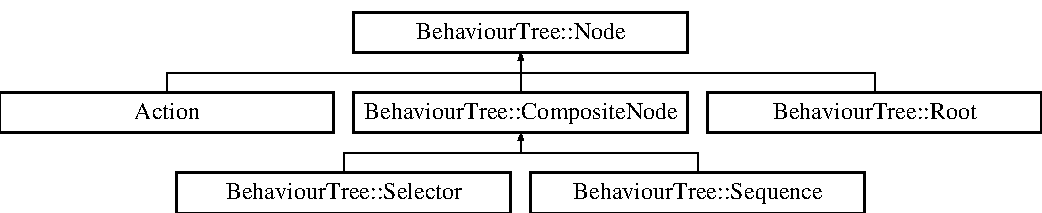
\includegraphics[height=2.828283cm]{class_behaviour_tree_1_1_node}
\end{center}
\end{figure}
\subsection*{Public Member Functions}
\begin{DoxyCompactItemize}
\item 
\mbox{\Hypertarget{class_behaviour_tree_1_1_node_a33b757627e0894459fa910443a15a44d}\label{class_behaviour_tree_1_1_node_a33b757627e0894459fa910443a15a44d}} 
virtual bool {\bfseries run} ()=0
\end{DoxyCompactItemize}


The documentation for this class was generated from the following file\+:\begin{DoxyCompactItemize}
\item 
C\+:/\+Users/\+Alastair/\+Documents/\+Git\+Hub/comp250-\/\+A\+I-\/portfolio/\+Space\+Game/\+S\+D\+L\+\_\+project/Behaviour\+Tree.\+h\end{DoxyCompactItemize}

\hypertarget{class_oxygen}{}\section{Oxygen Class Reference}
\label{class_oxygen}\index{Oxygen@{Oxygen}}


{\ttfamily \#include $<$Oxygen.\+h$>$}

\subsection*{Public Member Functions}
\begin{DoxyCompactItemize}
\item 
\mbox{\Hypertarget{class_oxygen_ac8c86509d4c1510faa526a65922d920e}\label{class_oxygen_ac8c86509d4c1510faa526a65922d920e}} 
\hyperlink{class_oxygen_ac8c86509d4c1510faa526a65922d920e}{Oxygen} ()
\begin{DoxyCompactList}\small\item\em A constructor. \end{DoxyCompactList}\item 
\mbox{\Hypertarget{class_oxygen_aca530b4693aa5ddc4c8b7702f5220206}\label{class_oxygen_aca530b4693aa5ddc4c8b7702f5220206}} 
\hyperlink{class_oxygen_aca530b4693aa5ddc4c8b7702f5220206}{$\sim$\+Oxygen} ()
\begin{DoxyCompactList}\small\item\em A destructor. \end{DoxyCompactList}\item 
\mbox{\Hypertarget{class_oxygen_aeb1dcdc2f34b7b875a71e9acb8838b2e}\label{class_oxygen_aeb1dcdc2f34b7b875a71e9acb8838b2e}} 
void \hyperlink{class_oxygen_aeb1dcdc2f34b7b875a71e9acb8838b2e}{update} (\hyperlink{class_level}{Level} \&grid, int \hyperlink{class_oxygen_aa0447b2be5aa10a55ab258470dc62fa0}{cellX}, int cellY)
\begin{DoxyCompactList}\small\item\em Update method updates the oxygen level each frame. \end{DoxyCompactList}\item 
\mbox{\Hypertarget{class_oxygen_a49cb9f5a906b1cc2004fa7bb36d57f70}\label{class_oxygen_a49cb9f5a906b1cc2004fa7bb36d57f70}} 
void \hyperlink{class_oxygen_a49cb9f5a906b1cc2004fa7bb36d57f70}{add\+Oxygen} (int mouseX, int mouseY, int cell\+Size, \hyperlink{class_level}{Level} grid)
\begin{DoxyCompactList}\small\item\em Adds oxygen based on where the mouse was clicked. \end{DoxyCompactList}\item 
\mbox{\Hypertarget{class_oxygen_ae3c28e2013618899a992576620be4621}\label{class_oxygen_ae3c28e2013618899a992576620be4621}} 
void \hyperlink{class_oxygen_ae3c28e2013618899a992576620be4621}{remove\+Oxygen} (\hyperlink{class_level}{Level} \&grid)
\begin{DoxyCompactList}\small\item\em Removes oxygen based on where the mouse was clicked. \end{DoxyCompactList}\item 
\mbox{\Hypertarget{class_oxygen_a178833a45a5ce351a8eb5f13b3f9807c}\label{class_oxygen_a178833a45a5ce351a8eb5f13b3f9807c}} 
int \hyperlink{class_oxygen_a178833a45a5ce351a8eb5f13b3f9807c}{get\+Oxygen\+Reserves} ()
\begin{DoxyCompactList}\small\item\em Getter for getting the oxygen reserve level. \end{DoxyCompactList}\item 
\mbox{\Hypertarget{class_oxygen_a2e224ac6b5700c28018c1250c4a13fd5}\label{class_oxygen_a2e224ac6b5700c28018c1250c4a13fd5}} 
int \hyperlink{class_oxygen_a2e224ac6b5700c28018c1250c4a13fd5}{set\+Oxygen\+Reserves} (int new\+Oxygen\+Reserve\+Level)
\begin{DoxyCompactList}\small\item\em Setter for setting the oxygen reserve level. \end{DoxyCompactList}\item 
\mbox{\Hypertarget{class_oxygen_a54f5ad1a9069339457cbb2a696f9951b}\label{class_oxygen_a54f5ad1a9069339457cbb2a696f9951b}} 
std\+::vector$<$ \hyperlink{class_point}{Point} $>$ \hyperlink{class_oxygen_a54f5ad1a9069339457cbb2a696f9951b}{get\+Neighbour\+Cells} (\hyperlink{class_point}{Point} \&point, \hyperlink{class_level}{Level} \&grid)
\begin{DoxyCompactList}\small\item\em Gets the neighbouring cells. \end{DoxyCompactList}\end{DoxyCompactItemize}
\subsection*{Public Attributes}
\begin{DoxyCompactItemize}
\item 
\mbox{\Hypertarget{class_oxygen_ac187545007ac0a6250aa22911a9e99cd}\label{class_oxygen_ac187545007ac0a6250aa22911a9e99cd}} 
\hyperlink{class_point}{Point} {\bfseries point}
\item 
\mbox{\Hypertarget{class_oxygen_a2bd23b48e83052778acfdd0ddc49eefa}\label{class_oxygen_a2bd23b48e83052778acfdd0ddc49eefa}} 
int \hyperlink{class_oxygen_a2bd23b48e83052778acfdd0ddc49eefa}{oxygen\+Spread\+Rate} = 10
\begin{DoxyCompactList}\small\item\em oxygen spread rate \end{DoxyCompactList}\item 
\mbox{\Hypertarget{class_oxygen_aa0447b2be5aa10a55ab258470dc62fa0}\label{class_oxygen_aa0447b2be5aa10a55ab258470dc62fa0}} 
int \hyperlink{class_oxygen_aa0447b2be5aa10a55ab258470dc62fa0}{cellX}
\begin{DoxyCompactList}\small\item\em Initialising cellX and cellY for cell loop. \end{DoxyCompactList}\item 
\mbox{\Hypertarget{class_oxygen_a805797dd4e99fa85688d1f83611958d0}\label{class_oxygen_a805797dd4e99fa85688d1f83611958d0}} 
int {\bfseries cellY}
\end{DoxyCompactItemize}


\subsection{Detailed Description}
This class manages how the oxygen spreads through the room cells and how much oxygen is able to be placed. 

The documentation for this class was generated from the following files\+:\begin{DoxyCompactItemize}
\item 
C\+:/\+Users/\+Alastair/\+Documents/\+Git\+Hub/comp250-\/\+A\+I-\/portfolio/\+Space\+Game/\+S\+D\+L\+\_\+project/Oxygen.\+h\item 
C\+:/\+Users/\+Alastair/\+Documents/\+Git\+Hub/comp250-\/\+A\+I-\/portfolio/\+Space\+Game/\+S\+D\+L\+\_\+project/Oxygen.\+cpp\end{DoxyCompactItemize}

\hypertarget{class_pathfinder}{}\section{Pathfinder Class Reference}
\label{class_pathfinder}\index{Pathfinder@{Pathfinder}}
\subsection*{Public Member Functions}
\begin{DoxyCompactItemize}
\item 
\mbox{\Hypertarget{class_pathfinder_ace267e4493784637e9b33763b0db3842}\label{class_pathfinder_ace267e4493784637e9b33763b0db3842}} 
std\+::vector$<$ \hyperlink{class_point}{Point} $>$ \hyperlink{class_pathfinder_ace267e4493784637e9b33763b0db3842}{find\+Path} (\hyperlink{class_level}{Level} \&map, const \hyperlink{class_point}{Point} \&start, const \hyperlink{class_point}{Point} \&goal)
\begin{DoxyCompactList}\small\item\em Finds a path from point a to point b. \end{DoxyCompactList}\item 
\mbox{\Hypertarget{class_pathfinder_a2d9dc454747b93b773b941cbc0445a0f}\label{class_pathfinder_a2d9dc454747b93b773b941cbc0445a0f}} 
std\+::vector$<$ \hyperlink{class_point}{Point} $>$ \hyperlink{class_pathfinder_a2d9dc454747b93b773b941cbc0445a0f}{reconstruct\+Path} (std\+::shared\+\_\+ptr$<$ \hyperlink{class_node}{Node} $>$ goal\+Node)
\begin{DoxyCompactList}\small\item\em Returns the path that has been found. \end{DoxyCompactList}\end{DoxyCompactItemize}


The documentation for this class was generated from the following files\+:\begin{DoxyCompactItemize}
\item 
C\+:/\+Users/\+Alastair/\+Documents/\+Git\+Hub/comp250-\/\+A\+I-\/portfolio/\+Space\+Game/\+S\+D\+L\+\_\+project/Path\+Finder.\+h\item 
C\+:/\+Users/\+Alastair/\+Documents/\+Git\+Hub/comp250-\/\+A\+I-\/portfolio/\+Space\+Game/\+S\+D\+L\+\_\+project/Path\+Finder.\+cpp\end{DoxyCompactItemize}

\hypertarget{class_pathfinder_error}{}\section{Pathfinder\+Error Class Reference}
\label{class_pathfinder_error}\index{Pathfinder\+Error@{Pathfinder\+Error}}
Inheritance diagram for Pathfinder\+Error\+:\begin{figure}[H]
\begin{center}
\leavevmode
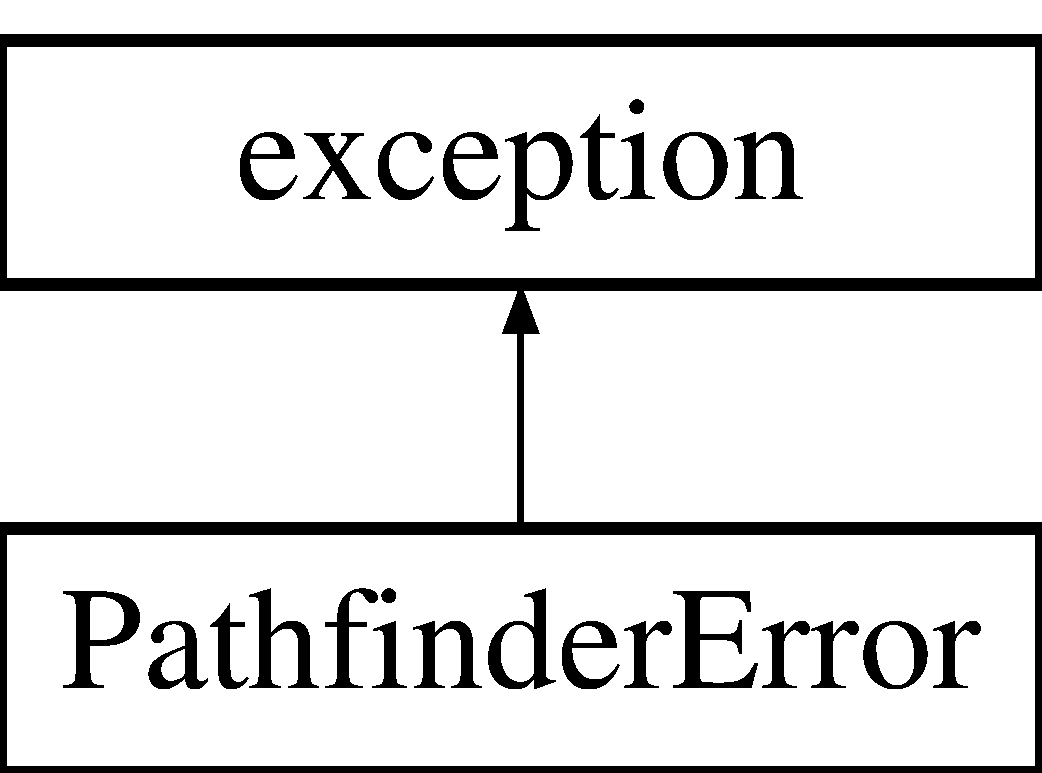
\includegraphics[height=2.000000cm]{class_pathfinder_error}
\end{center}
\end{figure}


The documentation for this class was generated from the following file\+:\begin{DoxyCompactItemize}
\item 
C\+:/\+Users/\+Alastair/\+Documents/\+Git\+Hub/comp250-\/\+A\+I-\/portfolio/\+Space\+Game/\+S\+D\+L\+\_\+project/Path\+Finder.\+h\end{DoxyCompactItemize}

\hypertarget{class_player_input}{}\section{Player\+Input Class Reference}
\label{class_player_input}\index{Player\+Input@{Player\+Input}}


The documentation for this class was generated from the following files\+:\begin{DoxyCompactItemize}
\item 
C\+:/\+Users/\+Alastair/\+Documents/\+Git\+Hub/comp250-\/\+A\+I-\/portfolio/\+Space\+Game/\+S\+D\+L\+\_\+project/Player\+Input.\+h\item 
C\+:/\+Users/\+Alastair/\+Documents/\+Git\+Hub/comp250-\/\+A\+I-\/portfolio/\+Space\+Game/\+S\+D\+L\+\_\+project/Player\+Input.\+cpp\end{DoxyCompactItemize}

\hypertarget{class_player_interaction}{}\section{Player\+Interaction Class Reference}
\label{class_player_interaction}\index{Player\+Interaction@{Player\+Interaction}}
\subsection*{Public Member Functions}
\begin{DoxyCompactItemize}
\item 
\mbox{\Hypertarget{class_player_interaction_a207b6d70549eee8a04669cafdd32b34b}\label{class_player_interaction_a207b6d70549eee8a04669cafdd32b34b}} 
void {\bfseries Interaction} (\hyperlink{class_level}{Level} \&grid, \hyperlink{class_agent}{Agent} \&agent)
\item 
\mbox{\Hypertarget{class_player_interaction_a9f3d8145f18c2dc0c1dcaae55ad02b02}\label{class_player_interaction_a9f3d8145f18c2dc0c1dcaae55ad02b02}} 
bool \hyperlink{class_player_interaction_a9f3d8145f18c2dc0c1dcaae55ad02b02}{get\+Door\+Status} ()
\begin{DoxyCompactList}\small\item\em Get door status. \end{DoxyCompactList}\item 
\mbox{\Hypertarget{class_player_interaction_a896e8a5f3c2312ac2050419ebd0704d9}\label{class_player_interaction_a896e8a5f3c2312ac2050419ebd0704d9}} 
bool \hyperlink{class_player_interaction_a896e8a5f3c2312ac2050419ebd0704d9}{set\+Door\+Status} (bool new\+Door\+Status)
\begin{DoxyCompactList}\small\item\em Set door status. \end{DoxyCompactList}\end{DoxyCompactItemize}


The documentation for this class was generated from the following files\+:\begin{DoxyCompactItemize}
\item 
C\+:/\+Users/\+Alastair/\+Documents/\+Git\+Hub/comp250-\/\+A\+I-\/portfolio/\+Space\+Game/\+S\+D\+L\+\_\+project/Agent\+Interaction.\+h\item 
C\+:/\+Users/\+Alastair/\+Documents/\+Git\+Hub/comp250-\/\+A\+I-\/portfolio/\+Space\+Game/\+S\+D\+L\+\_\+project/Agent\+Interaction.\+cpp\end{DoxyCompactItemize}

\hypertarget{class_player_stats}{}\section{Player\+Stats Class Reference}
\label{class_player_stats}\index{Player\+Stats@{Player\+Stats}}
Inheritance diagram for Player\+Stats\+:\begin{figure}[H]
\begin{center}
\leavevmode
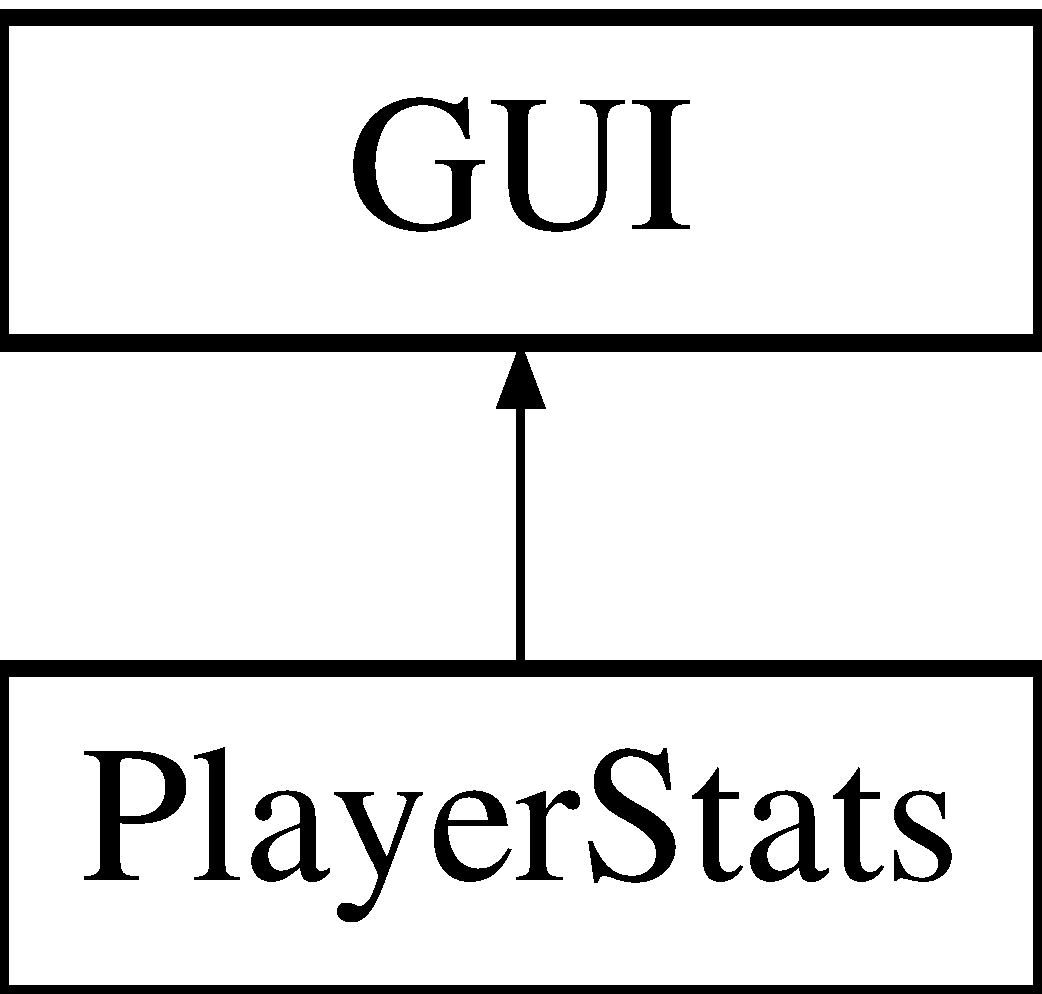
\includegraphics[height=2.000000cm]{class_player_stats}
\end{center}
\end{figure}
\subsection*{Public Member Functions}
\begin{DoxyCompactItemize}
\item 
\mbox{\Hypertarget{class_player_stats_afc6a36e074436e5b3ce922f9d192fb46}\label{class_player_stats_afc6a36e074436e5b3ce922f9d192fb46}} 
void {\bfseries render\+And\+Update\+Player\+Stats} (S\+D\+L\+\_\+\+Renderer $\ast$renderer, \hyperlink{class_agent_manager}{Agent\+Manager} \&character, int window\+Width, int window\+Height)
\end{DoxyCompactItemize}
\subsection*{Public Attributes}
\begin{DoxyCompactItemize}
\item 
\mbox{\Hypertarget{class_player_stats_acb028559ae1d74fbc8fda7eeac7c55ed}\label{class_player_stats_acb028559ae1d74fbc8fda7eeac7c55ed}} 
\hyperlink{class_texture}{Texture} {\bfseries player\+Stats\+Background\+Texture}
\item 
\mbox{\Hypertarget{class_player_stats_a6916703003f748e94c48a83bdb122654}\label{class_player_stats_a6916703003f748e94c48a83bdb122654}} 
\hyperlink{class_texture}{Texture} {\bfseries player\+Health}
\item 
\mbox{\Hypertarget{class_player_stats_a3fbd15fb06abec48e89d3e2e8538d245}\label{class_player_stats_a3fbd15fb06abec48e89d3e2e8538d245}} 
\hyperlink{class_texture}{Texture} {\bfseries player\+Oxygen}
\item 
\mbox{\Hypertarget{class_player_stats_a441c84f6a9b55e2bce22743e2da6cb49}\label{class_player_stats_a441c84f6a9b55e2bce22743e2da6cb49}} 
\hyperlink{class_texture}{Texture} {\bfseries player\+Hunger}
\item 
\mbox{\Hypertarget{class_player_stats_a7c81f7cdc2dd7afed2678b909f369389}\label{class_player_stats_a7c81f7cdc2dd7afed2678b909f369389}} 
\hyperlink{class_texture}{Texture} {\bfseries health\+Text}
\item 
\mbox{\Hypertarget{class_player_stats_a014ad313a6eb58fdd3d70f71fc5dc515}\label{class_player_stats_a014ad313a6eb58fdd3d70f71fc5dc515}} 
\hyperlink{class_texture}{Texture} {\bfseries oxygen\+Text}
\end{DoxyCompactItemize}
\subsection*{Protected Attributes}
\begin{DoxyCompactItemize}
\item 
\mbox{\Hypertarget{class_player_stats_a394ffdfa252f1b9e9b6b855dd5af1238}\label{class_player_stats_a394ffdfa252f1b9e9b6b855dd5af1238}} 
int {\bfseries bar\+X\+Pos}
\item 
\mbox{\Hypertarget{class_player_stats_a1d65749e6646e51ea8b398f33000d2ae}\label{class_player_stats_a1d65749e6646e51ea8b398f33000d2ae}} 
int {\bfseries bar\+Y\+Pos}
\item 
\mbox{\Hypertarget{class_player_stats_a0757964beff2e74c58cd4e073ab244e1}\label{class_player_stats_a0757964beff2e74c58cd4e073ab244e1}} 
int {\bfseries bar\+Height} = 20
\item 
\mbox{\Hypertarget{class_player_stats_aa996108ad33b0d0dcfa690836970d014}\label{class_player_stats_aa996108ad33b0d0dcfa690836970d014}} 
int {\bfseries bar\+Width} = 10
\end{DoxyCompactItemize}


The documentation for this class was generated from the following files\+:\begin{DoxyCompactItemize}
\item 
C\+:/\+Users/\+Alastair/\+Documents/\+Git\+Hub/comp250-\/\+A\+I-\/portfolio/\+Space\+Game/\+S\+D\+L\+\_\+project/Player\+Stats.\+h\item 
C\+:/\+Users/\+Alastair/\+Documents/\+Git\+Hub/comp250-\/\+A\+I-\/portfolio/\+Space\+Game/\+S\+D\+L\+\_\+project/Player\+Stats.\+cpp\end{DoxyCompactItemize}

\hypertarget{class_point}{}\section{Point Class Reference}
\label{class_point}\index{Point@{Point}}
\subsection*{Public Member Functions}
\begin{DoxyCompactItemize}
\item 
\mbox{\Hypertarget{class_point_a001c4958c310b248f5c26037aea38a9c}\label{class_point_a001c4958c310b248f5c26037aea38a9c}} 
{\bfseries Point} (int x, int y)
\item 
\mbox{\Hypertarget{class_point_ac9d5859db121c7d1b89ca89266dca0a3}\label{class_point_ac9d5859db121c7d1b89ca89266dca0a3}} 
int {\bfseries getX} () const
\item 
\mbox{\Hypertarget{class_point_a86d10ff46e08462c45b15a8c7ef62d61}\label{class_point_a86d10ff46e08462c45b15a8c7ef62d61}} 
int {\bfseries getY} () const
\end{DoxyCompactItemize}


The documentation for this class was generated from the following file\+:\begin{DoxyCompactItemize}
\item 
C\+:/\+Users/\+Alastair/\+Documents/\+Git\+Hub/comp250-\/\+A\+I-\/portfolio/\+Space\+Game/\+S\+D\+L\+\_\+project/Point.\+h\end{DoxyCompactItemize}

\hypertarget{class_render_cells}{}\section{Render\+Cells Class Reference}
\label{class_render_cells}\index{Render\+Cells@{Render\+Cells}}


The documentation for this class was generated from the following files\+:\begin{DoxyCompactItemize}
\item 
C\+:/\+Users/\+Alastair/\+Documents/\+Git\+Hub/comp250-\/\+A\+I-\/portfolio/\+Space\+Game/\+S\+D\+L\+\_\+project/Render\+Cells.\+h\item 
C\+:/\+Users/\+Alastair/\+Documents/\+Git\+Hub/comp250-\/\+A\+I-\/portfolio/\+Space\+Game/\+S\+D\+L\+\_\+project/Render\+Cells.\+cpp\end{DoxyCompactItemize}

\hypertarget{class_room_design}{}\section{Room\+Design Class Reference}
\label{class_room_design}\index{Room\+Design@{Room\+Design}}
\subsection*{Public Member Functions}
\begin{DoxyCompactItemize}
\item 
\mbox{\Hypertarget{class_room_design_a78f5ebaf5ec49ea9648a59e9b29738ac}\label{class_room_design_a78f5ebaf5ec49ea9648a59e9b29738ac}} 
void {\bfseries design\+Room} (\hyperlink{class_level}{Level} \&grid, int cellX, int cellY)
\item 
\mbox{\Hypertarget{class_room_design_a5f0cd01b980f0b624626c34e197c1de2}\label{class_room_design_a5f0cd01b980f0b624626c34e197c1de2}} 
bool {\bfseries check\+Center\+Cell} (\hyperlink{class_level}{Level} \&room, int cellX, int cellY)
\end{DoxyCompactItemize}


The documentation for this class was generated from the following files\+:\begin{DoxyCompactItemize}
\item 
C\+:/\+Users/\+Alastair/\+Documents/\+Git\+Hub/comp250-\/\+A\+I-\/portfolio/\+Space\+Game/\+S\+D\+L\+\_\+project/Room\+Design.\+h\item 
C\+:/\+Users/\+Alastair/\+Documents/\+Git\+Hub/comp250-\/\+A\+I-\/portfolio/\+Space\+Game/\+S\+D\+L\+\_\+project/Room\+Design.\+cpp\end{DoxyCompactItemize}

\hypertarget{class_behaviour_tree_1_1_root}{}\section{Behaviour\+Tree\+:\+:Root Class Reference}
\label{class_behaviour_tree_1_1_root}\index{Behaviour\+Tree\+::\+Root@{Behaviour\+Tree\+::\+Root}}
Inheritance diagram for Behaviour\+Tree\+:\+:Root\+:\begin{figure}[H]
\begin{center}
\leavevmode
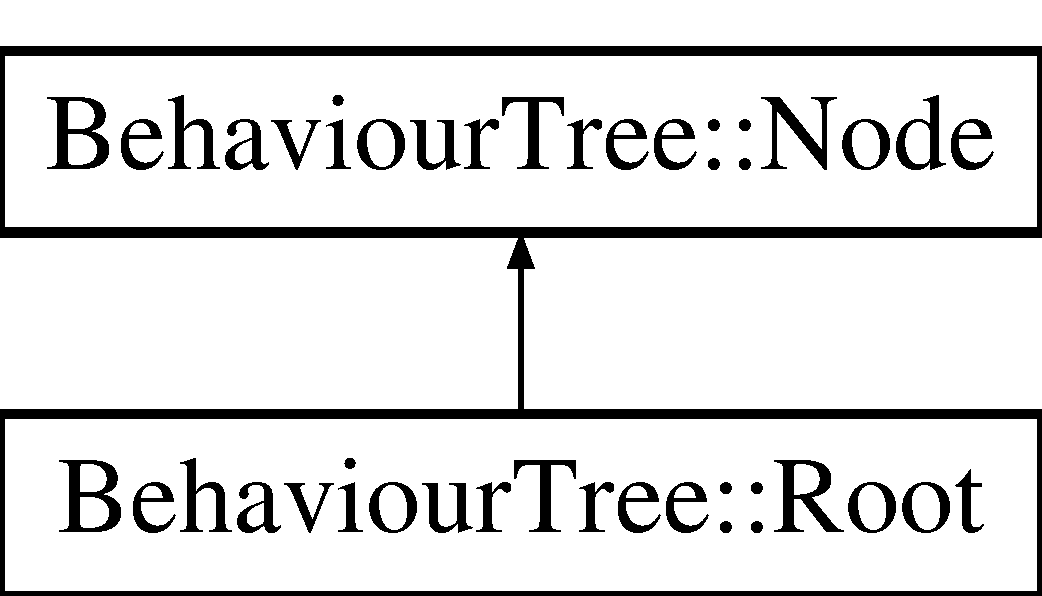
\includegraphics[height=2.000000cm]{class_behaviour_tree_1_1_root}
\end{center}
\end{figure}
\subsection*{Friends}
\begin{DoxyCompactItemize}
\item 
\mbox{\Hypertarget{class_behaviour_tree_1_1_root_ae563b66972c2eaf29474aa74fffa1d6f}\label{class_behaviour_tree_1_1_root_ae563b66972c2eaf29474aa74fffa1d6f}} 
class {\bfseries Behaviour\+Tree}
\end{DoxyCompactItemize}
\subsection*{Additional Inherited Members}


The documentation for this class was generated from the following file\+:\begin{DoxyCompactItemize}
\item 
C\+:/\+Users/\+Alastair/\+Documents/\+Git\+Hub/comp250-\/\+A\+I-\/portfolio/\+Space\+Game/\+S\+D\+L\+\_\+project/Behaviour\+Tree.\+h\end{DoxyCompactItemize}

\hypertarget{class_selector}{}\section{Selector Class Reference}
\label{class_selector}\index{Selector@{Selector}}
Inheritance diagram for Selector\+:\begin{figure}[H]
\begin{center}
\leavevmode
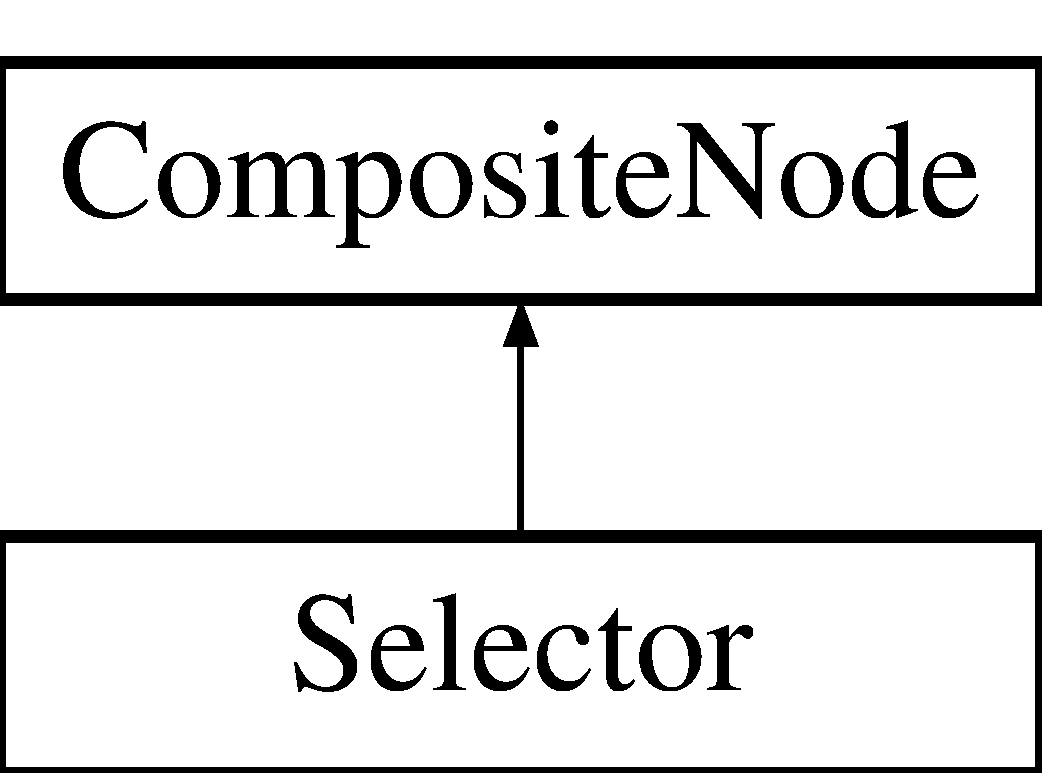
\includegraphics[height=2.000000cm]{class_selector}
\end{center}
\end{figure}
\subsection*{Public Member Functions}
\begin{DoxyCompactItemize}
\item 
\mbox{\Hypertarget{class_selector_a7bc8ca5615479b52488a392475411b20}\label{class_selector_a7bc8ca5615479b52488a392475411b20}} 
virtual bool {\bfseries run} () override
\end{DoxyCompactItemize}


The documentation for this class was generated from the following file\+:\begin{DoxyCompactItemize}
\item 
C\+:/\+Users/\+Alastair/\+Documents/\+Git\+Hub/comp250-\/\+A\+I-\/portfolio/\+Space\+Game/\+S\+D\+L\+\_\+project/Selector.\+h\end{DoxyCompactItemize}

\hypertarget{class_behaviour_tree_1_1_selector}{}\section{Behaviour\+Tree\+:\+:Selector Class Reference}
\label{class_behaviour_tree_1_1_selector}\index{Behaviour\+Tree\+::\+Selector@{Behaviour\+Tree\+::\+Selector}}
Inheritance diagram for Behaviour\+Tree\+:\+:Selector\+:\begin{figure}[H]
\begin{center}
\leavevmode
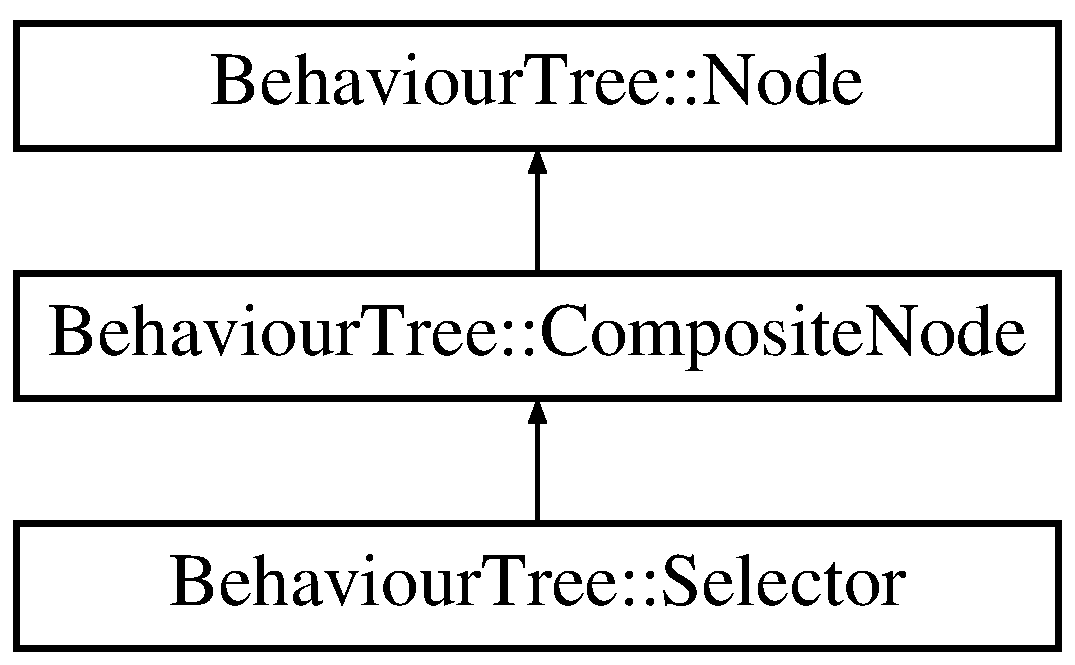
\includegraphics[height=3.000000cm]{class_behaviour_tree_1_1_selector}
\end{center}
\end{figure}
\subsection*{Public Member Functions}
\begin{DoxyCompactItemize}
\item 
\mbox{\Hypertarget{class_behaviour_tree_1_1_selector_ada6391d7dff66c89fb7da135bbcb2f4f}\label{class_behaviour_tree_1_1_selector_ada6391d7dff66c89fb7da135bbcb2f4f}} 
virtual bool {\bfseries run} () override
\end{DoxyCompactItemize}
\subsection*{Additional Inherited Members}


The documentation for this class was generated from the following file\+:\begin{DoxyCompactItemize}
\item 
C\+:/\+Users/\+Alastair/\+Documents/\+Git\+Hub/comp250-\/\+A\+I-\/portfolio/\+Space\+Game/\+S\+D\+L\+\_\+project/Behaviour\+Tree.\+h\end{DoxyCompactItemize}

\hypertarget{class_behaviour_tree_1_1_sequence}{}\section{Behaviour\+Tree\+:\+:Sequence Class Reference}
\label{class_behaviour_tree_1_1_sequence}\index{Behaviour\+Tree\+::\+Sequence@{Behaviour\+Tree\+::\+Sequence}}
Inheritance diagram for Behaviour\+Tree\+:\+:Sequence\+:\begin{figure}[H]
\begin{center}
\leavevmode
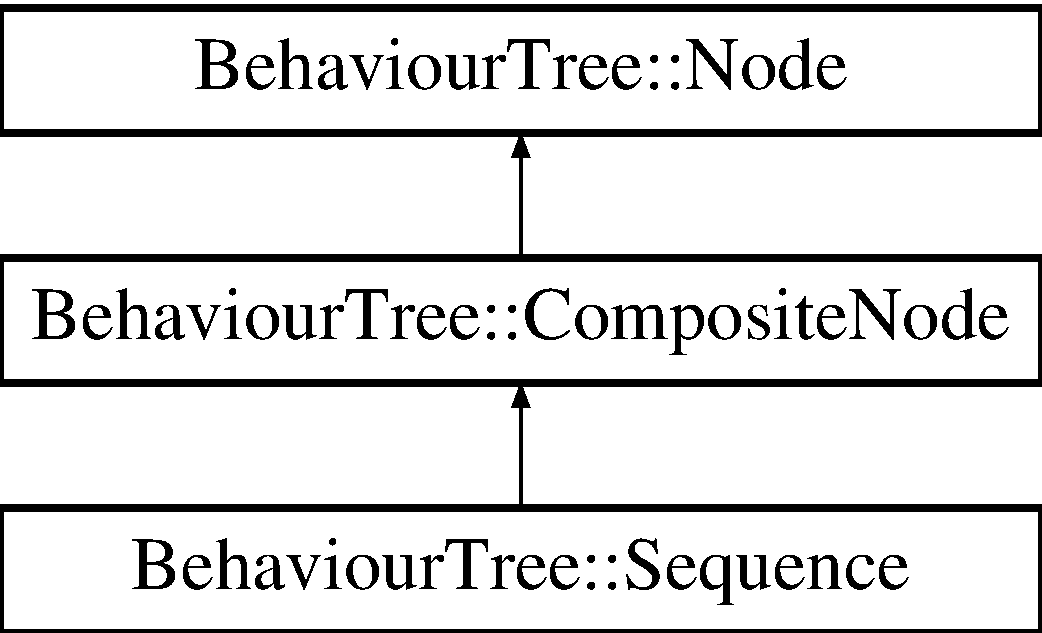
\includegraphics[height=3.000000cm]{class_behaviour_tree_1_1_sequence}
\end{center}
\end{figure}
\subsection*{Public Member Functions}
\begin{DoxyCompactItemize}
\item 
\mbox{\Hypertarget{class_behaviour_tree_1_1_sequence_a041ffcaef411be79a5aaade6e7b1c7b1}\label{class_behaviour_tree_1_1_sequence_a041ffcaef411be79a5aaade6e7b1c7b1}} 
virtual bool {\bfseries run} () override
\end{DoxyCompactItemize}
\subsection*{Additional Inherited Members}


The documentation for this class was generated from the following file\+:\begin{DoxyCompactItemize}
\item 
C\+:/\+Users/\+Alastair/\+Documents/\+Git\+Hub/comp250-\/\+A\+I-\/portfolio/\+Space\+Game/\+S\+D\+L\+\_\+project/Behaviour\+Tree.\+h\end{DoxyCompactItemize}

\hypertarget{class_sequence}{}\section{Sequence Class Reference}
\label{class_sequence}\index{Sequence@{Sequence}}
Inheritance diagram for Sequence\+:\begin{figure}[H]
\begin{center}
\leavevmode
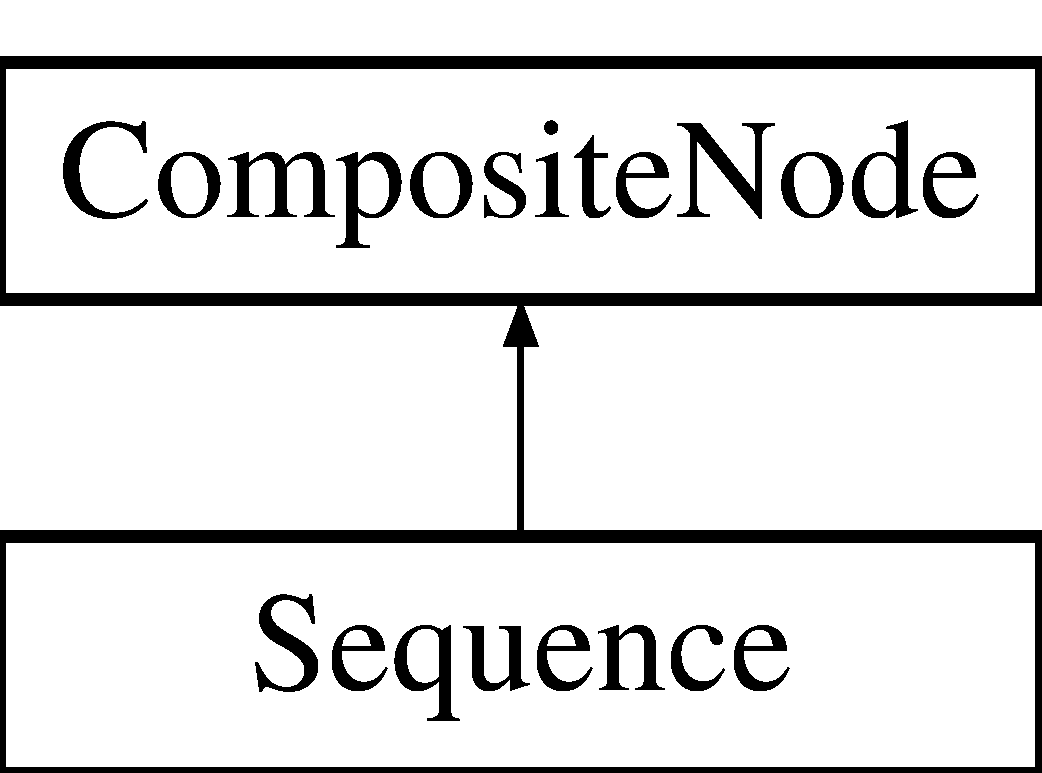
\includegraphics[height=2.000000cm]{class_sequence}
\end{center}
\end{figure}
\subsection*{Public Member Functions}
\begin{DoxyCompactItemize}
\item 
\mbox{\Hypertarget{class_sequence_ad9eb21db650776a278d3f2c1e7499dd8}\label{class_sequence_ad9eb21db650776a278d3f2c1e7499dd8}} 
virtual bool {\bfseries run} () override
\end{DoxyCompactItemize}


The documentation for this class was generated from the following file\+:\begin{DoxyCompactItemize}
\item 
C\+:/\+Users/\+Alastair/\+Documents/\+Git\+Hub/comp250-\/\+A\+I-\/portfolio/\+Space\+Game/\+S\+D\+L\+\_\+project/Sequence.\+h\end{DoxyCompactItemize}

\hypertarget{class_ship}{}\section{Ship Class Reference}
\label{class_ship}\index{Ship@{Ship}}
Inheritance diagram for Ship\+:\begin{figure}[H]
\begin{center}
\leavevmode
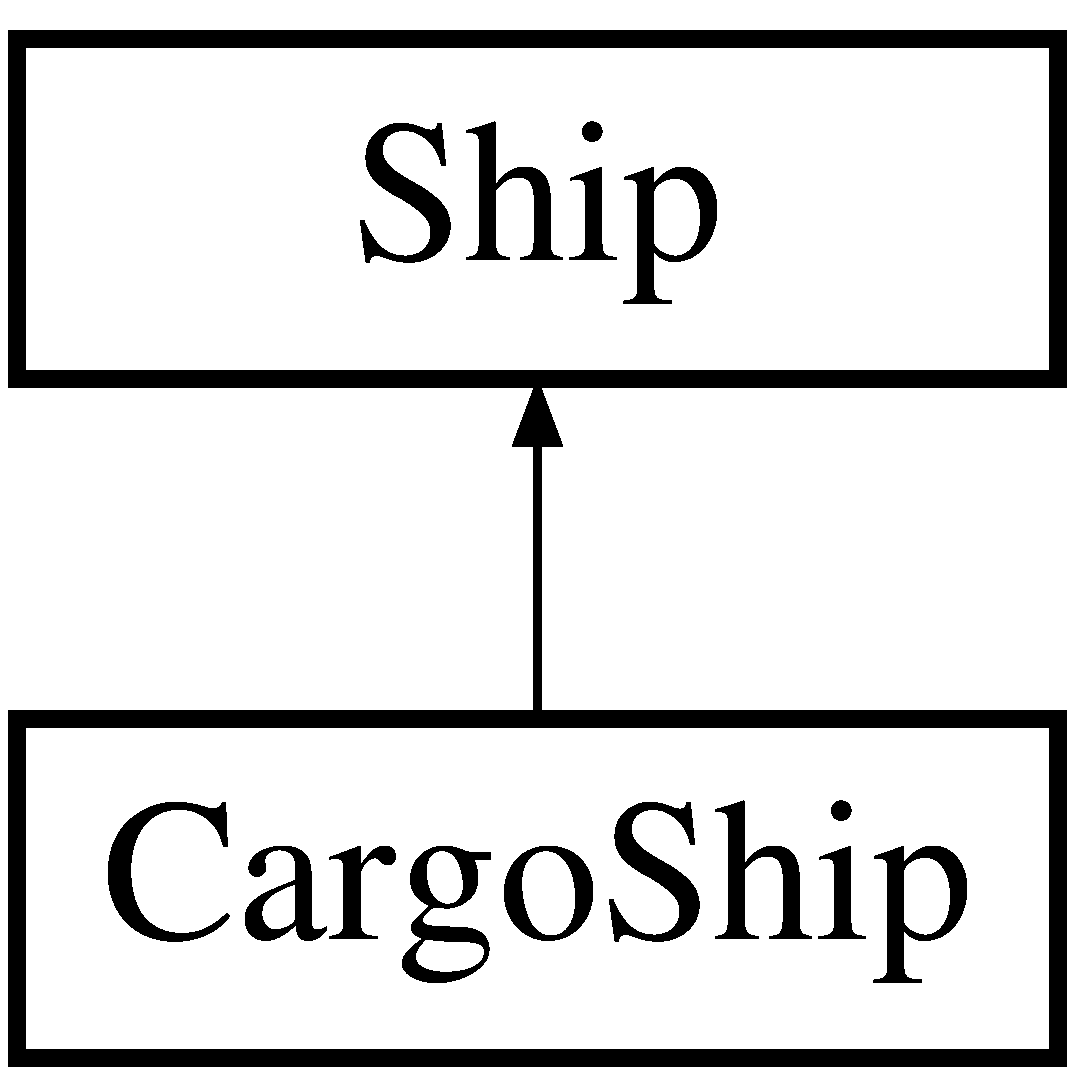
\includegraphics[height=2.000000cm]{class_ship}
\end{center}
\end{figure}
\subsection*{Public Member Functions}
\begin{DoxyCompactItemize}
\item 
\mbox{\Hypertarget{class_ship_ab7608fcfc4d27c678aacaf9bfd68a462}\label{class_ship_ab7608fcfc4d27c678aacaf9bfd68a462}} 
\hyperlink{class_ship_ab7608fcfc4d27c678aacaf9bfd68a462}{Ship} ()
\begin{DoxyCompactList}\small\item\em Constructor. \end{DoxyCompactList}\item 
\mbox{\Hypertarget{class_ship_a43cd6eeaffc11b49239b091621963a65}\label{class_ship_a43cd6eeaffc11b49239b091621963a65}} 
\hyperlink{class_ship_a43cd6eeaffc11b49239b091621963a65}{$\sim$\+Ship} ()
\begin{DoxyCompactList}\small\item\em Destructor. \end{DoxyCompactList}\item 
\mbox{\Hypertarget{class_ship_a846040dad9c03dec8d6bdfc24753f05b}\label{class_ship_a846040dad9c03dec8d6bdfc24753f05b}} 
int \hyperlink{class_ship_a846040dad9c03dec8d6bdfc24753f05b}{getX} ()
\begin{DoxyCompactList}\small\item\em Get X position. \end{DoxyCompactList}\item 
\mbox{\Hypertarget{class_ship_a0cde4e9b74fb71cbf61f79e0a1b74059}\label{class_ship_a0cde4e9b74fb71cbf61f79e0a1b74059}} 
int \hyperlink{class_ship_a0cde4e9b74fb71cbf61f79e0a1b74059}{getY} ()
\begin{DoxyCompactList}\small\item\em Get Y position. \end{DoxyCompactList}\item 
\mbox{\Hypertarget{class_ship_a62498f72ced4db442cc5c8eb288aa8ad}\label{class_ship_a62498f72ced4db442cc5c8eb288aa8ad}} 
int \hyperlink{class_ship_a62498f72ced4db442cc5c8eb288aa8ad}{setX} (int newX)
\begin{DoxyCompactList}\small\item\em Set X position. \end{DoxyCompactList}\item 
\mbox{\Hypertarget{class_ship_ac751c2fde09e5e92dc53f8bf29711cb0}\label{class_ship_ac751c2fde09e5e92dc53f8bf29711cb0}} 
int \hyperlink{class_ship_ac751c2fde09e5e92dc53f8bf29711cb0}{setY} (int newY)
\begin{DoxyCompactList}\small\item\em Set Y position. \end{DoxyCompactList}\item 
\mbox{\Hypertarget{class_ship_aeba3adb876e7c83760448245f6950d8b}\label{class_ship_aeba3adb876e7c83760448245f6950d8b}} 
int \hyperlink{class_ship_aeba3adb876e7c83760448245f6950d8b}{get\+Width} ()
\begin{DoxyCompactList}\small\item\em Get width. \end{DoxyCompactList}\item 
\mbox{\Hypertarget{class_ship_aa776da1fa8f5fd12019ec0030ae138c0}\label{class_ship_aa776da1fa8f5fd12019ec0030ae138c0}} 
int \hyperlink{class_ship_aa776da1fa8f5fd12019ec0030ae138c0}{get\+Height} ()
\begin{DoxyCompactList}\small\item\em Get Hight. \end{DoxyCompactList}\item 
\mbox{\Hypertarget{class_ship_ab9524ec89dd6cd0e25974b36143cf86a}\label{class_ship_ab9524ec89dd6cd0e25974b36143cf86a}} 
int {\bfseries set\+Width} (int new\+Width)
\item 
\mbox{\Hypertarget{class_ship_a20709bf79b466043ccb120c20af894b1}\label{class_ship_a20709bf79b466043ccb120c20af894b1}} 
int {\bfseries set\+Height} (int new\+Height)
\item 
\mbox{\Hypertarget{class_ship_af91376e255cbd3d1654b9759821f4a06}\label{class_ship_af91376e255cbd3d1654b9759821f4a06}} 
std\+::string \hyperlink{class_ship_af91376e255cbd3d1654b9759821f4a06}{get\+Ship\+Status} ()
\begin{DoxyCompactList}\small\item\em Get and Set ship status. \end{DoxyCompactList}\item 
\mbox{\Hypertarget{class_ship_a733169da5bc3c07603f1ea35c0bb5889}\label{class_ship_a733169da5bc3c07603f1ea35c0bb5889}} 
std\+::string {\bfseries set\+Ship\+Status} (std\+::string new\+Ship\+Status)
\item 
\mbox{\Hypertarget{class_ship_a639f56a1c08568f30a15e26a767fe855}\label{class_ship_a639f56a1c08568f30a15e26a767fe855}} 
int \hyperlink{class_ship_a639f56a1c08568f30a15e26a767fe855}{get\+Amount\+Of\+Cargo} ()
\begin{DoxyCompactList}\small\item\em Get the ships cargo. \end{DoxyCompactList}\item 
\mbox{\Hypertarget{class_ship_aabc3adc1bd83da7022bbfb8e5bc06757}\label{class_ship_aabc3adc1bd83da7022bbfb8e5bc06757}} 
int \hyperlink{class_ship_aabc3adc1bd83da7022bbfb8e5bc06757}{set\+Amount\+Of\+Cargo} (int New\+Amount\+Of\+Cargo)
\begin{DoxyCompactList}\small\item\em Set the ships cargo. \end{DoxyCompactList}\item 
\mbox{\Hypertarget{class_ship_a3ed6ad81c7733204557276a176cb8621}\label{class_ship_a3ed6ad81c7733204557276a176cb8621}} 
void {\bfseries Render\+Ship} (S\+D\+L\+\_\+\+Renderer $\ast$renderer, \hyperlink{class_ship}{Ship} \&ship)
\end{DoxyCompactItemize}
\subsection*{Public Attributes}
\begin{DoxyCompactItemize}
\item 
\mbox{\Hypertarget{class_ship_a37c2a087a444a12e1fe7917251fd7f26}\label{class_ship_a37c2a087a444a12e1fe7917251fd7f26}} 
bool \hyperlink{class_ship_a37c2a087a444a12e1fe7917251fd7f26}{ship\+Placed\+On\+Docking\+Path} = false
\begin{DoxyCompactList}\small\item\em If the ship has be placed on the path to the dock. \end{DoxyCompactList}\item 
\mbox{\Hypertarget{class_ship_a9df053208d5a04dbe31186ad7e6008bd}\label{class_ship_a9df053208d5a04dbe31186ad7e6008bd}} 
bool \hyperlink{class_ship_a9df053208d5a04dbe31186ad7e6008bd}{is\+Docked} = false
\begin{DoxyCompactList}\small\item\em If the ship is docked. \end{DoxyCompactList}\item 
\mbox{\Hypertarget{class_ship_a8c6c6302e1a88d4902176ee6c6a7a4e2}\label{class_ship_a8c6c6302e1a88d4902176ee6c6a7a4e2}} 
\hyperlink{class_texture}{Texture} \hyperlink{class_ship_a8c6c6302e1a88d4902176ee6c6a7a4e2}{Cargo\+Ship\+Texture}
\begin{DoxyCompactList}\small\item\em Is the texture for the cargo ship. \end{DoxyCompactList}\end{DoxyCompactItemize}


The documentation for this class was generated from the following files\+:\begin{DoxyCompactItemize}
\item 
C\+:/\+Users/\+Alastair/\+Documents/\+Git\+Hub/comp250-\/\+A\+I-\/portfolio/\+Space\+Game/\+S\+D\+L\+\_\+project/Ship.\+h\item 
C\+:/\+Users/\+Alastair/\+Documents/\+Git\+Hub/comp250-\/\+A\+I-\/portfolio/\+Space\+Game/\+S\+D\+L\+\_\+project/Ship.\+cpp\end{DoxyCompactItemize}

\hypertarget{class_ship_manager}{}\section{Ship\+Manager Class Reference}
\label{class_ship_manager}\index{Ship\+Manager@{Ship\+Manager}}
\subsection*{Public Member Functions}
\begin{DoxyCompactItemize}
\item 
\mbox{\Hypertarget{class_ship_manager_a5c7bc1182e2083180ec4e9f561880ba6}\label{class_ship_manager_a5c7bc1182e2083180ec4e9f561880ba6}} 
\hyperlink{class_ship_manager_a5c7bc1182e2083180ec4e9f561880ba6}{Ship\+Manager} ()
\begin{DoxyCompactList}\small\item\em Constructor. \end{DoxyCompactList}\item 
\mbox{\Hypertarget{class_ship_manager_a12f43d1ff5f1d3657030c18be90745bc}\label{class_ship_manager_a12f43d1ff5f1d3657030c18be90745bc}} 
\hyperlink{class_ship_manager_a12f43d1ff5f1d3657030c18be90745bc}{$\sim$\+Ship\+Manager} ()
\begin{DoxyCompactList}\small\item\em Destructor. \end{DoxyCompactList}\item 
\mbox{\Hypertarget{class_ship_manager_adb8e868a32060cef24240c7b9699ba20}\label{class_ship_manager_adb8e868a32060cef24240c7b9699ba20}} 
void \hyperlink{class_ship_manager_adb8e868a32060cef24240c7b9699ba20}{move\+Ship\+To\+Dock} (\hyperlink{class_level}{Level} \&level, \hyperlink{class_ship}{Ship} \&ship, int direction)
\begin{DoxyCompactList}\small\item\em Spawns a ship and moves it to the dock. \end{DoxyCompactList}\item 
\mbox{\Hypertarget{class_ship_manager_a24db308b29f58e4de824164047596cd0}\label{class_ship_manager_a24db308b29f58e4de824164047596cd0}} 
void {\bfseries ship\+Timer} (\hyperlink{class_level}{Level} \&level, std\+::vector$<$ \hyperlink{class_ship}{Ship} $>$ \&all\+Ships)
\item 
\mbox{\Hypertarget{class_ship_manager_a1350a0d3b9dc013e6e7839cb5e3d17e9}\label{class_ship_manager_a1350a0d3b9dc013e6e7839cb5e3d17e9}} 
void {\bfseries find\+Ship\+Spawn} (\hyperlink{class_level}{Level} \&level, \hyperlink{class_ship}{Ship} \&ship)
\item 
\mbox{\Hypertarget{class_ship_manager_a2a48ef5e8de1d665890fce631b652738}\label{class_ship_manager_a2a48ef5e8de1d665890fce631b652738}} 
void {\bfseries create\+Ship} (std\+::vector$<$ \hyperlink{class_ship}{Ship} $>$ \&all\+Ships)
\item 
\mbox{\Hypertarget{class_ship_manager_a4592885107ee1ebf4b67e09c21e0cd19}\label{class_ship_manager_a4592885107ee1ebf4b67e09c21e0cd19}} 
void {\bfseries render\+Ship} (std\+::vector$<$ \hyperlink{class_ship}{Ship} $>$ \&allships, S\+D\+L\+\_\+\+Renderer $\ast$renderer)
\item 
\mbox{\Hypertarget{class_ship_manager_a6153e9fc458598fde00bde88f8e4a97f}\label{class_ship_manager_a6153e9fc458598fde00bde88f8e4a97f}} 
void {\bfseries ship\+Docked} (\hyperlink{class_level}{Level} \&level, \hyperlink{class_ship}{Ship} \&ship)
\end{DoxyCompactItemize}
\subsection*{Public Attributes}
\begin{DoxyCompactItemize}
\item 
\mbox{\Hypertarget{class_ship_manager_a95b1e086a0869f8710eb08f34361a265}\label{class_ship_manager_a95b1e086a0869f8710eb08f34361a265}} 
bool {\bfseries ship\+Already\+Spawned} = false
\item 
\mbox{\Hypertarget{class_ship_manager_a94034b450484f60571f2a5adbe598367}\label{class_ship_manager_a94034b450484f60571f2a5adbe598367}} 
bool {\bfseries there\+Is\+Docking\+Path} = false
\item 
\mbox{\Hypertarget{class_ship_manager_a28167f646696e508c96ee8272bbfbc12}\label{class_ship_manager_a28167f646696e508c96ee8272bbfbc12}} 
bool {\bfseries fill\+Level\+With\+Cells} = true
\end{DoxyCompactItemize}


The documentation for this class was generated from the following files\+:\begin{DoxyCompactItemize}
\item 
C\+:/\+Users/\+Alastair/\+Documents/\+Git\+Hub/comp250-\/\+A\+I-\/portfolio/\+Space\+Game/\+S\+D\+L\+\_\+project/Ship\+Manager.\+h\item 
C\+:/\+Users/\+Alastair/\+Documents/\+Git\+Hub/comp250-\/\+A\+I-\/portfolio/\+Space\+Game/\+S\+D\+L\+\_\+project/Ship\+Manager.\+cpp\end{DoxyCompactItemize}

\hypertarget{class_space_game}{}\section{Space\+Game Class Reference}
\label{class_space_game}\index{Space\+Game@{Space\+Game}}


The main class.  




{\ttfamily \#include $<$Space\+Game.\+h$>$}

\subsection*{Public Member Functions}
\begin{DoxyCompactItemize}
\item 
\mbox{\Hypertarget{class_space_game_a36f837658700f0b32d5b0935231bf721}\label{class_space_game_a36f837658700f0b32d5b0935231bf721}} 
\hyperlink{class_space_game_a36f837658700f0b32d5b0935231bf721}{Space\+Game} ()
\begin{DoxyCompactList}\small\item\em A constructor. \end{DoxyCompactList}\item 
\mbox{\Hypertarget{class_space_game_ad166a3a331825b32a484375b80fc17b5}\label{class_space_game_ad166a3a331825b32a484375b80fc17b5}} 
\hyperlink{class_space_game_ad166a3a331825b32a484375b80fc17b5}{$\sim$\+Space\+Game} ()
\begin{DoxyCompactList}\small\item\em A deconstructor. \end{DoxyCompactList}\item 
\mbox{\Hypertarget{class_space_game_ab266e118927854120d3185722c9e448d}\label{class_space_game_ab266e118927854120d3185722c9e448d}} 
void \hyperlink{class_space_game_ab266e118927854120d3185722c9e448d}{run} ()
\begin{DoxyCompactList}\small\item\em Main Run loop. \end{DoxyCompactList}\item 
\mbox{\Hypertarget{class_space_game_a5cb4e8dfad6d5080c5d1cec959e40767}\label{class_space_game_a5cb4e8dfad6d5080c5d1cec959e40767}} 
void \hyperlink{class_space_game_a5cb4e8dfad6d5080c5d1cec959e40767}{delete\+Vectors} ()
\begin{DoxyCompactList}\small\item\em Removes all the data from stored vectors. \end{DoxyCompactList}\end{DoxyCompactItemize}
\subsection*{Public Attributes}
\begin{DoxyCompactItemize}
\item 
\mbox{\Hypertarget{class_space_game_a13b9266a848dbbd36811fcd958c14e72}\label{class_space_game_a13b9266a848dbbd36811fcd958c14e72}} 
\hyperlink{class_level}{Level} \hyperlink{class_space_game_a13b9266a848dbbd36811fcd958c14e72}{level}
\begin{DoxyCompactList}\small\item\em Initalising all classes needed for game. \end{DoxyCompactList}\item 
\mbox{\Hypertarget{class_space_game_abb8dbac6e9bf0c31d618be71dec942f5}\label{class_space_game_abb8dbac6e9bf0c31d618be71dec942f5}} 
\hyperlink{class_game_settings}{Game\+Settings} {\bfseries game\+Settings}
\item 
\mbox{\Hypertarget{class_space_game_ad10824caf8335c970fc6031ead3a63a8}\label{class_space_game_ad10824caf8335c970fc6031ead3a63a8}} 
\hyperlink{class_map}{Map} {\bfseries map\+Loader}
\item 
\mbox{\Hypertarget{class_space_game_a33e95e1290f822fe6568da5b8493f186}\label{class_space_game_a33e95e1290f822fe6568da5b8493f186}} 
\hyperlink{class_room_design}{Room\+Design} {\bfseries designroom}
\item 
\mbox{\Hypertarget{class_space_game_a97f7eec404779c9a0ac068ee22afec93}\label{class_space_game_a97f7eec404779c9a0ac068ee22afec93}} 
\hyperlink{class_oxygen}{Oxygen} {\bfseries oxygen}
\item 
\mbox{\Hypertarget{class_space_game_ac42eea67a31352b71500da32875b66b9}\label{class_space_game_ac42eea67a31352b71500da32875b66b9}} 
\hyperlink{class_fire}{Fire} {\bfseries fire}
\item 
\mbox{\Hypertarget{class_space_game_ab726e64a5e0e2a1847473d8e8528a1c8}\label{class_space_game_ab726e64a5e0e2a1847473d8e8528a1c8}} 
\hyperlink{class_player_interaction}{Player\+Interaction} {\bfseries character\+Interaction}
\item 
\mbox{\Hypertarget{class_space_game_a23ccc84ea819eeb2d2eab875fd8a4fe8}\label{class_space_game_a23ccc84ea819eeb2d2eab875fd8a4fe8}} 
\hyperlink{class_agent_manager}{Agent\+Manager} {\bfseries agent\+Manager}
\item 
\mbox{\Hypertarget{class_space_game_ac09355a77f5c400853bbcd5a197f1048}\label{class_space_game_ac09355a77f5c400853bbcd5a197f1048}} 
\hyperlink{class_cell}{Cell} {\bfseries cell}
\item 
\mbox{\Hypertarget{class_space_game_afb53554bed850fa764f75a50cc8cb2d4}\label{class_space_game_afb53554bed850fa764f75a50cc8cb2d4}} 
\hyperlink{class_tool_bar}{Tool\+Bar} {\bfseries toolbar}
\item 
\mbox{\Hypertarget{class_space_game_ab64693c91c01491cb2de38ae66ca73a2}\label{class_space_game_ab64693c91c01491cb2de38ae66ca73a2}} 
\hyperlink{class_escape_menu}{Escape\+Menu} {\bfseries escapemenu}
\item 
\mbox{\Hypertarget{class_space_game_a6e1f6ecc91ec7f3e4d66af8dcf6d5b5d}\label{class_space_game_a6e1f6ecc91ec7f3e4d66af8dcf6d5b5d}} 
\hyperlink{class_docking_doors}{Docking\+Doors} {\bfseries dockingdoors}
\item 
\mbox{\Hypertarget{class_space_game_ad778e0b9cab95f330549ae520ee7d789}\label{class_space_game_ad778e0b9cab95f330549ae520ee7d789}} 
\hyperlink{class_ship_manager}{Ship\+Manager} {\bfseries shipmanager}
\item 
\mbox{\Hypertarget{class_space_game_a4e057dd0dc2a70ed37a438ff10a8a294}\label{class_space_game_a4e057dd0dc2a70ed37a438ff10a8a294}} 
\hyperlink{class_player_stats}{Player\+Stats} {\bfseries playerstats}
\item 
\mbox{\Hypertarget{class_space_game_a39c6c796116b3865a11ff6174c0a6650}\label{class_space_game_a39c6c796116b3865a11ff6174c0a6650}} 
\hyperlink{class_cell_rendering}{Cell\+Rendering} {\bfseries cellrenderer}
\item 
\mbox{\Hypertarget{class_space_game_a06039d5815d6a3110dc7eb38a542d25e}\label{class_space_game_a06039d5815d6a3110dc7eb38a542d25e}} 
\hyperlink{class_hydroponics}{Hydroponics} {\bfseries hydroponics}
\item 
std\+::vector$<$ \hyperlink{class_hydroponics}{Hydroponics} $>$ \hyperlink{class_space_game_a59e762b653e6952d65f8dd51b055bc2f}{all\+Hydroponics\+Farms}
\begin{DoxyCompactList}\small\item\em Conains the list of nodes that makes the path. \end{DoxyCompactList}\item 
\mbox{\Hypertarget{class_space_game_a3ec694d86ca1d451bb3ab246785c5988}\label{class_space_game_a3ec694d86ca1d451bb3ab246785c5988}} 
std\+::vector$<$ \hyperlink{class_ship}{Ship} $>$ \hyperlink{class_space_game_a3ec694d86ca1d451bb3ab246785c5988}{all\+Ships}
\begin{DoxyCompactList}\small\item\em Contains a list of all the ship. \end{DoxyCompactList}\item 
\mbox{\Hypertarget{class_space_game_a969661713225da053f9c046f7ce2415b}\label{class_space_game_a969661713225da053f9c046f7ce2415b}} 
bool {\bfseries fill\+Level\+With\+Cells} = false
\item 
\mbox{\Hypertarget{class_space_game_ac1ec1fbe39ce5b122675a7fd668c8ea3}\label{class_space_game_ac1ec1fbe39ce5b122675a7fd668c8ea3}} 
int \hyperlink{class_space_game_ac1ec1fbe39ce5b122675a7fd668c8ea3}{W\+I\+N\+D\+O\+W\+\_\+\+W\+I\+D\+TH} = game\+Settings.\+W\+I\+N\+D\+O\+W\+\_\+\+W\+I\+D\+TH
\begin{DoxyCompactList}\small\item\em The window width. \end{DoxyCompactList}\item 
\mbox{\Hypertarget{class_space_game_aa557f0135ff2281fbfe7eaa69723b6c5}\label{class_space_game_aa557f0135ff2281fbfe7eaa69723b6c5}} 
int \hyperlink{class_space_game_aa557f0135ff2281fbfe7eaa69723b6c5}{W\+I\+N\+D\+O\+W\+\_\+\+H\+E\+I\+G\+HT} = game\+Settings.\+W\+I\+N\+D\+O\+W\+\_\+\+H\+E\+I\+G\+HT
\begin{DoxyCompactList}\small\item\em The window height. \end{DoxyCompactList}\item 
\mbox{\Hypertarget{class_space_game_a23e048b8ccf23343a4f9a9f67d1df3ba}\label{class_space_game_a23e048b8ccf23343a4f9a9f67d1df3ba}} 
int \hyperlink{class_space_game_a23e048b8ccf23343a4f9a9f67d1df3ba}{mouse\+\_\+X}
\begin{DoxyCompactList}\small\item\em Coordinates of the mouse. \end{DoxyCompactList}\item 
\mbox{\Hypertarget{class_space_game_a503f8ad7c3466ce91ab40f74b29b0097}\label{class_space_game_a503f8ad7c3466ce91ab40f74b29b0097}} 
int {\bfseries mouse\+\_\+Y}
\end{DoxyCompactItemize}


\subsection{Detailed Description}
The main class. 

This is the main class where the game is laoded and run. 

\subsection{Member Data Documentation}
\mbox{\Hypertarget{class_space_game_a59e762b653e6952d65f8dd51b055bc2f}\label{class_space_game_a59e762b653e6952d65f8dd51b055bc2f}} 
\index{Space\+Game@{Space\+Game}!all\+Hydroponics\+Farms@{all\+Hydroponics\+Farms}}
\index{all\+Hydroponics\+Farms@{all\+Hydroponics\+Farms}!Space\+Game@{Space\+Game}}
\subsubsection{\texorpdfstring{all\+Hydroponics\+Farms}{allHydroponicsFarms}}
{\footnotesize\ttfamily std\+::vector$<$\hyperlink{class_hydroponics}{Hydroponics}$>$ Space\+Game\+::all\+Hydroponics\+Farms}



Conains the list of nodes that makes the path. 

Contains a list of all the hydroponic farms 

The documentation for this class was generated from the following files\+:\begin{DoxyCompactItemize}
\item 
C\+:/\+Users/\+Alastair/\+Documents/\+Git\+Hub/comp250-\/\+A\+I-\/portfolio/\+Space\+Game/\+S\+D\+L\+\_\+project/Space\+Game.\+h\item 
C\+:/\+Users/\+Alastair/\+Documents/\+Git\+Hub/comp250-\/\+A\+I-\/portfolio/\+Space\+Game/\+S\+D\+L\+\_\+project/Space\+Game.\+cpp\end{DoxyCompactItemize}

\hypertarget{class_texture}{}\section{Texture Class Reference}
\label{class_texture}\index{Texture@{Texture}}


Loads and renders images in the window.  




{\ttfamily \#include $<$Texture.\+h$>$}

\subsection*{Public Member Functions}
\begin{DoxyCompactItemize}
\item 
\hyperlink{class_texture_ab303a4548e5c5822de490b99b5d3f928}{Texture} (const std\+::string \&file\+Name)
\begin{DoxyCompactList}\small\item\em A constructor. \end{DoxyCompactList}\item 
\mbox{\Hypertarget{class_texture_a09c4bcb7462f64c1d20fa69dba3cee8a}\label{class_texture_a09c4bcb7462f64c1d20fa69dba3cee8a}} 
\hyperlink{class_texture_a09c4bcb7462f64c1d20fa69dba3cee8a}{$\sim$\+Texture} ()
\begin{DoxyCompactList}\small\item\em A destructor. \end{DoxyCompactList}\item 
\mbox{\Hypertarget{class_texture_a684e829a07a77e13b17a10e65734562b}\label{class_texture_a684e829a07a77e13b17a10e65734562b}} 
S\+D\+L\+\_\+\+Texture $\ast$ \hyperlink{class_texture_a684e829a07a77e13b17a10e65734562b}{get\+Texture} ()
\begin{DoxyCompactList}\small\item\em Loads the texture. \end{DoxyCompactList}\item 
\mbox{\Hypertarget{class_texture_a3a541d62f7e282d8f206a0b6a4022006}\label{class_texture_a3a541d62f7e282d8f206a0b6a4022006}} 
void \hyperlink{class_texture_a3a541d62f7e282d8f206a0b6a4022006}{render} (S\+D\+L\+\_\+\+Renderer $\ast$renderer, int x, int y, int width, int height)
\begin{DoxyCompactList}\small\item\em Renders the image in the window. \end{DoxyCompactList}\item 
\mbox{\Hypertarget{class_texture_abadbea608d1cbfb2663e0f72f931ac47}\label{class_texture_abadbea608d1cbfb2663e0f72f931ac47}} 
void \hyperlink{class_texture_abadbea608d1cbfb2663e0f72f931ac47}{render\+Rotation} (S\+D\+L\+\_\+\+Renderer $\ast$renderer, int x, int y, int width, int height, int angle)
\begin{DoxyCompactList}\small\item\em Renders the image in the window with rotation. \end{DoxyCompactList}\item 
\mbox{\Hypertarget{class_texture_a5b56b0778a0417bddf0442aadad3a444}\label{class_texture_a5b56b0778a0417bddf0442aadad3a444}} 
void \hyperlink{class_texture_a5b56b0778a0417bddf0442aadad3a444}{alter\+Transparency} (int transparency\+Level)
\begin{DoxyCompactList}\small\item\em Alters the alpha value of the image to make it appear transparent in the window. \end{DoxyCompactList}\item 
\mbox{\Hypertarget{class_texture_a9fa98f7326aebee23beb05167689faa8}\label{class_texture_a9fa98f7326aebee23beb05167689faa8}} 
void \hyperlink{class_texture_a9fa98f7326aebee23beb05167689faa8}{alter\+Texture\+Colour} (int r, int g, int b)
\begin{DoxyCompactList}\small\item\em Alters the r,g,b colours of the texture. \end{DoxyCompactList}\end{DoxyCompactItemize}


\subsection{Detailed Description}
Loads and renders images in the window. 

This class is used for all the images in the game. It loads textures from a given file location and can alter the image transparency if the image is a P\+NG. 

\subsection{Constructor \& Destructor Documentation}
\mbox{\Hypertarget{class_texture_ab303a4548e5c5822de490b99b5d3f928}\label{class_texture_ab303a4548e5c5822de490b99b5d3f928}} 
\index{Texture@{Texture}!Texture@{Texture}}
\index{Texture@{Texture}!Texture@{Texture}}
\subsubsection{\texorpdfstring{Texture()}{Texture()}}
{\footnotesize\ttfamily Texture\+::\+Texture (\begin{DoxyParamCaption}\item[{const std\+::string \&}]{file\+Name }\end{DoxyParamCaption})}



A constructor. 

Requires a file path to load the image from 

The documentation for this class was generated from the following files\+:\begin{DoxyCompactItemize}
\item 
C\+:/\+Users/\+Alastair/\+Documents/\+Git\+Hub/comp250-\/\+A\+I-\/portfolio/\+Space\+Game/\+S\+D\+L\+\_\+project/Texture.\+h\item 
C\+:/\+Users/\+Alastair/\+Documents/\+Git\+Hub/comp250-\/\+A\+I-\/portfolio/\+Space\+Game/\+S\+D\+L\+\_\+project/Texture.\+cpp\end{DoxyCompactItemize}

\hypertarget{class_tool_bar}{}\section{Tool\+Bar Class Reference}
\label{class_tool_bar}\index{Tool\+Bar@{Tool\+Bar}}
Inheritance diagram for Tool\+Bar\+:\begin{figure}[H]
\begin{center}
\leavevmode
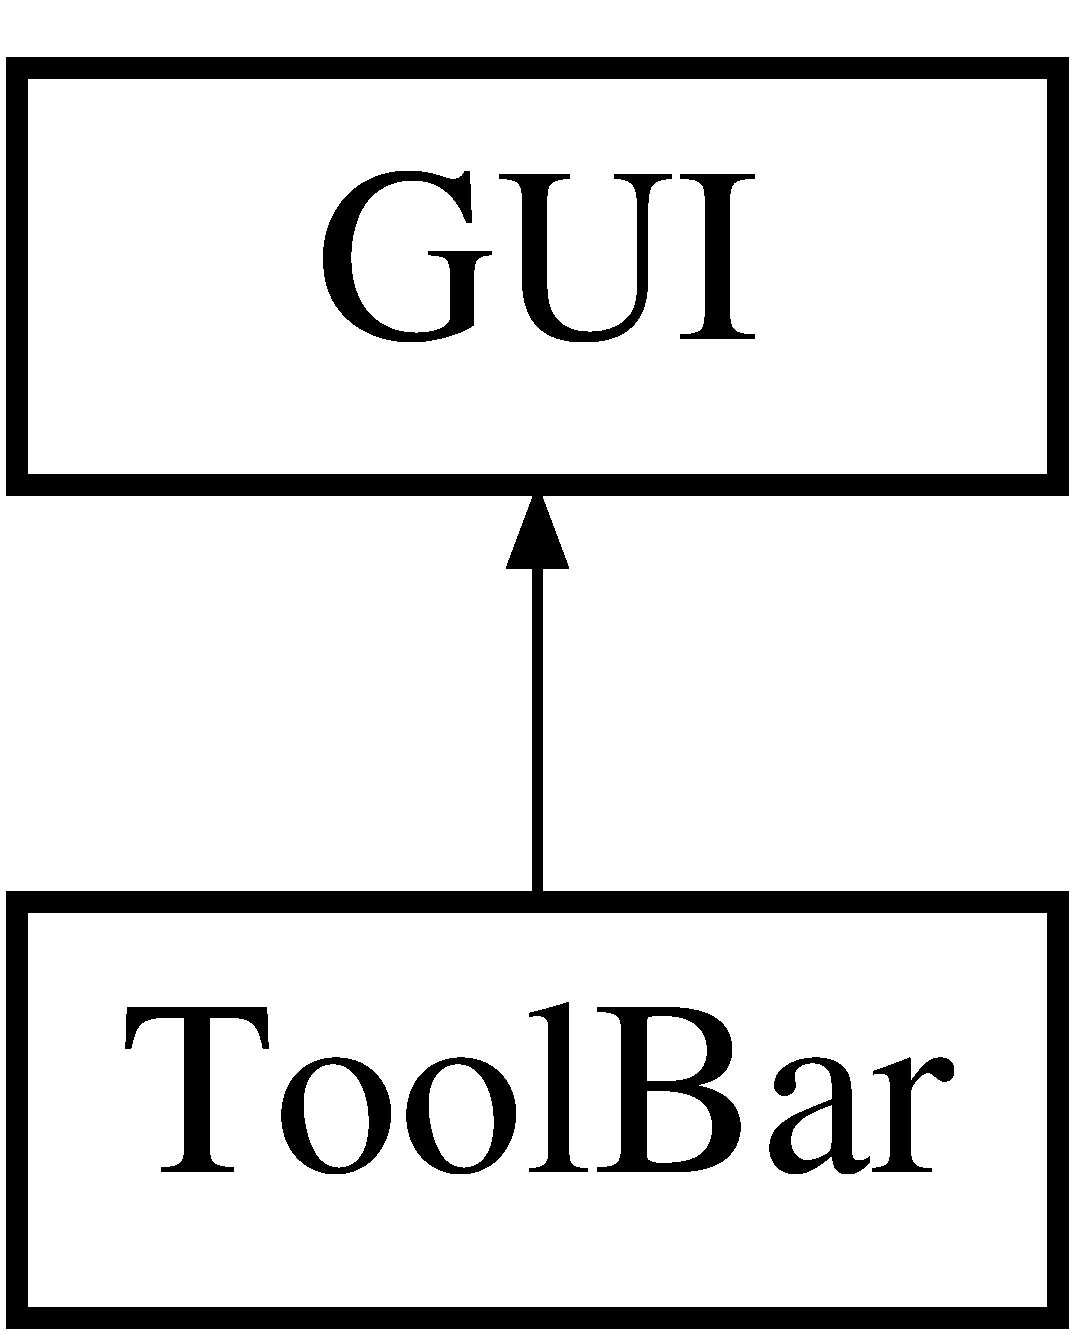
\includegraphics[height=2.000000cm]{class_tool_bar}
\end{center}
\end{figure}
\subsection*{Public Member Functions}
\begin{DoxyCompactItemize}
\item 
\mbox{\Hypertarget{class_tool_bar_a224d1f79e59de7c3e4e322f6f078abc0}\label{class_tool_bar_a224d1f79e59de7c3e4e322f6f078abc0}} 
void \hyperlink{class_tool_bar_a224d1f79e59de7c3e4e322f6f078abc0}{Render\+Toolbar} (S\+D\+L\+\_\+\+Renderer $\ast$renderer, int \&W\+I\+N\+D\+O\+W\+\_\+\+W\+I\+D\+TH, int \&W\+I\+N\+D\+O\+W\+\_\+\+H\+E\+I\+G\+HT, int \&mouseX, int \&mouseY)
\begin{DoxyCompactList}\small\item\em Function that renders the toolbar. \end{DoxyCompactList}\item 
\mbox{\Hypertarget{class_tool_bar_a1a8a8f07ea9d3173804636a13f71ea2a}\label{class_tool_bar_a1a8a8f07ea9d3173804636a13f71ea2a}} 
void {\bfseries Tool\+Bar\+Functionality} (\hyperlink{class_level}{Level} \&level, \hyperlink{class_room_design}{Room\+Design} \&designroom, \hyperlink{class_docking_doors}{Docking\+Doors} \&dockingdoors, \hyperlink{class_hydroponics}{Hydroponics} \&hydroponics, std\+::vector$<$ \hyperlink{class_hydroponics}{Hydroponics} $>$ \&all\+Hydroponics\+Farms, S\+D\+L\+\_\+\+Renderer $\ast$renderer, int \&mouseX, int \&mouseY)
\item 
\mbox{\Hypertarget{class_tool_bar_ae8124fd65ff427d4ebe91a3fe527b346}\label{class_tool_bar_ae8124fd65ff427d4ebe91a3fe527b346}} 
int \hyperlink{class_tool_bar_ae8124fd65ff427d4ebe91a3fe527b346}{get\+Toolbar\+Selection} () const
\begin{DoxyCompactList}\small\item\em The getters and setters for the toolbar selection. \end{DoxyCompactList}\item 
\mbox{\Hypertarget{class_tool_bar_a60072cabff543469021f6c96e01c0ae2}\label{class_tool_bar_a60072cabff543469021f6c96e01c0ae2}} 
int {\bfseries set\+Toolbar\+Selection} (int new\+Toolbar\+Selection)
\item 
\mbox{\Hypertarget{class_tool_bar_af2d73f6b3b39033f22f53e88502c0ff7}\label{class_tool_bar_af2d73f6b3b39033f22f53e88502c0ff7}} 
int \hyperlink{class_tool_bar_af2d73f6b3b39033f22f53e88502c0ff7}{get\+Toolbar\+SizeX} ()
\begin{DoxyCompactList}\small\item\em Getters. \end{DoxyCompactList}\item 
\mbox{\Hypertarget{class_tool_bar_a765fc1fd92c33e1bf4ee1655a3cbf513}\label{class_tool_bar_a765fc1fd92c33e1bf4ee1655a3cbf513}} 
int {\bfseries get\+Toolbar\+SizeY} ()
\item 
\mbox{\Hypertarget{class_tool_bar_a6aef146b5f26c3676021d337a062e4ec}\label{class_tool_bar_a6aef146b5f26c3676021d337a062e4ec}} 
int {\bfseries get\+Toolbar\+Xpos} ()
\item 
\mbox{\Hypertarget{class_tool_bar_aebd047f20c4174f899c69b5845c26de9}\label{class_tool_bar_aebd047f20c4174f899c69b5845c26de9}} 
int {\bfseries get\+Toolbar\+Ypos} ()
\item 
\mbox{\Hypertarget{class_tool_bar_a098fa7169404bbbac83de16f051b007b}\label{class_tool_bar_a098fa7169404bbbac83de16f051b007b}} 
int {\bfseries set\+Toolbar\+SizeX} (int newsizeX)
\item 
\mbox{\Hypertarget{class_tool_bar_a4d6dc59dfed61edcbf582ab517452a95}\label{class_tool_bar_a4d6dc59dfed61edcbf582ab517452a95}} 
int {\bfseries set\+Toolbar\+SizeY} (int newsizeY)
\item 
\mbox{\Hypertarget{class_tool_bar_aed8ebab9a9f370ee7136530a9a40bc96}\label{class_tool_bar_aed8ebab9a9f370ee7136530a9a40bc96}} 
int {\bfseries set\+Toolbar\+Xpos} (int new\+Xpos)
\item 
\mbox{\Hypertarget{class_tool_bar_ac49f60a752329fb27010b438e8e6cd40}\label{class_tool_bar_ac49f60a752329fb27010b438e8e6cd40}} 
int {\bfseries set\+Toolbar\+Ypos} (int new\+Ypos)
\end{DoxyCompactItemize}
\subsection*{Public Attributes}
\begin{DoxyCompactItemize}
\item 
\mbox{\Hypertarget{class_tool_bar_afb2a8ae55fe6b6f59ba33c414d2d507d}\label{class_tool_bar_afb2a8ae55fe6b6f59ba33c414d2d507d}} 
\hyperlink{class_texture}{Texture} \hyperlink{class_tool_bar_afb2a8ae55fe6b6f59ba33c414d2d507d}{tool\+Bar\+Background}
\begin{DoxyCompactList}\small\item\em Is the texture for the toolbar background. \end{DoxyCompactList}\item 
\mbox{\Hypertarget{class_tool_bar_a1941719914acb71c6d47638cb69a3ebe}\label{class_tool_bar_a1941719914acb71c6d47638cb69a3ebe}} 
\hyperlink{class_texture}{Texture} \hyperlink{class_tool_bar_a1941719914acb71c6d47638cb69a3ebe}{room\+Cell}
\begin{DoxyCompactList}\small\item\em Is the texture for the room cell. \end{DoxyCompactList}\item 
\mbox{\Hypertarget{class_tool_bar_a381c33f1861fdcddfc0f266ae1bcc22b}\label{class_tool_bar_a381c33f1861fdcddfc0f266ae1bcc22b}} 
\hyperlink{class_texture}{Texture} \hyperlink{class_tool_bar_a381c33f1861fdcddfc0f266ae1bcc22b}{empty\+Cell}
\begin{DoxyCompactList}\small\item\em Is the texture for teh empty cell. \end{DoxyCompactList}\item 
\mbox{\Hypertarget{class_tool_bar_ace6dfeb246713c08e8ea2705a3f597be}\label{class_tool_bar_ace6dfeb246713c08e8ea2705a3f597be}} 
\hyperlink{class_texture}{Texture} \hyperlink{class_tool_bar_ace6dfeb246713c08e8ea2705a3f597be}{empty\+Cell\+Icon}
\begin{DoxyCompactList}\small\item\em Is the texture for the empty cell icon. \end{DoxyCompactList}\item 
\mbox{\Hypertarget{class_tool_bar_a98b31dbb137739c3213075ab2076e718}\label{class_tool_bar_a98b31dbb137739c3213075ab2076e718}} 
\hyperlink{class_texture}{Texture} \hyperlink{class_tool_bar_a98b31dbb137739c3213075ab2076e718}{Door\+Texture}
\begin{DoxyCompactList}\small\item\em Is the texture for the door. \end{DoxyCompactList}\item 
\mbox{\Hypertarget{class_tool_bar_a60544cb328690f8e55537dc45b830b2e}\label{class_tool_bar_a60544cb328690f8e55537dc45b830b2e}} 
\hyperlink{class_texture}{Texture} \hyperlink{class_tool_bar_a60544cb328690f8e55537dc45b830b2e}{Hydroponics\+Icon\+Texture}
\begin{DoxyCompactList}\small\item\em Is the texture for the door. \end{DoxyCompactList}\item 
\mbox{\Hypertarget{class_tool_bar_a4143f05fb2705734554828ca8cf8ceab}\label{class_tool_bar_a4143f05fb2705734554828ca8cf8ceab}} 
\hyperlink{class_texture}{Texture} \hyperlink{class_tool_bar_a4143f05fb2705734554828ca8cf8ceab}{Bed\+Icon\+Texture}
\begin{DoxyCompactList}\small\item\em Is the texture for the bed. \end{DoxyCompactList}\item 
\mbox{\Hypertarget{class_tool_bar_ac92c7b8005c4c16e36b4cb7e0f230415}\label{class_tool_bar_ac92c7b8005c4c16e36b4cb7e0f230415}} 
\hyperlink{class_texture}{Texture} \hyperlink{class_tool_bar_ac92c7b8005c4c16e36b4cb7e0f230415}{Ship\+Dock\+Texture}
\begin{DoxyCompactList}\small\item\em Is the texture for the ship\+Dock. \end{DoxyCompactList}\item 
\mbox{\Hypertarget{class_tool_bar_aa5575f342de731d775cdc8f4b1c35747}\label{class_tool_bar_aa5575f342de731d775cdc8f4b1c35747}} 
\hyperlink{class_texture}{Texture} \hyperlink{class_tool_bar_aa5575f342de731d775cdc8f4b1c35747}{Toilet\+Icon\+Texture}
\begin{DoxyCompactList}\small\item\em Is the texture for the toilet. \end{DoxyCompactList}\item 
\mbox{\Hypertarget{class_tool_bar_ae480899c40038817888f7b470160aded}\label{class_tool_bar_ae480899c40038817888f7b470160aded}} 
std\+::vector$<$ std\+::shared\+\_\+ptr$<$ \hyperlink{class_icon}{Icon} $>$ $>$ {\bfseries all\+Icons}
\item 
\mbox{\Hypertarget{class_tool_bar_a14472b3c0e6e18c5c10ee8ac2ae8b5f7}\label{class_tool_bar_a14472b3c0e6e18c5c10ee8ac2ae8b5f7}} 
int \hyperlink{class_tool_bar_a14472b3c0e6e18c5c10ee8ac2ae8b5f7}{toolbar\+Icon\+Size} = 50
\begin{DoxyCompactList}\small\item\em Icon\+Size. \end{DoxyCompactList}\item 
\mbox{\Hypertarget{class_tool_bar_ae81299dbf81245c5133a92d24041eb3e}\label{class_tool_bar_ae81299dbf81245c5133a92d24041eb3e}} 
int \hyperlink{class_tool_bar_ae81299dbf81245c5133a92d24041eb3e}{number\+Of\+Icons} = 7
\begin{DoxyCompactList}\small\item\em Numer of icons on the toolbar. \end{DoxyCompactList}\item 
\mbox{\Hypertarget{class_tool_bar_a829a0d2ea9ce392d5bccf8557a98a0a2}\label{class_tool_bar_a829a0d2ea9ce392d5bccf8557a98a0a2}} 
int {\bfseries mouse\+Over\+Size\+Increase} = 10
\item 
\mbox{\Hypertarget{class_tool_bar_a299ab8439d40b05d8739e7e395846d5f}\label{class_tool_bar_a299ab8439d40b05d8739e7e395846d5f}} 
int {\bfseries number\+Of\+Item1} = 15
\item 
\mbox{\Hypertarget{class_tool_bar_ab87ff8704c010de962ff509082dd6c44}\label{class_tool_bar_ab87ff8704c010de962ff509082dd6c44}} 
int {\bfseries number\+Of\+Item2} = 15
\item 
\mbox{\Hypertarget{class_tool_bar_a22ebfa09c70085c77219d5e023501d98}\label{class_tool_bar_a22ebfa09c70085c77219d5e023501d98}} 
int {\bfseries number\+Of\+Item3} = 15
\item 
\mbox{\Hypertarget{class_tool_bar_a23e26fbaeee1e1c76d3ca987c620d7be}\label{class_tool_bar_a23e26fbaeee1e1c76d3ca987c620d7be}} 
int {\bfseries number\+Of\+Item4} = 15
\item 
\mbox{\Hypertarget{class_tool_bar_a2f1831ae41fee39b8abbec9f2682f663}\label{class_tool_bar_a2f1831ae41fee39b8abbec9f2682f663}} 
int {\bfseries number\+Of\+Item5} = 15
\item 
\mbox{\Hypertarget{class_tool_bar_ae255e24f4e0f1194f72d8981428d5879}\label{class_tool_bar_ae255e24f4e0f1194f72d8981428d5879}} 
int {\bfseries number\+Of\+Item6} = 15
\item 
\mbox{\Hypertarget{class_tool_bar_a085fa326a85cf9a016d5327f048c907c}\label{class_tool_bar_a085fa326a85cf9a016d5327f048c907c}} 
bool {\bfseries fill\+Level\+With\+Cells} = true
\end{DoxyCompactItemize}


The documentation for this class was generated from the following files\+:\begin{DoxyCompactItemize}
\item 
C\+:/\+Users/\+Alastair/\+Documents/\+Git\+Hub/comp250-\/\+A\+I-\/portfolio/\+Space\+Game/\+S\+D\+L\+\_\+project/Tool\+Bar.\+h\item 
C\+:/\+Users/\+Alastair/\+Documents/\+Git\+Hub/comp250-\/\+A\+I-\/portfolio/\+Space\+Game/\+S\+D\+L\+\_\+project/Tool\+Bar.\+cpp\end{DoxyCompactItemize}

%--- End generated contents ---

% Index
\backmatter
\newpage
\phantomsection
\clearemptydoublepage
\addcontentsline{toc}{chapter}{Index}
\printindex

\end{document}
